\documentclass[a4paper,11pt,UTF8]{ctexart}
% \usepackage{mathtools}
% \usepackage{nccmath}
\usepackage{QingDa}
\graphicspath{{figs/}} 
% \usepackage{amssymb}
% \usepackage{amsmath}
% % \usepackage{txfonts}
% % \usepackage{mathdots}
% % \usepackage[classicReIm]{kpfonts}
% \usepackage{graphicx}
\begin{document}

% 首先,我们回顾一下极限的定义:\par
% 设$A$为给定常数,如果对任给的$\varepsilon>0$,存在正数$\delta$,使得当$0<|x-x_0|<\delta$时,有$|f(x)-A|<\varepsilon$,
% 则称{\fangsong 函数$f$当$x$趋于$x_0$时以$A$为极限}.\par
% % 首先,我们回顾一下极限的定义:\par
% 设$A$为给定常数,如果对任给的$\varepsilon>0$,存在正数$\delta$,使得当$0<|x-x_0|<\delta$时,有$|f(x)-A|<\varepsilon$,
% 则称{\fangsong 函数$f$当$x$趋于$x_0$时以$A$为极限}.\par
首先,要证明的结论是:\par
任取$\varepsilon>0$,存在$\delta>0$,使得当$0<|x-x_0|<\delta$时,有
    \begin{equation}
        \left|\frac{1}{g(x)}-\frac{1}{B}\right|<\varepsilon\label{eq:conclusion}
    \end{equation}
式\eqref{eq:conclusion}可化为:
\begin{equation}
    \frac{|g(x)-B|}{|B|\,|g(x)|}<\varepsilon\label{eq:2}
\end{equation}
注意到上式左侧由以下三项组成:$\mfrac{1}{|B|}$、$|g(x)-B|$与$\mfrac1{|g(x)|}$.
现在要做的,就是在已经给定的正数$\varepsilon$下,找到合适的$\delta$,然后分别判断这三项的取值范围,最后论证这三项在给定的$\delta$下乘积能够小于$\varepsilon$.\par
第一项$\frac1{|B|}$是常数;\par
对第二项$|g(x)-B|$,与第三项$\frac1{|g(x)|}$,由
\begin{equation}
    \lim_{x \to x_0} g(x)=B\label{eq:lim}
\end{equation}
可得:对于任意$\varepsilon_0>0$,能够找到$\delta_0$,使得当$0<|x-x_0|<\delta_0$时,有$|g(x)-B|<\varepsilon_0$.\\
于是:
\begin{enumerate}[label=\circled{\arabic*}]
    \item 取$\varepsilon_0=\varepsilon$,则必定存在正数$\delta_{10}$,使得当$0<|x-x_0|<\delta_{10}$时,有
        \begin{equation}
            |g(x)-B|<\varepsilon\label{eq:lim1}
        \end{equation}
    \item 取$\varepsilon_0=\frac{|B|}{2}$,则必定存在正数$\delta_2$,使得当$0<|x-x_0|<\delta_2$时,就有
        \begin{equation}
            |g(x)-B|<\frac{|B|}{2}\label{eq:lim2}
        \end{equation}
\end{enumerate}
由\circled{2},可由绝对值不等式得到
    \begin{equation}
        \frac1{|g(x)|}<\frac{2}{|B|}\label{eq:lim2-1}
    \end{equation}
取$\delta=\min\{\delta_{10},\delta_2\}$,那么,当$0<|x-x_0|<\delta$时,就同时有$0<|x-x_0|<\delta_{10}$与$0<|x-x_0|<\delta_2$成立.\\
当$0<|x-x_0|<\delta_{10}$成立时,式\eqref{eq:lim1}成立,\\
当$0<|x-x_0|<\delta_2$成立时,式\eqref{eq:lim2}成立,那么式\eqref{eq:lim2-1}也就能够成立.\\
于是,当$0<|x-x_0|<\delta$时,\eqref{eq:lim1}、\eqref{eq:lim2-1}两式就能同时成立.
这时,就有:
        \begin{equation}
            \left|\frac{1}{g(x)}-\frac{1}{B}\right|=\frac{1}{|B|}\times|g(x)-B|\times\frac{1}{|g(x)|}
            <\frac{1}{|B|}\times \varepsilon \times \frac{2}{|B|}=\frac{2\varepsilon}{|B|^2}
        \end{equation}
这与我们最终想要证明的式\eqref{eq:conclusion}还差了那么一点,所以需要稍作调整.\\
\circled{1}中,改取$\varepsilon_0=\frac{|B|^2}{2}\varepsilon$,那么,则必定存在正数$\delta_1$,使得当$0<|x-x_0|<\delta_1$时,有
\begin{equation}
    |g(x)-B|<\frac{|B|^2}{2}\varepsilon.\label{eq:lim1-1}
\end{equation}
这时,改取$\delta=\min\{\delta_{1},\delta_2\}$,那么当$0<|x-x_0|<\delta$时,可知\eqref{eq:lim1-1}、\eqref{eq:lim2-1}两式同时成立.
于是
\begin{equation}
    \left|\frac{1}{g(x)}-\frac{1}{B}\right|=\frac{1}{|B|}\times|g(x)-B|\times\frac{1}{|g(x)|}
    <\frac{1}{|B|}\times \frac{|B|^2}{2}\varepsilon \times \frac{2}{|B|}=\varepsilon
\end{equation}
这就是我们要证明的式\eqref{eq:conclusion}.




% % 首先,我们回顾一下极限的定义:\par
% 设$A$为给定常数,如果对任给的$\varepsilon>0$,存在正数$\delta$,使得当$0<|x-x_0|<\delta$时,有$|f(x)-A|<\varepsilon$,
% 则称{\fangsong 函数$f$当$x$趋于$x_0$时以$A$为极限}.\par
这是Test3内容,与Test2没区别:\par
任取$\varepsilon>0$,存在$\delta>0$,使得当$0<|x-x_0|<\delta$时,有
    \begin{equation}
        \left|\frac{1}{g(x)}-\frac{1}{B}\right|<\varepsilon
    \end{equation}
式\eqref{eq:conclusion}可化为:
\begin{equation}
    \frac{|g(x)-B|}{|B|\,|g(x)|}<\varepsilon
\end{equation}
注意到上式左侧由以下三项组成:$\frac1{|B|}$、$|g(x)-B|$与$\frac1{|g(x)|}$.
现在要做的,就是在已经给定的正数$\varepsilon$下,找到合适的$\delta$,然后分别判断这三项的取值范围,最后论证这三项在给定的$\delta$下乘积能够小于$\varepsilon$.\par
第一项$\frac1{|B|}$是常数;\par
对第二项$|g(x)-B|$,与第三项$\frac1{|g(x)|}$,由
\begin{equation}
    \lim_{x \to x_0} g(x)=B
\end{equation}
可得:对于任意$\varepsilon_0>0$,能够找到$\delta_0$,使得当$0<|x-x_0|<\delta_0$时,有$|g(x)-B|<\varepsilon_0$.\\
于是:
\begin{enumerate}[label=\circled{\arabic*}]
    \item 取$\varepsilon_0=\varepsilon$,则必定存在正数$\delta_{10}$,使得当$0<|x-x_0|<\delta_{10}$时,有
        \begin{equation}
            |g(x)-B|<\varepsilon
        \end{equation}
    \item 取$\varepsilon_0=\frac{|B|}{2}$,则必定存在正数$\delta_2$,使得当$0<|x-x_0|<\delta_2$时,就有
        \begin{equation}
            |g(x)-B|<\frac{|B|}{2}
        \end{equation}
\end{enumerate}
由\circled{2},可由绝对值不等式得到
    \begin{equation}
        \frac1{|g(x)|}<\frac{2}{|B|}
    \end{equation}
取$\delta=\min\{\delta_{10},\delta_2\}$,那么,当$0<|x-x_0|<\delta$时,就同时有$0<|x-x_0|<\delta_{10}$与$0<|x-x_0|<\delta_2$成立.\\
当$0<|x-x_0|<\delta_{10}$成立时,式\eqref{eq:lim1}成立,\\
当$0<|x-x_0|<\delta_2$成立时,式\eqref{eq:lim2}成立,那么式\eqref{eq:lim2-1}也就能够成立.\\
于是,当$0<|x-x_0|<\delta$时,\eqref{eq:lim1}、\eqref{eq:lim2-1}两式就能同时成立.
这时,就有:
        \begin{equation}
            \left|\frac{1}{g(x)}-\frac{1}{B}\right|=\frac{1}{|B|}\times|g(x)-B|\times\frac{1}{|g(x)|}
            <\frac{1}{|B|}\times \varepsilon \times \frac{2}{|B|}=\frac{2\varepsilon}{|B|^2}
        \end{equation}
这与我们最终想要证明的式\eqref{eq:conclusion}还差了那么一点,所以需要稍作调整.\\
\circled{1}中,改取$\varepsilon_0=\frac{|B|^2}{2}\varepsilon$,那么,则必定存在正数$\delta_1$,使得当$0<|x-x_0|<\delta_1$时,有
\begin{equation}
    |g(x)-B|<\frac{|B|^2}{2}\varepsilon.
\end{equation}
这时,改取$\delta=\min\{\delta_{1},\delta_2\}$,那么当$0<|x-x_0|<\delta$时,可知\eqref{eq:lim1-1}、\eqref{eq:lim2-1}两式同时成立.
于是
\begin{equation}
    \left|\frac{1}{g(x)}-\frac{1}{B}\right|=\frac{1}{|B|}\times|g(x)-B|\times\frac{1}{|g(x)|}
    <\frac{1}{|B|}\times \frac{|B|^2}{2}\varepsilon \times \frac{2}{|B|}=\varepsilon
\end{equation}
这就是我们要证明的式\eqref{eq:conclusion}.
Test3内容结束




% 



% \textbf{练习-等式与不等式的性质}

学校:\_\_\_\_\_\_\_\_\_\_\_姓名:\_\_\_\_\_\_\_\_\_\_\_班级:\_\_\_\_\_\_\_\_\_\_\_考号:\_\_\_\_\_\_\_\_\_\_\_

\textbf{一、单选题}

\textbf{1.设,则下列不等式恒成立的是( )}

\textbf{A. B. C. D.}

\textbf{【来源】}2020届湖南省衡阳市高三下学期第二次模拟数学(理)试题

\textbf{【答案】}D

\textbf{【解析】}

【分析】

利用指数函数、对数函数的单调性,以及和中间量的比较,进行大小的比较,即可得解.

【详解】

对A,由为增函数,所以,可得,A错;

对B,由,所以,可得,故B错;

对C,由 ,所以、且,故C不确定;对D,由,可得:,故D对;

故选:D

【点睛】

本题考查了指数和对数的比较大小,考查了不等式性质和转化思想,属于中档题.

\textbf{2.等比数列的公比为,则与的大小关系是( )}

\textbf{A. B.}

\textbf{C. D.不能确定}

\textbf{【来源】}沪教版(上海)高三年级新高考辅导与训练第四章数列与数学归纳法一、等差数列与等比数列

\textbf{【答案】}A

\textbf{【解析】}

【分析】

要比较与的大小,只需要判断的正负即可.

【详解】

解:由等比数列的通项公式可得,,,

,,,即.

故选:.

【点睛】

本题考查了等比数列的通项公式的应用、利用作差法比较代数式的大小,关键是考查基本运算能力,属于中档题.

\textbf{3.若,把,2,2\emph{ab}中最大与最小者分别( )}

\textbf{A.\emph{,2ab} B.\emph{2ab,2} C.\emph{,2} D.\emph{2,2ab}}

\textbf{【来源】}陕西省宝鸡市烽火中学2018-2019学年高二上学期期中数学(文理)试题

\textbf{【答案】}D

\textbf{【解析】}

【分析】

由条件及不等式的性质即可求出.

【详解】

因为,

所以,

故,

故选:D

【点睛】

本题考查了不等式的基本性质和基本不等式的性质,属于基础题.

\textbf{4.命题:若,则,;命题:,使得,则下列命题中为真命题的是( )}

\textbf{A. B. C. D.}

\textbf{【来源】}山东省济宁市2018届高三上学期期末考试 数学(文)试题

\textbf{【答案】}C

\textbf{【解析】}

对于命题,当时不成立,故命题为假命题;

对于命题,当时成立,故命题为真命题.

故为真命题.选C.

\textbf{5.下列不等式中错误的是( )}

\textbf{A.若,则 B.若,则}

\textbf{C.若,则 D.若,则}

\textbf{【来源】}广西南宁市第三中学2017-2018学年高二下学期第一次月考数学(理)试题

\textbf{【答案】}D

\textbf{【解析】}

由不等式的对称性可知选项\emph{A}正确,

由不等式的传递性可知选项\emph{B}正确,

结合不等式的性质可知选项\emph{C}正确,

时,有,选项\emph{D}错误.

本题选择\emph{D}选项.

\textbf{6.设a\textgreater0,b\textgreater0,则以下不等式中不恒成立的是(
)}

\textbf{A.(a+b)≥4
B.a\textsuperscript{3}+b\textsuperscript{3}≥2ab\textsuperscript{2}}

\textbf{C.a\textsuperscript{2}+b\textsuperscript{2}+2≥2a+2b D.}

\textbf{【来源】}高中数学人教A版选修2-2 第二章 推理与证明 2.2.1
综合法和分析法(2)

\textbf{【答案】}B

\textbf{【解析】}

∵a\textgreater0,b\textgreater0,

∴(a+b)()=2++≥4恒成立.

又a\textsuperscript{2}+b\textsuperscript{2}+2-(2a+2b)=(a-1)\textsuperscript{2}+(b-1)\textsuperscript{2}≥0,

∴a\textsuperscript{2}+b\textsuperscript{2}+2≥2a+2b恒成立.

当a≥b时,( )\textsuperscript{2}=a-b.

而()\textsuperscript{2}=a+b-2

=a-b+2b-2

=(a-b)+2().

∵a≥b\textgreater0,∴≤0.

∴(a-b)+2()≤a-b,

即≥.

当a\textless b时, \textgreater0.而\textless0,

∴≥成立.

答案:B

\textbf{7.给出下列不等式:①;② ;③.其中恒成立的不等式的个数为( )}

\textbf{A.3 B.2 C.1 D.0}

\textbf{【来源】}2018-2019学年人教A版数学必修5第三章不等式单元综合测试题

\textbf{【答案】}C

\textbf{【解析】}

【分析】

根据不等式的性质,利用作差法逐项检验即可求出.

【详解】

因为,所以①正确;

因为,,所以②③错误.

故恒成立的不等式的个数为1.

【点睛】

本题主要考查了不等式的基本性质,作差比较法,属于中档题.

\textbf{8.已知实数、、满足且,则下列不等式一定成立的是( )}

\textbf{A. B. C. D.}

\textbf{【来源】}安徽省蚌埠市2017-2018学年高一下学期期末考试数学试题

\textbf{【答案】}D

\textbf{【解析】}

分析:先根据得到,即,再结合,利用不等式的基本性质即可得到结果.

详解:∵,∴,即,

又∵,∴,故选D.

点睛:本小题主要考查不等关系与不等式应用、不等式的基本性质、实数的性质等基础知识,考查运算求解能力,属于基础题.

\textbf{9.若则下列不等关系中,不能成立的是( )}

\textbf{A. B. C. D.}

\textbf{【来源】}上海市桃浦中学2018-2019学年高二上学期期末数学试题

\textbf{【答案】}B

\textbf{【解析】}

【分析】

根据不等式的性质,利用作差比较和幂函数的单调性,逐项判定,即可求解.

【详解】

由题意知,,则

对于A中,因为,所以,所以A是正确的;

对于B中,因为,所以,所以B不正确;

对于C中,因为幂函数在单调递减函数,所以,所以C正确;

对于D\\
中,因为,所以,所以D正确;

故选B.

【点睛】

本题主要考查了不等式的基本性质,以及幂函数的单调性的应用,其中解答中熟练应用作差比较法,以及幂函数的单调性,进行比较是解答的关键,着重考查了推理与运算能力,属于基础题.

\textbf{10.若正实数,满足,则有下列结论:①;②;③;④.其中正确结论的个数为(
)}

\textbf{A.1 B.2 C.3 D.4}

\textbf{【来源】}安徽省安庆市2018-2019学年高一下学期期末教学质量监测数学试题

\textbf{【答案】}C

\textbf{【解析】}

【分析】

根据不等式的基本性质,逐项推理判断,即可求解,得到答案.

【详解】

由题意,正实数是正数,且,

①中,可得,所以是错误的;

②中,由,可得是正确的;

③中,根据实数的性质,可得是正确的;

④中,因为,所以是正确的,

故选C.

【点睛】

本题主要考查了不等式的性质的应用,其中解答中熟记不等式的基本性质,合理推理是解答的关键,着重考查了推理与运算能力,属于基础题.

\textbf{11.已知函数的定义域是,当,时,若,,,则有的值( )}

\textbf{A.恒等于零 B.恒小于零}

\textbf{C.恒大于零 D.可能小于零,也可能大于零}

\textbf{【来源】}天津市2019年3月九校联考高三数学(理)学科试题

\textbf{【答案】}C

\textbf{【解析】}

【分析】

由题意可得函数为奇函数,利用导函数的解析式可得:在时,函数为增函数,进而可得时,函数为增函数,结合函数的奇偶性和函数的单调性确定的符号即可.

【详解】

函数的定义域关于原点对称,且满足,故函数为奇函数,

又由,在时恒成立,

故时,函数为增函数,进而可得时,函数为增函数,

若,

则,

则,,,

从而:,,,

据此可得:,

即的值恒大于零.

故选\emph{C}.

【点睛】

本题主要考查函数的单调性,函数的奇偶性,不等式的性质及其应用等知识,意在考查学生的转化能力和计算求解能力.

\textbf{12.若,下列不等式成立的是( )}

\textbf{A. B. C. D.}

\textbf{【来源】}甘肃省武威市第六中学2016-2017学年高一下学期期末考试数学试题

\textbf{【答案】}A

\textbf{【解析】}

由不等式的性质,若,则:

, , , .

本题选择A选项.

\textbf{13.设, ,若,则( )}

\textbf{A. B. C. D.}

\textbf{【来源】}北京市海淀区2017届高三下学期期中考试数学理试题

\textbf{【答案】}B

\textbf{【解析】}A项,若异号不成立,错误;B项,
为递增函数,故正确;C项,若则无意义,错误;D项,函数不单调,故无法判断大小关系;综上可知选B.

\textbf{14.若}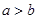
\includegraphics[width=0.38547in,height=0.19794in]{media/image151.png}\textbf{,}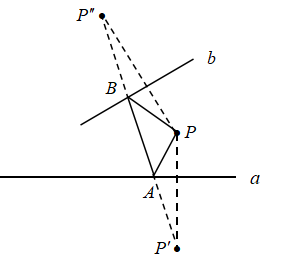
\includegraphics[width=0.40631in,height=0.19794in]{media/image152.png}\textbf{,则不等式一定成立的是(
)}

\textbf{A.}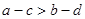
\includegraphics[width=0.88554in,height=0.19794in]{media/image153.png}
\textbf{B.}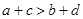
\includegraphics[width=0.8647in,height=0.19794in]{media/image154.png}
\textbf{C.}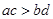
\includegraphics[width=0.55216in,height=0.19794in]{media/image155.png}
\textbf{D.}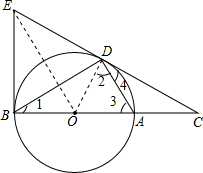
\includegraphics[width=0.53132in,height=0.21878in]{media/image156.png}

\textbf{【来源】}2015-2016学年贵州省凯里一中高二下期中数学试卷(带解析)

\textbf{【答案】}B

\textbf{【解析】}

由同向不等式的可加性可知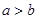
\includegraphics[width=0.38547in,height=0.19794in]{media/image157.png},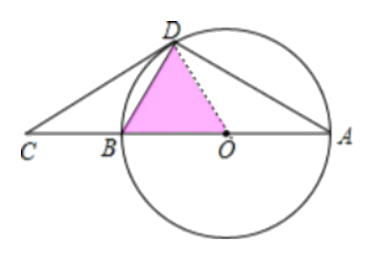
\includegraphics[width=0.40631in,height=0.19794in]{media/image158.png}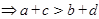
\includegraphics[width=1.03139in,height=0.19794in]{media/image159.png}成立.故选B.

考点:不等式的基本性质.

\textbf{15.如果}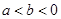
\includegraphics[width=0.63551in,height=0.19794in]{media/image160.png}\textbf{,那么下列各式一定成立的是(
)}

\textbf{A.}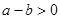
\includegraphics[width=0.62509in,height=0.19794in]{media/image161.png}
\textbf{B.}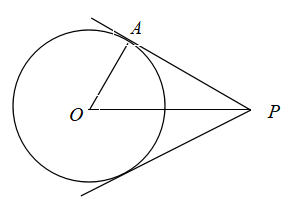
\includegraphics[width=0.54174in,height=0.19794in]{media/image162.png}
\textbf{C.}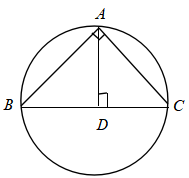
\includegraphics[width=0.51049in,height=0.21878in]{media/image163.png}
\textbf{D.}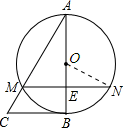
\includegraphics[width=0.44798in,height=0.42714in]{media/image164.png}

\textbf{【来源】}2015-2016学年青海平安一中高二4月月考文科数学试卷(带解析)

\textbf{【答案】}C

\textbf{【解析】}

试题分析:A中应为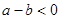
\includegraphics[width=0.63551in,height=0.19794in]{media/image165.png},B中当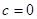
\includegraphics[width=0.38547in,height=0.19794in]{media/image166.png}时不成立,D应为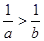
\includegraphics[width=0.4584in,height=0.42714in]{media/image167.png},故应选C.

考点:不等式的性质.

\textbf{16.已知整数a,b,c,t满足:2\textsuperscript{a}+2\textsuperscript{b}=2\textsuperscript{c},t=}\(\frac{a + b}{c}\)\textbf{,则log\textsubscript{2}t的最大值是(
)}

\textbf{A.0 B.log\textsubscript{2}3 C.2 D.3}

\textbf{【来源】}2015届四川省成都市第七中学高三一诊模拟理科数学试卷(带解析)

\textbf{【答案】}C

\textbf{【解析】}

不妨设a≤b,\(2^{b} < 2^{c} = 2^{a} + 2^{b} \leq 2^{b} + 2^{b} = 2^{b + 1} \Rightarrow b < c \leq b + 1\),

∵b,c∈Z,∴c=b+1,

\(\therefore 2^{b + 1} = 2^{a} + 2^{b}\)
\(\Rightarrow a = b = c - 1\).\(\therefore t = \frac{a + b}{c}\)
\(= 2 - \frac{2}{c}\).

∵a,t∈Z,∴c=±1,±2,∴t=0,1,3,4,故\({(\log_{2}t)}_{\max} = \log_{2}4 = 2\).

考点:指数与对数性质,不等式

\textbf{17.若a=2\textsuperscript{0.6},b=log\textsubscript{2}2,c=ln0.6,则(
)}

\textbf{A.a>b>c B.b>a>c C.c>a>b D.b>c>a}

\textbf{【来源】}2015-2016学年江西省高安中学高一重点上期中数学卷(带解析)

\textbf{【答案】}A

\textbf{【解析】}

试题分析:,故,故选A.

考点:指数与对数

\textbf{18.已知函数,若,,,则 (▲ )}

\textbf{A. B. C. D.}

\textbf{【来源】}2011届广东省华附、省实、广雅三校广州一模后联合适应性考试数学理卷

\textbf{【答案】}B

\textbf{【解析】}

本题考查函数的单调性.利用函数单调性比较数的大小.

因为,且函数是减函数,所以

即故选B

\textbf{19.设,,,则( )}

\textbf{A. B. C. D.}

\textbf{【来源】}安徽省阜阳市太和第一中学2020-2021学年高三上学期第一次校本教材反馈测试数学(文)试题

\textbf{【答案】}B

\textbf{【解析】}

【分析】

根据指数函数的单调性判断,再由作商法判断.

【详解】

因为函数是减函数,所以,所以

,所以,

所以

故选:B

【点睛】

本题主要考查了利用指数函数的单调性比较大小,属于中档题.

\textbf{20.下列不等式一定成立的是( )}

\textbf{A. B.}

\textbf{C. D.}

\textbf{【来源】}宁夏六盘山高级中学2019-2020学年高二上学期期中数学(理)试题

\textbf{【答案】}C

\textbf{【解析】}

【分析】

利用不等式的性质及基本不等式依次判断各选项即可得出.

【详解】

解:对于:,,故不成立;

对于:当时,当且仅当时取等号;

当时,当且仅当时取等号;故错误;

对于:,,故正确.

对于:等价于,即,故得,而题设,当时不成立.故错误;

故选:

【点睛】

本题考查了基本不等式的性质,考查了灵活解决问题的能力,属于基础题.

\textbf{21.已知,,则的取值范围是(  )}

\textbf{A. B. C. D.}

\textbf{【来源】}广东省潮州市2019届高三第二次模拟考试数学(理)试题

\textbf{【答案】}C

\textbf{【解析】}

【分析】

利用待定系数法求得,由,,结合,从而可得结果.

【详解】

令

则,

∴,

又,\ldots∴①

,

∴\ldots②

∴①②得.

则.

故选C.

【点睛】

本题主要考查不等式的性质以及指数函数的性质,意在考查综合运用所学知识解答问题的能力,属于中档题.

\textbf{22.已知等比数列满足,则的取值范围是( )}

\textbf{A. B. C. D.}

\textbf{【来源】}第十九篇求参数范围02---2020年高考数学选填题专项测试(文理通用)

\textbf{【答案】}D

\textbf{【解析】}

【分析】

设公比为\emph{q},根据等比数列的通项公式可得,①,,②,,③,再根据不等式的性质可得结果.

【详解】

设公比为\emph{q},∵\emph{a}\textsubscript{1}∈(0,1),\emph{a}\textsubscript{2}∈(1,2),\emph{a}\textsubscript{3}∈(3,4),

所以,①

,②

,③

所以,④

③×④得,⑤

由①得⑥,由③得⑦,

,得或⑧,

由⑤⑧可得:,

因为\emph{a}\textsubscript{4}=\emph{a}\textsubscript{3}\emph{q},∴..

故选:D

【点睛】

本题考查了等比数列的通项公式,考查了不等式的性质,属于中档题.

\textbf{23.若\emph{a}、\emph{b}、,且,则下列不等式中一定成立的是( )}

\textbf{A. B. C. D.}

\textbf{【来源】}江西省新余市第四中学2017-2018学年高二上学期期末数学(理)试题

\textbf{【答案】}D

\textbf{【解析】}

【分析】

利用不等式的性质证明,或者构造反例说明,即得解.

【详解】

由题意可知,\emph{a}、\emph{b}、,且

\emph{A}.若,满足,则,故本选项不正确;

\emph{B}.若,满足,则,故本选项不正确;

\emph{C}. 若,则,故本选项不成立;

\emph{D}.

故选:\emph{D}

【点睛】

本题考查了利用不等式的性质,判断代数式的大小,考查了学生综合分析,转化与划归的能力,属于基础题.

\textbf{24.下列不等式:①﹔②;③;④,其中恒成立的是( )}

\textbf{A.①④ B.③④ C.②③ D.①②}

\textbf{【来源】}沪教版(上海)高一第一学期新高考辅导与训练第2章不等式2.8基本不等式及其应用(1)

\textbf{【答案】}C

\textbf{【解析】}

【分析】

结合不等式的性质逐个验证.

【详解】

①当时,,不成立;

②因为,所以成立;

③易知,若,则,;

若,则,.

所以成立;

④,当或\emph{a},\emph{b}中仅有一个为0时成立,当时不成立.

故选:C

【点睛】

本题考查不等式的性质,属于基础题.

\textbf{25.设,给出下列三个结论:①;②;③.其中所有的正确结论的序号是 (
)}

\textbf{A.①③ B.①② C.②③ D.①②③}

\textbf{【来源】}福建省福州八县一中2018-2019学年高二上学期期中考试数学(理)试题

\textbf{【答案】}B

\textbf{【解析】}

【分析】

由题意逐一分析所给的说法是否正确即可.

【详解】

逐一分析所给的不等式:

由于,故,结合可得,说法①正确;

由于,故幂函数在区间上单调递减,结合可得,说法②正确;

由于,故,

对数函数单调递减,故,说法③错误.

综上可得:所有的正确结论的序号是①②.

本题选择\emph{B}选项.

【点睛】

本题主要考查不等式的性质,对数函数的单调性,幂函数的单调性等知识,意在考查学生的转化能力和计算求解能力.

\textbf{26.已知a=log\textsubscript{2}3.6,b=log\textsubscript{4}3.2,c=log\textsubscript{4}3.6,则(
).}

\textbf{A.a\textgreater b\textgreater c
B.a\textgreater c\textgreater b}

\textbf{C.b\textgreater a\textgreater c
D.c\textgreater a\textgreater b}

\textbf{【来源】}2013届浙江省温州市龙湾中学高三上学期期初考试文科数学试卷(带解析)

\textbf{【答案】}B

\textbf{【解析】}

试题分析:利用换底公式可得a=log\textsubscript{2}3.6=log\textsubscript{4}3.6\textsuperscript{2},然后根据对数函数y=log\textsubscript{4}x在(0,+∞)的单调性可进行比较即可.

解:∵a=log\textsubscript{2}3.6=log\textsubscript{4}3.6\textsuperscript{2}

∵y=log\textsubscript{4}x在(0,+∞)单调递增,

又∵3.6\textsuperscript{2}>3.6>3.2∴log\textsubscript{4}3.6\textsuperscript{2}>log\textsubscript{4}3.6>log\textsubscript{4}3.2

即a>c>b

故选B

点评:本题考查利用对数函数的单调性比较对数值大小,考查了换底公式的应用,是基础题.

\textbf{27. 设则下列判断中正确的是( )}

\textbf{A. B.}

\textbf{C. D.}

\textbf{【来源】}2016届黑龙江省大庆实验中学高三12月月考理科数学试卷(带解析)

\textbf{【答案】}B

\textbf{【解析】}

试题分析:令,则,故选B.

考点:特殊值法.

\textbf{28.已知函数,若,,则}

\textbf{A. B.}

\textbf{C. D.与的大小不能确定}

\textbf{【来源】}2011届浙江省杭州学军中学高三第一次月考理科数学卷

\textbf{【答案】}A

\textbf{【解析】}

【分析】

【详解】

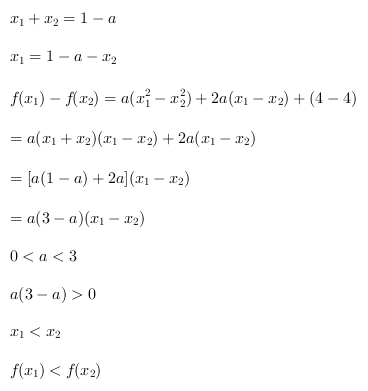
\includegraphics[width=3.83333in,height=4.07292in]{media/image305.png}

故选A.

\textbf{29.甲、乙两人连续两天在同一个水果店购买了同一品种的砂糖橘,两天的价格不同,两人购买的方式不同,每人每天购买1次,甲每次总是买5斤,乙每次总是买20元的,设甲两次购买的平均价格为\emph{x}元斤,乙两次购买的平均价格为\emph{y}元斤,则下列关系式一定成立的是(
)}

\textbf{A. B.}

\textbf{C. D.}

\textbf{【来源】}陕西省西安中学2020-2021学年高三上学期第二次月考数学(文)试题

\textbf{【答案】}D

\textbf{【解析】}

【分析】

由题意求出得到的大小关系,然后由不等式的性质,对数函数,正弦函数的性质判断.

【详解】

设砂糖橘第一天的价格是元/斤,第二天价格是元/斤,,,

则,,

∵,∴,即,

∴,,A错;;B错;

在上不是单调函数,C错;

,∴,D正确.

故选:D.

【点睛】

本题考查不等式的性质,考查对数函数,正弦函数的性质,掌握作差法比较两实数的大小是解题基础.

\textbf{30.实数,,满足,,若,则( )}

\textbf{A. B. C. D.}

\textbf{【来源】}2.2综合拔高练

\textbf{【答案】}B

\textbf{【解析】}

【分析】

由题分析,三个数中必然一个为正,两个为负,可设,则,,先对进行通分,得,通过判断分子的正负即可求解

【详解】

因为且,所以不妨设,则,,

则.

因为,,所以,又,

所以,又,所以.

故选:B.

【点睛】

本题考查分式的正负判断,通过合理变形和代换是解题关键,属于中档题

\textbf{31.若,则下列不等式不成立的是( )}

\textbf{A. B.}

\textbf{C. D.}

\textbf{【来源】}2.1不等式的基本性质(2)

\textbf{【答案】}B

\textbf{【解析】}

【分析】

利用不等式的基本性质,对选项逐一分析,选出正确选项

【详解】

由,

选项A:利用数轴可得,则,根据不等式的性质,,则,故A成立;

选项B:由于,根据``如果,那么''可得,故B不成立;

选项C:由于,两边同乘,可得,对,对其左右两边同乘,得,即,故,即,故C成立;

选项D:,,故,故D成立;综上,选B

【点睛】

本题考查不等关系与不等式,考查熟练运用不等式的基本性质灵活证明命题的能力。

\textbf{32.设,.下列说法正确的是( )}

\textbf{A.则 B.则}

\textbf{C.则 D.则}

\textbf{【来源】}杭州新东方高一数学试卷224

\textbf{【答案】}B

\textbf{【解析】}

【分析】

举反例说明C,D不成立,再根据函数单调性,进而确定选项.

【详解】

因为所以CD不成立;

因为在上单调递增,所以由得,

故选:B

【点睛】

本题考查利用函数单调性判断命题真假,考查基本分析判断能力,属基础题.

\textbf{33.设 则下列关系正确的是}

\textbf{A. B. C. D.}

\textbf{【来源】}湖北省沙市中学2018-2019学年高一12月月考数学试题

\textbf{【答案】}C

\textbf{【解析】}

【分析】

由幂函数,指数函数,对数函数的单调性以及不等式的性质判断即可.

【详解】

A.,由幂函数 当函数在上单调递减,可知A错误;

由,由不等式的性质可得,故B错误;由指数函数
当函数在上单调递减,可知C正确;由对函数 当函数在上单调递减,可知D错误.

故选 C .

【点睛】

本题考查幂函数,指数函数,对数函数的单调性以及不等式的性质,属基础题.

\textbf{34.已知,则下列不等式一定成立的是}

\textbf{A. B. C. D.}

\textbf{【来源】}天津市和平区2019届高三下学期第一次质量调查数学(文)试题

\textbf{【答案】}D

\textbf{【解析】}

【分析】

由可得,故,据此逐一考查所给的选项是否正确即可.

【详解】

由可得,故,逐一考查所给的选项:

\emph{A}.;

\emph{B}.,的符号不能确定;

\emph{C}.;

\emph{D}..

本题选择\emph{D}选项.

【点睛】

本题主要考查对数函数的性质,不等式的性质及其应用等知识,意在考查学生的转化能力和计算求解能力.

\textbf{35.对于任意实数\emph{a},\emph{b},\emph{c},\emph{d},有下列命题:}

\textbf{①若\emph{a}\textgreater{}\emph{b},\emph{c}≠0,则\emph{ac}\textgreater{}\emph{bc};②若\emph{ac}\textsuperscript{2}\textgreater{}\emph{bc}\textsuperscript{2},则\emph{a}\textgreater{}\emph{b};}

\textbf{③若\emph{a}\textgreater{}\emph{b},则;④若\emph{a}\textgreater{}\emph{b}\textgreater0,\emph{c}\textgreater{}\emph{d},则\emph{ac}\textgreater{}\emph{bd}.}

\textbf{其中真命题的个数是( )}

\textbf{A.1 B.2 C.3 D.4}

\textbf{【来源】}2.1 命题、定理、定义 学案-苏教版高中数学必修第一册

\textbf{【答案】}A

\textbf{【解析】}

【分析】

根据不等式的性质作出判断即可.

【详解】

当\emph{c}\textless0时,①错误;\emph{ac}\textsuperscript{2}\textgreater{}\emph{bc}\textsuperscript{2},显然\emph{c}\textsuperscript{2}\textgreater0,因此②正确;当\emph{a}\textgreater0\textgreater{}\emph{b}时,③错误;当\emph{a}=2,\emph{b}=1,\emph{c}=-1,\emph{d}=-2时,显然④错误

故选:A

【点睛】

本题主要考查了判断命题的真假,涉及了不等式性质的应用,属于中档题.

\textbf{36.下列结论正确的是( )}

\textbf{A.若,则 B.若,则}

\textbf{C.若,则 D.若,则}

\textbf{【来源】}湖北省武汉市外国语学校2019-2020学年高一下学期5月月考数学试题

\textbf{【答案】}C

\textbf{【解析】}

【分析】

取特殊值判断ABD,根据不等式的性质判断C.

【详解】

对于A,取时,,则A错误;

对于B,取时,,则B错误;

对于C,因为,所以由不等式的性质可知,则C正确;

对于D,取时,,则D错误;

故选:C

【点睛】

本题主要考查了根据所给条件判断不等式是否成立,属于中档题.

\textbf{37.设,且,,,则与的大小关系为( ).}

\textbf{A. B. C. D.不确定}

\textbf{【来源】}沪教版(上海)高三年级新高考辅导与训练第二章不等式二、不等式证明

\textbf{【答案】}B

\textbf{【解析】}

【分析】

,讨论和两种情况,根据对数函数单调性得到答案.

【详解】

,

当时,,函数单调递增,故;

当时,,函数单调递减,故;

综上所述:.

故选:B.

【点睛】

本题考查了比较对数式的大小,意在考查学生的计算能力和分类讨论能力,利用函数单调性是解题的关键.

\textbf{38.下列命题正确的是}

\textbf{A.若 a>b,则a\textsuperscript{2}>b\textsuperscript{2}
B.若a>b,则 ac>bc}

\textbf{C.若a>b,则a\textsuperscript{3}>b\textsuperscript{3}
D.若a\textgreater b,则 <}

\textbf{【来源】}领军考试2018届高三阶段性测评(四)晋豫省际大联考(12月)
数学(理)

\textbf{【答案】}C

\textbf{【解析】}

对于,若,,则不成立;对于,若,则不成立;对于,若,则,则正确;对于,,,则不成立.

故选C

\textbf{39.,,下列命题正确的是( )}

\textbf{A.若,则 B.若,则}

\textbf{C.若,则 D.若,则}

\textbf{【来源】}山东省潍坊市第七中学2017-2018学年高二上学期期中考试数学试题

\textbf{【答案】}B

\textbf{【解析】}

当,则,则,故错误;当时,必有,则可得,故正确;令,则,满足,但,故错误;令,则,但,故错误,故选B.

\textbf{40.若}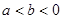
\includegraphics[width=0.65634in,height=0.19794in]{media/image417.png}\textbf{.则下列不等式中成立的是(
)}

\textbf{A.}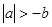
\includegraphics[width=0.54174in,height=0.28129in]{media/image418.png}
\textbf{B.}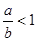
\includegraphics[width=0.38547in,height=0.42714in]{media/image419.png}
\textbf{C.}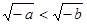
\includegraphics[width=0.90638in,height=0.25003in]{media/image420.png}
\textbf{D.}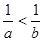
\includegraphics[width=0.44798in,height=0.42714in]{media/image421.png}

\textbf{【来源】}广西桂林中学2017-2018学年高二上学期期中考试数学(文)试题

\textbf{【答案】}A

\textbf{【解析】}

,,所以B,D错误,

∵ ,∴ C错误,故选A.

\textbf{41.设x,y,z是互不相等的正数,则下列不等式中不恒成立的是( )}

\textbf{A.}

\textbf{B.}

\textbf{C.}

\textbf{D.}

\textbf{【来源】}2016届湖北襄阳五中高三5月二模文科数学试卷(带解析)

\textbf{【答案】}C

\textbf{【解析】}

【分析】

【详解】

试题分析:,故D恒成立;

由于函数,在单调递减;在单调递增, 当时,

即,当,即正确,即A正确;

由于,故B恒成立,

若,不等式不成立, 故C不恒成立,故选C.

考点:1、基本不等式证明不等式;2、单调性证明不等式及放缩法证明不等式.

\textbf{42.设,则的大小顺序是 ( )}

\textbf{A. B. C. D.}

\textbf{【来源】}松原市乾安县第七中学2016-2017学年高二下学期期末考试数学(文)试题

\textbf{【答案】}C

\textbf{【解析】}

三个数不能直接比较大小的,又因为三个数均为正数,所以平方之后再比较大小

所以,,所以,所以,选C.

\textbf{43.若,,则( )}

\textbf{A. B. C. D.}

\textbf{【来源】}2017届河北省石家庄市第二中学高三下学期模拟联考数学(文)试卷(带解析)

\textbf{【答案】}B

\textbf{【解析】}

由题意得,因为,则,

所以,故选B.

考点:实数指数幂的运算.

\textbf{44.若不等式}\(a > b\)\textbf{与}\(\frac{1}{a} > \frac{1}{b}\)\textbf{同时成立,则必有(
)}

\textbf{A.}\(a > b > 0\) \textbf{B.}\(0 > \frac{1}{a} > \frac{1}{b}\)
\textbf{C.}\(a > 0 > b\) \textbf{D.}\(\frac{1}{a} > \frac{1}{b} > 0\)

\textbf{【来源】}2013-2014学年河南省郑州一中高二上学期期中考试理科数学试卷(带解析)

\textbf{【答案】}C

\textbf{【解析】}

试题分析:因为两个不等式同时成立,利用2个等价关系可以得到a与b的关系.\(\because\frac{1}{a} > \frac{1}{b} \Rightarrow \frac{1}{a} - \frac{1}{b} > 0 \Rightarrow \frac{b - a}{\text{ab}} > 0\)又因为\(a > b\)所以\(ab < 0\).故答案为C

考点:不等式的性质

\textbf{45.对于非空集合A、B,定义运算:}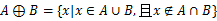
\includegraphics[width=2.26073in,height=0.21878in]{media/image460.png}\textbf{.已知}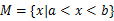
\includegraphics[width=1.18767in,height=0.21878in]{media/image461.png}\textbf{,}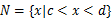
\includegraphics[width=1.16683in,height=0.21878in]{media/image462.png}\textbf{,其中a、b、c、d满足}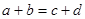
\includegraphics[width=0.88554in,height=0.19794in]{media/image463.png}\textbf{,}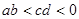
\includegraphics[width=0.82303in,height=0.19794in]{media/image464.png}\textbf{,则}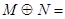
\includegraphics[width=0.67718in,height=0.19794in]{media/image465.png}\textbf{(
)}

\textbf{A.}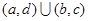
\includegraphics[width=0.91679in,height=0.21878in]{media/image466.png}
\textbf{B.}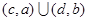
\includegraphics[width=0.91679in,height=0.21878in]{media/image467.png}

\textbf{C.}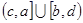
\includegraphics[width=0.8647in,height=0.23962in]{media/image468.png}
\textbf{D.}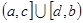
\includegraphics[width=0.8647in,height=0.23962in]{media/image469.png}

\textbf{【来源】}2015届广东省肇庆市高三第三次统一检测理科数学试卷(带解析)

\textbf{【答案】}D

\textbf{【解析】}

试题分析:本题可先由知M=\{x\textbar a<x<b\},N=\{x\textbar c<x<d\},其中a、b、c、d满足a+b=c+d,ab<cd<0,得到a,b,0,c,d的大小关系,再由新定义M⊕N的意义即可求出.

由已知M=\{x\textbar a<x<b\},∴a<b,又ab<0,∴a<0<b,同理可得c<0<d,

\(\because ab<cd<0,c<0,b>0,\therefore\frac{a}{c}>\frac{d}{b},\therefore\frac{a - c}{c}>\frac{d - b}{b},\)

\(\because a + b = c + d,\therefore a - c = d - b,\therefore\frac{d - b}{c}>\frac{d - b}{b},\)又∵c<0,b>0,∴d-b<0,因此,a-c<0,

∴a<c<0<d<b,∴M∩N=N,∴M⊕N=\{x\textbar a<x≤c,或d≤x<b\}=(a,c{]}∪{[}d,b).故选D.

考点:新定义、函数的性质,集合的运算、不等式的性质

\textbf{46.已知三角形的三边长分别为,设,则}

\textbf{与的大小关系是( )}

\textbf{A. B. C. D.}

\textbf{【来源】}20102011学年湖北省黄冈中学高二下学期期中考试文科数学卷

\textbf{【答案】}D

\textbf{【解析】}

【分析】

利用放缩法比较,利用作差法比较,从而可得结果.

【详解】

因为

所以,故选D.

【点睛】

本题主要考查``作差法''比较两个数的大小,属于简单题.
比较两个数的大小主要有四种方法:(1)作差法;(2)作商法;(3)函数单调性法;(4)基本不等式法.

\textbf{47.给出下列四个命题:}

\textbf{①若集合A,B满足,则;}

\textbf{②给定命题,若``\,''为真,则``\,''为真;}

\textbf{③设若,则;}

\textbf{④若直线与直线垂直,则.}

\textbf{其中正确命题的个数是}

\textbf{A.1 B.2 C.3 D.4}

\textbf{【来源】}烟台市中英文学校2010届高三一模考试文科数学试题

\textbf{【答案】}B

\textbf{【解析】}

【分析】

【详解】

因为,则,所以①正确;

若``\,''为真,则``\,''不一定为真,所以②错误;

若,则,所以③错误;

若直线与直线垂直,则,所以④正确

选B.

\textbf{48.下列命题正确的是( )}

\textbf{A.若,则 B.若,则}

\textbf{C.若,则 D.若,则}

\textbf{【来源】}宁夏回族自治区银川市宁夏育才中学2019-2020学年高二上学期期中数学(理)试题

\textbf{【答案】}D

\textbf{【解析】}

【分析】

\emph{A}项中,需要看分母的正负;\emph{B}项和\emph{C}项中,已知两个数平方的大小只能比较出两个数绝对值的大小.

【详解】

\emph{A}项中,若,则有,故\emph{A}项错误;\emph{B}项中,若,则,故\emph{B}项错误;\emph{C}项中,若则即,故\emph{C}项错误;\emph{D}项中,若,则一定有,故\emph{D}项正确.

故选:\emph{D}

【点睛】

本题主要考查不等关系与不等式,属于基础题.

\textbf{49.已知,给出下列命题:}

\textbf{①若,则; ②若,则;}

\textbf{③若,则; ④若,则.}

\textbf{其中真命题的个数是( )}

\textbf{A.1 B.2 C.3 D.4}

\textbf{【来源】}浙江省十校联盟2019-2020学年高三下学期寒假返校考试数学试题

\textbf{【答案】}B

\textbf{【解析】}

【分析】

①若,则,然后两边平方,再通过作差法即可得解;

②若,则,然后利用立方差公式可知,再结合以及不等式的性质即可判断;

③若,则,再利用,得出,从而求得的范围,进而判断;

④取特殊值,,即可判断.

【详解】

解:①若,

则,

所以,

所以,即①错误;

若,

则,

即,

因为,

所以,

所以,

所以,即,所以②正确;

若,

则,

因为,所以,

所以,即③正确;

④取,,满足,

但,所以④错误;

所以真命题有②③,

故选:B.

【点睛】

本题考查命题真假的判断,涉及根据不等式的性质证明不等式、指对运算法则、立方差公式等,考查学生的分析能力和运算能力.

\textbf{50.已知定义在上的函数,正实数满足,则( )}

\textbf{A. B. C. D.}

\textbf{【来源】}2020届陕西省安康市高三教学质量检测第四次联考数学(文)试题

\textbf{【答案】}C

\textbf{【解析】}

【分析】

求导可判断函数在上单调递增,即可得到,结合不等式的性质,可得到,进而可得出的大小关系.

【详解】

因为,所以函数在上单调递增,所以,

则,即,

又,所以.

由,可得;由可得,

所以.

故选:C.

【点睛】

本题考查函数单调性的应用,考查不等式的性质,考查学生的推理论证能力,属于中档题.

\textbf{51.是等比数列,是等差数列,,公差,公比,则与的大小关系为(
).}

\textbf{A. B. C. D.不确定}

\textbf{【来源】}沪教版(上海)高三年级新高考辅导与训练第四章数列与数学归纳法本章测试

\textbf{【答案】}C

\textbf{【解析】}

【分析】

先根据等差数列与等比数列通项公式求,再根据条件得,最后根据作差法,结合二项式定理放缩确定大小.

【详解】

所以

故选:C

【点睛】

本题考查等差数列与等比数列通项公式、作差法,二项式定理,考查综合分析论证能力,属中档题.

\textbf{52.已知点在直线上,且满足,则的取值范围为( )}

\textbf{A. B.}

\textbf{C. D.}

\textbf{【来源】}山东省泰安肥城市2020届高三适应性训练(一)数学试题

\textbf{【答案】}B

\textbf{【解析】}

【分析】

由,求出的取值范围,再求的范围.

【详解】

由题意,,

∵,∴,解得,

,

∵,∴或,

∴或,所以.

故选:B.

【点睛】

本题考查直线方程,考查不等式的性质,解题过程是利用点在直线上,且满足的不等关系求出的范围,然后再利用不等式的性质求解.

\textbf{53.若实数\emph{a}>\emph{b},则下列结论成立的是(   )}

\textbf{A.\emph{a}\textsuperscript{2}>\emph{b}\textsuperscript{2} B.
C.\emph{ln}2\emph{\textsuperscript{a}}>\emph{ln}2\emph{\textsuperscript{b}}
D.\emph{ax}\textsuperscript{2}>\emph{bx}\textsuperscript{2}}

\textbf{【来源】}四川省成都市温江区2018-2019学年高一下学期期末数学试题

\textbf{【答案】}C

\textbf{【解析】}

【分析】

特值法排除A,B,D,单调性判断C

【详解】

由题意,可知:

对于\emph{A}:当\emph{a}、\emph{b}都是负数时,很明显\emph{a}\textsuperscript{2}<\emph{b}\textsuperscript{2},故选项\emph{A}不正确;

对于\emph{B}:当\emph{a}为正数,\emph{b}为负数时,则有,故选项\emph{B}不正确;

对于\emph{C}:∵\emph{a}>\emph{b},∴2\emph{\textsuperscript{a}}>2\emph{\textsuperscript{b}}>0,∴\emph{ln}2\emph{\textsuperscript{a}}>\emph{ln}2\emph{\textsuperscript{b}},故选项\emph{C}正确;

对于\emph{D}:当\emph{x}=0时,结果不成立,故选项\emph{D}不正确;

故选:\emph{C}.

【点评】

本题主要考查不等式的性质应用,特殊值技巧的应用,指数函数、对数函数值大小的比较.本题属中档题.

\textbf{54.下列命题中,正确的是( )}

\textbf{A.若,,则 B.若,则}

\textbf{C.若,则 D.若,,则}

\textbf{【来源】}宁夏石嘴山市第一高级中学2019-2020学年高二上学期期末数学试题

\textbf{【答案】}C

\textbf{【解析】}

【分析】

利用不等式的基本性质进行逐项判断即可,不成立的举反例.

【详解】

对于选项A:若,满足,,但是不成立,故选项A错误;

对于选项B:若,满足,但不成立,故选项B错误;

对于选项C:因为,整理化简可得,因为,所以,即成立,故选项C正确;

对于选项D:若,满足,,但是不成立,故选项D错误;

【点睛】

本题考查不等式与不等关系;不等式的基本性质的灵活运用是求解本题的关键;属于中档题、常考题型.

\textbf{55.若,则下列不等式中不成立的是( )}

\textbf{A. B. C. D.\emph{a}\textsuperscript{5} +
\emph{b}\textsuperscript{5} \textless{}
\emph{a}\textsuperscript{2}\emph{b}\textsuperscript{3} +
\emph{a}\textsuperscript{3}\emph{b}\textsuperscript{2}}

\textbf{【来源】}福建省莆田市第一中学2018-2019学年高二上学期第一次月考数学(文)试题

\textbf{【答案】}B

\textbf{【解析】}

【分析】

根据不等式的性质判断A,C,根据作差法判断C,举反例判断B.

【详解】

由于a<b<0,则\textbar a\textbar>\textbar b\textbar,即,故A正确,

当a=-2,b=-1时, ,故B不正确,\\
由a<b<0,两边同时除以ab可得,故C正确,\\
,\\
故D正确.

故选B.

【点睛】

本题考查不等式的性质,解题的关键是利用不等式的性质,不正确结论,列举反例.

\textbf{56.已知,以下一定成立的是( )}

\textbf{A. B. C. D.}

\textbf{【来源】}浙江省宁波效实中学2018-2019学年高一上学期期中考试数学试题

\textbf{【答案】}D

\textbf{【解析】}

【分析】

根据不等式性质推导D,举反例说明A,B ,C不成立.

【详解】

2\textgreater1\textgreater0\textgreater-1\textgreater-2,21=-1(-2),2(-1)=1(-2),,A,B,C错;

因为,所以,因此,即得,D对.

【点睛】

本题考查不等式性质,考查基本分析判断能力.

\textbf{57.已知:,则3,,的大小关系是( )}

\textbf{A. B.}

\textbf{C. D.}

\textbf{【来源】}湖南省益阳市2019届高三4月模拟考试数学(理)试题

\textbf{【答案】}D

\textbf{【解析】}

【分析】

先将指数式化为对数式,再根据对数函数单调性以及运算法则比较大小,确定选项.

【详解】

,,

∴;

又 ,∴.故选D.

【点睛】

本题考查指数式化与对数式关系以及对数函数单调性,考查基本分析求解能力,属基础题.

\textbf{58.设,,,且,则( )}

\textbf{A. B. C. D.}

\textbf{【来源】}福建省漳州市2016-2017学年高一下学期期末考试数学试题

\textbf{【答案】}C

\textbf{【解析】}

若,则不成立,故答案A错误;若,则不成立,故答案B错误;因为,所以,则由不等式的性质对不等式两边同乘以可得
,即,故答案C 正确;若,则答案D不正确,应选答案C.

\textbf{59.已知,且,下列不等式中,一定成立的是 ( )}

\textbf{①;②;③;④}

\textbf{A.①② B.③④ C.②③ D.①④}

\textbf{【来源】}广东省中山一中2018届高三级第五次统测试卷理科数学试题

\textbf{【答案】}B

\textbf{【解析】}

,且当时,,

故① 错误; ,且,即,,故② 错误;,且 ,,故③ 正确;,且, ,故④
正确,故选B.

\textbf{60.已知且,则的取值范围是( )}

\textbf{A. B. C. D.}

\textbf{【来源】}浙江省台州市五校2019-2020学年高一下学期期中联考数学试题

\textbf{【答案】}B

\textbf{【解析】}

【分析】

由已知条件推导出,,再由得出,由得出,结合不等式的基本性质可求得的取值范围.

【详解】

,,则,,,则,

由得,则,即,即,

又,,因此,的取值范围是.

故选:B.

【点睛】

本题考查代数式取值范围的求解,考查不等式基本性质的应用,考查计算能力,属于中等题.

\textbf{61.设,且,则( )}

\textbf{A. B. C. D.}

\textbf{【来源】}安徽省亳州市第二中学2018-2019学年高二上学期期中数学(文)试题

\textbf{【答案】}C

\textbf{【解析】}

【分析】

取特殊值判断\emph{A,D},根据不等式的性质判断\emph{B},根据幂函数的性质判断\emph{C}.

【详解】

\emph{A}选项,取时,不等式不成立;

\emph{B}选项,不等式两边加上同一个数,不等号方向不发生改变,故错误;

\emph{C}选项,根据幂函数在R上为增函数知,故正确;

\emph{D}选项,取,不等式不成立,故错误.

故选:\emph{C}

【点睛】

本题主要考查了不等式的性质,幂函数的单调性,特值法,属于中档题.

\textbf{62.若\emph{a}>\emph{b},\emph{c}为实数,下列不等式成立是()}

\textbf{A.\emph{ac}>\emph{bc} B.\emph{ac}<\emph{bc} C. D.}

\textbf{【来源】}陕西省黄陵中学本部2018-2019学年高二下学期期末考试数学(文)试题

\textbf{【答案】}D

\textbf{【解析】}

【分析】

由已知条件,利用不等式的基本性质,直接求解,即可得到答案.

【详解】

由题意,为实数,

在A中,当时,不定成立,所以不正确;

在B中,当时,不定成立,所以不正确;

在C中,当时,不定成立,所以不正确;

在D中,因为,所以成立,故选D.

【点睛】

本题主要考查了不等式的基本性质的应用,其中解答中熟记不等式的基本性质,合理推理、运算是解答的关键,着重考查了推理与运算能力,属于基础题.

\textbf{63.对于实数\emph{a},\emph{b},\emph{c},给出下列命题:①若\emph{a}>\emph{b},则\emph{ac}\textsuperscript{2}>\emph{bc}\textsuperscript{2};②若0>\emph{a}>\emph{b},则;③若\emph{a}>\emph{b},,则\emph{a}>0,\emph{b}<0;④若\emph{a}>\emph{b}>\emph{c}>0,则.其中真命题的个数为(  )}

\textbf{A.0 B.1 C.2 D.3}

\textbf{【来源】}上海市建平中学2015-2016学年高一上学期期中数学试题

\textbf{【答案】}C

\textbf{【解析】}

【分析】

举例说明①错误;利用基本不等式的性质推得②正确;举例说明③错误;利用分析法说明④正确.

【详解】

①若\emph{a}>\emph{b},则\emph{ac}\textsuperscript{2}>\emph{bc}\textsuperscript{2},错误,当\emph{c}\textsuperscript{2}=0时,\emph{ac}\textsuperscript{2}=\emph{bc}\textsuperscript{2};

②若0>\emph{a}>\emph{b},则,把\emph{a}>\emph{b}两边同时乘以,得,即正确;

③当\emph{a}>\emph{b}>0或\emph{b}<\emph{a}<0时,有,③错误;

④\emph{a}>\emph{b}>\emph{c}>0,则\emph{a}+\emph{c}>0,\emph{b}+\emph{c}>0,若成立,则\emph{ab}+\emph{ac}>\emph{ab}+\emph{bc},即

\emph{ac}>\emph{bc},也就是\emph{a}>\emph{b},此时成立,故④正确.

所以真命题的个数是2.

故选:C

【点睛】

本题考查命题的真假判断与应用,考查了基本不等式的性质,属于基础题.

\textbf{64.已知实数,则下列不等关系中错误的是( )}

\textbf{A. B.}

\textbf{C. D.}

\textbf{【来源】}2020届重庆市巴蜀中学高考适应性月考卷(四)数学(理)试题

\textbf{【答案】}D

\textbf{【解析】}

【分析】

对每个不等式进行判断.也可举反例说明不成立.

【详解】

∵,

∴,A正确;

,B正确;

,C正确;

若,满足,但,D错误.

故选:D.

【点睛】

本题考查不等式的证明,不等式的证明可用作差法比较大小,也可用综合法进行证明,还可用反证法证明,如果不等式不成立可以举反例说明.

\textbf{65.若,,则  }

\textbf{A. B. C. D.}

\textbf{【来源】}四川省眉山一中办学共同体2019届高三10月月考数学(理)试卷

\textbf{【答案】}D

\textbf{【解析】}

【分析】

运用不等式对四个选项逐一分析

【详解】

对于,,,,则,故错误

对于,若,则,即,这与矛盾,故错误

对于,,,,则,故错误

对于,,,故正确

故选

【点睛】

本题考查了不等式的性质,由未知数的范围确定结果,属于基础题.

\begin{quote}
\textbf{66.设函数,若对任意恒成立,则实数x的取值范围是  }
\end{quote}

\textbf{A. B. C. D.}

\textbf{【来源】}山东省烟台市2018-2019学年高一上学期期中考试数学试题

\textbf{【答案】}B

\textbf{【解析】}

【分析】

将不等式左边构造为以为自变量的函数,其图象是直线,其最值在区间两端点处取得.

【详解】

因为,可化为:对任意恒成立,

令,则,即,解得:,

故选.

【点睛】

本题考查了不等式恒成立问,求解过程中运用了更换主元的方法,转化为直线问题,代入端点求出结果,属中档题.

\textbf{67.设,若,,则与的大小关系是( )}

\textbf{A. B. C. D.不能确定}

\textbf{【来源】}吉林省舒兰市第一高级中学校2018-2019学年高二下学期第一次月考数学(文)试题

\textbf{【答案】}B

\textbf{【解析】}

【分析】

对S和T进行分子有理化,然后通过作差比较即可得到结论.

【详解】

,

,

又,

所以S-T\textless0,即S\textless T

故选B

【点睛】

本题考查利用作差法比较大小关系,属于基础题.

\textbf{68.设,且,则( )}

\textbf{A. B. C. D.}

\textbf{【来源】}2014-2015学年福建省德化一中高二上学期第一次质检文科数学试卷(带解析)

【答案】D

\textbf{【解析】}

试题分析:A.,时不成立,B.,时不成立,C.

也不成立,D.只要,恒成立

考点:不等式成立问题.

\textbf{69.设,则的大小关系是}

\textbf{A. B. C. D.}

\textbf{【来源】}2014-2015学年山东省枣庄市四十二中高一上学期期中考试数学试卷(带解析)

\textbf{【答案】}B

【解析】

试题分析:因为,故

考点:指数函数、对数函数的图像和性质.

\textbf{70.若,则与的大小关系为( )}

\textbf{A. B. C. D.不能确定}

\textbf{【来源】}海南省海南中学1011学年高二下学期期末考试数学(文)

\textbf{【答案】}B

\textbf{【解析】}本题考查不等式性质;比较两个数的大小的方法:比较法

因为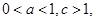
\includegraphics[width=1.00014in,height=0.21878in]{media/image728.png}所以

则所以故选B

\textbf{71.对于实数,``\,''是``\,''的( )}

\textbf{A.充分不必要条件 B.必要不充分条件}

\textbf{C.充要条件 D.既不充分也不必要条件}

\textbf{【来源】}四川省成都市龙泉第二中学2018届高三10月月考数学(文)试题

\textbf{【答案】}B

\textbf{【解析】}

由``\,''可得,即``\,''成立,若``\,'',
时``\,''不成立,所以``\,''是``\,''的必要不充分条件,故选B.

【方法点睛】本题通过主要考查不等式的性质以及充分条件与必要条件,属于中档题.判断充要条件应注意:首先弄清条件和结论分别是什么,然后直接依据定义、定理、性质尝试.对于带有否定性的命题或比较难判断的命题,除借助集合思想化抽象为直观外,还可利用原命题和逆否命题、逆命题和否命题的等价性,转化为判断它的等价命题;对于范围问题也可以转化为包含关系来处理.

\textbf{72.若,,则下列不等式不正确的是( )}

\textbf{A. B. C. D.}

\textbf{【来源】}山东省东营市河口区一中2017-2018学年度第二学期普通高中模块检查高二数学(文)试题

\textbf{【答案】}D

\textbf{【解析】}

分析:根据不等式性质推导,确定选项.

详解:因为,,所以

因为,,所以

因为,,所以

因为,,所以

选D.

点睛:本题考查不等式性质,考查基本推理论证能力.

\textbf{73.已知,为正实数,}

\textbf{①若,则;}

\textbf{②若,则;}

\textbf{③若,则;}

\textbf{④若,则;}

\textbf{上述命题中正确的是( )}

\textbf{A.①② B.②③ C.③④ D.①④}

\textbf{【来源】}河南省郑州市第一中学网校2017-2018学年高二上学期期中联考数学(理)试题

\textbf{【答案】}D

\textbf{【解析】}

若,不妨取,此时;说法②错误,排除\emph{AB}选项,

若,不妨取,此时;说法③错误,排除\emph{C}选项,

本题选择\emph{D}选项.

\textbf{74.下列说法正确的是(  )}

\textbf{A.``}\(x < 1\)\textbf{''是``}\(\log_{2}\left( x + 1 \right) < 1\)\textbf{''的充分不必要条件}

\textbf{B.命题``}\(\forall x > 0\)\textbf{,}\(2^{x} > 1\)\textbf{''的否定是``}\(\exists x_{0} \leq 0\)\textbf{,}\(2^{x_{0}} \leq 1\)\textbf{''}

\textbf{C.命题``若}\(a \leq b\)\textbf{,则}\(ac^{2} \leq bc^{2}\)\textbf{''的逆命题为真命题}

\textbf{D.命题``若}\(a + b \neq 5\)\textbf{,则}\(a \neq 2\)\textbf{或}\(b \neq 3\)\textbf{''为真命题}

\textbf{【来源】}2017届云南省云南师范大学附属中学高三高考适应性月考(五)文数试卷(带解析)

\textbf{【答案】}D

\textbf{【解析】}

选项A:\(\log_{2}(x + 1) < 1 \Leftrightarrow 0 < x + 1 < 2 \Leftrightarrow - 1 < x < 1\),所以``\(x < 1\)''是其必要不充分条件;选项B:命题``\(\forall x > 0,\text{  }2^{x} > 1\)''的否定是``\(\exists x_{0} > 0,\text{  }2^{x_{0}} \leq 1\)'';选项C:命题``若\(a \leq b\),则\(ac^{2} \leq bc^{2}\)''的逆命题是``若\(ac^{2} \leq bc^{2}\),则\(a \leq b\)'',当\emph{c}=0时,不成立;选项D:其逆否命题为``若\(a = 2\)且\(b = 3\),则\(a + b = 5\)''为真命题,故原命题为真,故选D.

\textbf{75.已知,则的取值范围是 (   )}

\textbf{A. B. C. D.}

\textbf{【来源】}黑龙江省双鸭山市第一中学2017-2018学年高二4月月考数学(文)试题

\textbf{【答案】}C

\textbf{【解析】}

设

易得:,

∴

故选:C

点睛:根据不等式组确定二元目标式范围的方程有二,其一:利用待定系数法表示目标,直接加减一次即可;其二:利用线性规划的方法处理.

\textbf{76.实数,,满足且,则下列关系式成立的是( )}

\textbf{A. B. C. D.}

\textbf{【来源】}贵阳第一中学2018届高考适应性月考卷(七)理数

\textbf{【答案】}A

\textbf{【解析】}

∵∴由∴∴综上,可得 .

故选A.

\textbf{77.设集合则``\,''是``\,''的( )}

\textbf{A.充要条件 B.必要不充分条件}

\textbf{C.充分不必要条件 D.既不充分也不必要条件}

\textbf{【来源】}甘肃省兰州市第一中学2016-2017学年高二下学期期末考试数学(文)试题

\textbf{【答案】}C

\textbf{【解析】}

试题分析:,,∵,选C.

考点:1、分式不等式和绝对值不等式的解法;2、充分条件和必要条件.

\textbf{78.
已知\emph{a}=,\emph{b}=,\emph{c}=,则实数a,b,c的大小关系是(  )}

\textbf{A.a\textgreater c\textgreater b
B.b\textgreater a\textgreater c}

\textbf{C.a\textgreater b\textgreater c
D.c\textgreater b\textgreater a}

\textbf{【来源】}人教A版高中数学 高三二轮(文)专题04
基本初等函数、函数与方程 测试

\textbf{【答案】}C

\textbf{【解析】}

依题意得,

∴,

∴,

又,

∴.选\emph{C}.

\textbf{79.给出下列命题:
①若}\(a,b \in R_{+},a \neq b\)\textbf{,则}\(a^{3} + b^{3} > a^{2}b + ab^{2}\)\textbf{;
②若}\(a,b,m \in R_{+},a < b\)\textbf{,则}
\(\frac{a + m}{b + m} < \frac{a}{b}\)\textbf{;
③若}\(\frac{a}{c^{2}} > \frac{b}{c^{2}}\)\textbf{,则}\(a > b\)\textbf{;
④当}\(x \in \left( 0,\frac{\pi}{2} \right)\)\textbf{时,}\(\sin x + \frac{2}{\sin x}\)\textbf{的最小值为}\(2\sqrt{2}\)\textbf{,其中结论正确的个数为(
)}

\textbf{A.}\(1\) \textbf{B.}\(2\) \textbf{C.}\(3\) \textbf{D.}\(4\)

\textbf{【来源】}山东省济南第一中学2019-2020学年高二10月阶段性检测数学试题

\textbf{【答案】}B

\textbf{【解析】}

【分析】

对于①②利用作差法可证明不等式是否成立,对于③由不等式性质可判断,对于④由基本不等式求得最值,并判断等号能否取到即可.

【详解】

对于①,若\(a,b \in R_{+},a \neq b\),则\(\left( a^{3} + b^{3} \right) - \left( a^{2}b + ab^{2} \right) = \left( a - b \right)^{2}\left( a + b \right) > 0\)成立,即\(a^{3} + b^{3} > a^{2}b + ab^{2}\)成立,所以①正确;

对于②,若\(a,b,m \in R_{+},a < b\),则\(\frac{a + m}{b + m} - \frac{a}{b} = \frac{m\left( a - b \right)}{b\left( b + m \right)} > 0\),即\(\frac{a + m}{b + m} < \frac{a}{b}\)不成立,所以②错误;

对于③,若\(\frac{a}{c^{2}} > \frac{b}{c^{2}}\),由不等式性质两边同时乘以\(c^{2}\),可得\(a > b\),所以③正确;

对于④,当\(x \in \left( 0,\frac{\pi}{2} \right)\)时,\(\sin x + \frac{2}{\sin x} \geq 2\sqrt{2}\),当且仅当\(\sin x = \frac{2}{\sin x}\)时取等号,因为\(\sin x = \sqrt{2}\)不成立,所以④错误;

综上可知,正确的为①③;

故选:B.

【点睛】

本题考查了作差法证明不等式是否成立,不等式性质应用,基本不等式求最值及等号成立条件,属于中档题.

\textbf{80.设,则下列不等式中一定成立的是( )}

\textbf{A. B. C. D.}

\textbf{【来源】}河南省信阳市息县第一高级中学2019-2020学年高二上学期第三次阶段性考试数学(文)试题

\textbf{【答案】}C

\textbf{【解析】}

【分析】

根据不等式的性质以及特殊值法进行判断即可.

【详解】

由,得出,故A错误;

当时,,,故BD错误;

由基本不等式得,即,故C正确;

故选:C

【点睛】

本题主要考查了由已知条件判断所给不等式是否成立,属于中档题.

\textbf{81.已知,满足,则的取值范围是( )}

\textbf{A. B. C. D.}

\textbf{【来源】}安徽省六安市第一中学2017-2018学年高一下学期期末考试数学(理)试题

\textbf{【答案】}A

\textbf{【解析】}

分析:该问题是已知不等关系求范围的问题,可以用待定系数法来解决.

详解:设α+3β=λ(α+β)+v(α+2β)

=(λ+v)α+(λ+2v)β.

比较α、β的系数,得,

从而解出λ=﹣1,v=2.

分别由①、②得﹣1≤﹣α﹣β≤1,2≤2α+4β≤6,

两式相加,得1≤α+3β≤7.

故α+3β的取值范围是{[}1,7{]}.

故选A

点睛:本题考查待定系数法,考查不等式的基本性质,属于基础题.

\textbf{82.两个正实数,满足,,成等差数列,则不等式恒成立时实数的取值范围是(
)}

\textbf{A. B. C. D.}

\textbf{【来源】}福建省龙岩市一级达标校2019-2020学年高一下学期期末质检数学试题

\textbf{【答案】}C

\textbf{【解析】}

【分析】

由题意利用等差数列的定义和性质求得,再利用基本不等式求得,根据题意,,由此求得的范围.

【详解】

解:两个正实数,满足,,成等差数列,

,,,.

不等式恒成立,即恒成立,

即恒成立.

,求得,

故选:C.

【点睛】

本题主要考查等差数列的定义和性质,不等式的恒成立问题,基本不等式的应用,属于基础题.

\textbf{83.设,则下列结论中正确的是( )}

\textbf{A. B. C. D.}

\textbf{【来源】}河南省豫北重点中学2017-2018学年高二12月联考数学(理)试卷

\textbf{【答案】}D

\textbf{【解析】}

【分析】

【详解】

,A错误

当时;B错误;

当时 ;C错误;

成立;所以选D.

\textbf{84.若a>0,b>0,且a+b=4,则下列不等式中恒成立的是( )}

\textbf{A.}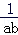
\includegraphics[width=0.18758in,height=0.36473in]{media/image843.png}\textbf{>}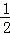
\includegraphics[width=0.10421in,height=0.36473in]{media/image844.png}
\textbf{B.}
\includegraphics[width=0.10421in,height=0.36473in]{media/image845.png}\textbf{+}
\includegraphics[width=0.10421in,height=0.36473in]{media/image846.png}\textbf{≤1
C.}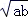
\includegraphics[width=0.29178in,height=0.18758in]{media/image847.png}\textbf{≥2
D.}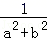
\includegraphics[width=0.48978in,height=0.42726in]{media/image848.png}\textbf{≤}
\includegraphics[width=0.10421in,height=0.36473in]{media/image849.png}

\textbf{【来源】}{[}同步{]}2014年新人教B版选修4-5
1.2基本不等式练习卷(带解析)

\textbf{【答案】}D

\textbf{【解析】}

试题分析:由题设知ab≤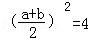
\includegraphics[width=0.92746in,height=0.42726in]{media/image850.png},所以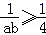
\includegraphics[width=0.47936in,height=0.36473in]{media/image851.png},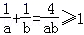
\includegraphics[width=0.87535in,height=0.36473in]{media/image852.png},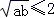
\includegraphics[width=0.56273in,height=0.18758in]{media/image853.png},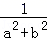
\includegraphics[width=0.48978in,height=0.42726in]{media/image854.png}=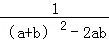
\includegraphics[width=1.13588in,height=0.4481in]{media/image855.png}=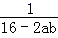
\includegraphics[width=0.60441in,height=0.39599in]{media/image856.png}≤
\includegraphics[width=0.10421in,height=0.36473in]{media/image857.png},由此能够排除选项A、B、C,从而得到正确选项.

解:∵a>0,b>0,且a+b=4,

∴ab≤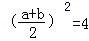
\includegraphics[width=0.92746in,height=0.42726in]{media/image858.png},

∴\includegraphics[width=0.47936in,height=0.36473in]{media/image859.png},故A不成立;

\includegraphics[width=0.87535in,height=0.36473in]{media/image860.png},故B不成立;

\includegraphics[width=0.56273in,height=0.18758in]{media/image861.png},故C不成立;

∵ab≤4,a+b=4,∴16﹣2ab≥8,

∴\includegraphics[width=0.48978in,height=0.42726in]{media/image862.png}=\includegraphics[width=1.13588in,height=0.4481in]{media/image863.png}=\includegraphics[width=0.60441in,height=0.39599in]{media/image864.png}≤\includegraphics[width=0.10421in,height=0.36473in]{media/image865.png},故D成立.

故选D.

考点:基本不等式.

\textbf{85.小茗同学的妈妈是吉林省援鄂医疗队的队员,为了迎接凯旋归来的英雄母亲,小茗准备为妈妈献上一束鲜花.据市场调查,已知6枝玫瑰花与3枝康乃馨的价格之和大于24元,而4枝玫瑰花与5枝康乃馨的价格之和小于22元,则2枝玫瑰花的价格和3枝康乃馨的价格比较结果是(
)}

\textbf{A.3枝康乃馨价格高 B.2枝玫瑰花价格高 C.价格相同 D.不确定}

\textbf{【来源】}吉林省长春实验中学2019-2020学年高一6月月考数学(理)试题

\textbf{【答案】}B

\textbf{【解析】}

【分析】

设1枝玫瑰和1枝康乃馨的价格分别元,由题意可得:,令,根据待定系数法求得,借助不等式性质即可证得.

【详解】

设1枝玫瑰和1枝康乃馨的价格分别元,由题意可得:,

令,

则,解得:

,

因此.

所以2枝玫瑰的价格高.

故选:B

【点睛】

本题考查不等关系与不等式性质,考查不等式比较大小的问题,属于中档题.

\textbf{86.若0\textless{}\emph{a}\textless{}\emph{b}且\emph{a}+\emph{b}=1,则四个数,\emph{b},2\emph{ab},中最大的是(
)}

\textbf{A. B.\emph{b} C.2\emph{ab} D.}

\textbf{【来源】}海南省海口市灵山中学2020届上学期高三第三次月考试题

\textbf{【答案】}B

\textbf{【解析】}

【分析】

由得,由且,把换为可得,下面只要比较与的大小,两数作差,再根据的范围,可得差的最大值小于0,所以最大.

【详解】

解:(1)且,,,

(2),,,

(3),

又,,

,

综上可知:最大.

故选:.

【点睛】

本题考查不等式比较大小,用到完全平方式,二次函数求最值,这种题目比较灵活,用到知识点多,不易掌握,训练逻辑推理,综合运用能力.

\textbf{87.已知,满足的解集为集合,则下列命题为真命题的是( )}

\textbf{A., B.,}

\textbf{C., D.,}

\textbf{【来源】}辽宁省实验中学2019-2020学年高一上学期第一次月考数学试题

\textbf{【答案】}C

\textbf{【解析】}

【分析】

利用整体思想,设,利用待定系数法解出与,

然后根据不等式的基本性质得出的取值范围并判断所给选项的正误.

【详解】

令,则,

解得,,

故,

又,故,

又,所以.

故选:C.

【点睛】

本题考查不等式的基本性质及运用,考查整体思想的运用,较简单.

\textbf{88.已知,,则的取值范围是( )}

\textbf{A. B. C. D.}

\textbf{【来源】}浙江省宁波市镇海中学2018-2019学年高一下学期期中数学试题

\textbf{【答案】}A

\textbf{【解析】}

【分析】

根据等式可确定的正负,利用可求得所求范围.

【详解】

,,,,

,,;

又,;

综上所述:.

故选:.

【点睛】

本题考查利用不等式的性质求范围的问题,关键是能够利用等式确定的正负.

\textbf{89.下列三个不等式中( )}

\textbf{①;②;③}

\textbf{恒成立的个数为( )}

\textbf{A. B. C. D.}

\textbf{【来源】}辽宁省重点高中协作校2019-2020学年高一上学期期末数学试题

\textbf{【答案】}B

\textbf{【解析】}

【分析】

利用作差法可判断①,利用基本不等式可判断②,根据不等式的性质及作差法可判断③.

【详解】

解:对于①,由,,,可知,可知恒成立,故①正确;

\begin{quote}
对于②,当时,,当且仅当即时取等号,

当时,,当且仅当即时取等号,故②错误;

对于③,
\end{quote}

根据正数不等式的同向可乘性得

\begin{quote}
,故③正确

故正确的有①③

故选:

【点睛】

本题主要考查了基本不等式的成立条件的判断及不等式的性质等知识的简单应用,属于基础试题
\end{quote}

\textbf{90.若,则下列不等式中成立的是( )}

\textbf{A. B. C. D.}

\textbf{【来源】}浙江省宁波市北仑中学2019-2020学年高一(2-10班)下学期期中数学试题

\textbf{【答案】}D

\textbf{【解析】}

【分析】

根据条件,利用不等式的性质.不等式两边同时乘以一个负数,不等号的方向要改变.验证即可.

【详解】

对于, ,不成立

对于.不妨取,显然不成立.

对于, ,结合,可知成立.

故选:D.

【点睛】

本题考查利用不等式的性质比较不等式大小.

利用不等式性质比较大小,要注意不等式性质成立的前提条件.解决此类问题除根据不等式的性质求解外,还经常采用特殊值验证的方法.

\textbf{91.设,,则下列不等式中不一定成立的是( )}

\textbf{A. B.}

\textbf{C. D.}

\textbf{【来源】}河北省衡水市第十三中学2019届高三质检(四)文科数学试题

\textbf{【答案】}D

\textbf{【解析】}

【分析】

举反例否定D,而A,B,C可结合函数与不等式性质给予证明.

【详解】

因为在上是增函数,所以;

因为-c在上是减函数,所以;

因为,所以

当时,,所以D不成立,选D.

【点睛】

本题考查指数函数单调性、反比例函数单调性以及不等式性质,考查基本应用求解能力.属基本题.

\textbf{92.在下列命题中,所有真命题的序号是( )}

\textbf{①若,则; ②若,则;}

\textbf{③若,则; ④若,则}

\textbf{A.① ② B.① ③ C.② ④ D.② ③ ④}

\textbf{【来源】}吉林省舒兰市第一高级中学校2018-2019学年高二下学期第一次月考数学(文)试题

\textbf{【答案】}D

\textbf{【解析】}

【分析】

利用不等式的性质对各个选项进行检验即可得到答案.

【详解】

①若,当a=0时,,故错误;

②幂函数当a=2n+1时函数在定义域上单调递增,若,则,故正确;

③若x\textgreater y,则-x\textless-y,0\textless c-x\textless c-y,
,又,由不等式的性质可知正确;

④,,故正确;

真命题的序号是② ③ ④

故选D

【点睛】

本题考查不等式性质的应用,考查分析能力,属于基础题.

\textbf{93.已知,,下列不等式成立的是( )}

\textbf{A. B.}

\textbf{C. D.}

\textbf{【来源】}安徽省合肥市一中、合肥六中2018-2019学年高一下学期期末联考数学试题

\textbf{【答案】}A

\textbf{【解析】}

【分析】

由作差法可判断出A、B选项中不等式的正误;由对数换底公式以及对数函数的单调性可判断出C选项中不等式的正误;利用指数函数的单调性可判断出D选项中不等式的正误.

【详解】

对于A选项中的不等式,,,,

,,,,A选项正确;

对于B选项中的不等式,,,,

,,,B选项错误;

对于C选项中的不等式,,,,

,,,即,C选项错误;

对于D选项中的不等式,,函数是递减函数,

又,所以,D选项错误.故选A.

【点睛】

本题考查不等式正误的判断,常见的比较大小的方法有:(1)比较法;(2)中间值法;(3)函数单调性法;(4)不等式的性质.在比较大小时,可以结合不等式的结构选择合适的方法来比较,考查推理能力,属于中等题.

\textbf{94.若a、b、c∈R,则下列命题中正确的是( )}

\textbf{A.若ac\textgreater bc,则a\textgreater b
B.若a\textgreater b,则a\textgreater b}

\textbf{C.若,则a\textgreater b D.若,则a\textgreater b}

\textbf{【来源】}二轮复习测试专项 专题四 数列与不等式

\textbf{【答案】}D

\textbf{【解析】}

若ac\textgreater bc,则c\textgreater0时
a\textgreater b;若\textgreater,则\textbar a\textbar\textgreater\textbar b\textbar;若,则a\textgreater b或a\textless0\textless b;
若,则a\textgreater b,所以选D.

\textbf{95.若a\textless b,d\textless c,并且(c-a)(c-b)\textless0,(d-a)(d-b)\textgreater0,则a,b,c,d的大小关系为(  )}

\textbf{A.d\textless a\textless c\textless b
B.a\textless d\textless c\textless b}

\textbf{C.a\textless d\textless b\textless c
D.d\textless c\textless a\textless b}

\textbf{【来源】}2019届高考数学(理)全程训练:天天练25 不等式的性质及一元二次不等式

\textbf{【答案】}A

\textbf{【解析】}因为\emph{a}\textless{}\emph{b},(\emph{c}-\emph{a})(\emph{c}-\emph{b})\textless0,所以\emph{a}\textless{}\emph{c}\textless{}\emph{b},因为(\emph{d}-\emph{a})(\emph{d}-\emph{b})\textgreater0,所以\emph{d}\textless{}\emph{a}\textless{}\emph{b}或\emph{a}\textless{}\emph{b}\textless{}\emph{d},又\emph{d}\textless{}\emph{c},所以\emph{d}\textless{}\emph{a}\textless{}\emph{b}.综上,\emph{d}\textless{}\emph{a}\textless{}\emph{c}\textless{}\emph{b}.选A.

\textbf{96.设,若,则(  )}

\textbf{A. B. C. D.}

\textbf{【来源】}上海市崇明区2018届高三第一次高考模拟考试数学试题

\textbf{【答案】}D

\textbf{【解析】}

,当时,不成立,根据对数函数的定义,可知真数必需大于零,故不成立,由于正弦函数具有周期性和再某个区间上为单调函数,故不能比较,故不成立,
根据指数函数的单调性可知,正确,故选D.

\textbf{97.设a\textgreater b\textgreater1,c\textless0,给出下列四个结论:}

\textbf{①;②;③;④.}

\textbf{其中正确的结论有( )}

\textbf{A.1个 B.2个 C.3个 D.4个}

\textbf{【来源】}河南省林州市林州一中分校高二下学期周练数学(文)试题

\textbf{【答案】}B

\textbf{【解析】}

【分析】

根据不等式的性质可判断①,根据幂函数的性质可判断②;指数函数的性质可判断③,根据对数函数的性质可判断④.

【详解】

因为,,所以 ,①正确;

因为,所以在上单调递减,则,②错误;

因为,所以在R上单调递增,则,③错误;因为,则,④正确.

综上所述,正确的结论有2个,故选B.

【点睛】

本题主要考查不等式的性质、幂函数的性质、指数函数的性质、对数函数的性质,属于简单题.
比较两个数的大小主要有三种方法:(1)作差法;(2)作商法;(3)函数单调性法;(4)基本不等式法.

\textbf{98.设,,则与的大小关系是( )}

\textbf{A. B. C. D.}

\textbf{【来源】}2015-2016学年河北武邑中学高二下5.8周考文科数学卷(带解析)

\textbf{【答案】}D

\textbf{【解析】}

试题分析:,故选.

考点: 三角形不等式.

【名师点睛】二维形式的三角不等式:设x\textsubscript{1},y\textsubscript{1},x\textsubscript{2},y\textsubscript{2}∈R,那么.

当且仅当时取等号.

\textbf{99.已知}\includegraphics{media/image1028.png}\textbf{,则p是q的(
)}

\textbf{A.充分条件但不是必要条件 B.必要条件但不是充分条件}

\textbf{C.充要条件 D.既不充分也不必要条件}

\textbf{【来源】}2015-2016学年山西省临汾一中高二上期末文科数学试卷(带解析)

\textbf{【答案】}A

\textbf{【解析】}

试题分析:通过解不等式求出命题p,q分别为真命题时对应的x的范围;再判断p成立是否能推出q成立反之q成立是否能推出p成立.

解:若P真即\includegraphics{media/image1029.png}即\includegraphics{media/image1030.png}即\includegraphics{media/image1031.png}

若q真即\includegraphics{media/image1032.png}即0<x<1

因为p成立则q成立但若q成立p不一定成立

所以p是q的充分不必要条件.

故选A

考点:充要条件.

\textbf{100.若对于任意的\emph{x}>0,不等式恒成立,则实数\emph{a}的取值范围是(
)}

\textbf{A.\emph{a}≥ B.\emph{a}> C.\emph{a}< D.\emph{a}≤}

\textbf{【来源】}山东省滨州市北镇中学2019-2020学年高一上学期9月月考数学试题

\textbf{【答案】}A

\textbf{【解析】}

【分析】

由于\emph{x}>0,对不等式左侧分子分母同时除以\emph{x},再求出左侧最大值即可求解.

【详解】

由题:对于任意的\emph{x}>0,不等式恒成立,

即对于任意的\emph{x}>0,不等式恒成立,

根据基本不等式:,当且仅当时,取得等号,

所以的最大值为,

所以.

故选:A

【点睛】

此题考查不等式恒成立求参数范围,通过转化成求解函数的最值问题,结合已学过的函数模型进行求解,平常学习中积累常见函数处理办法可以事半功倍.

\textbf{101.若,且,则下列不等式成立的是( )}

\textbf{A. B.}

\textbf{C. D.}

\textbf{【来源】}天津市耀华中学2020-2021学年高三上学期第一次月考数学试题

\textbf{【答案】}C

\textbf{【解析】}

【分析】

根据已知条件有,且,,,结合指对幂函数的性质比较的大小.

【详解】

由,且知:,

∴,,,

∴,而,即,

综上,有.

故选:C

【点睛】

本题考查了由不等关系比较大小,结合基本不等式、的关系比较大小,属于基础题.

\textbf{102.实数,,满足且,则下列关系式成立的是( )}

\textbf{A. B. C. D.}

\textbf{【来源】}吉林省白城市洮南市第一中学2020-2021学年高一第一次月考数学(理)试题

\textbf{【答案】}A

\textbf{【解析】}

【分析】

根据,变形为比较\emph{c},\emph{b},根据,变形为,再与\emph{b}作差比较.

【详解】

因为,

所以,

所以,

因为,

所以,

所以,

所以,

所以

故选:A

【点睛】

本题主要考查数的大小比较以及不等式的基本性质,还考查了转化求解问题的能力,属于中档题.

\textbf{103.若,,则下面不等式正确的是( ).}

\textbf{A. B.}

\textbf{C. D.}

\textbf{【来源】}沪教版(上海)高三年级新高考辅导与训练第二章不等式二、不等式证明

\textbf{【答案】}D

\textbf{【解析】}

【分析】

根据绝对值三角不等式得到D正确,取特殊值排除ABC得到答案.

【详解】

,则,故,D正确;

取,知AB错误;取,知C错误.

故选:D.

【点睛】

本题考查了绝对值三角不等式,判断不等关系,意在考查学生的推断能力.

\textbf{104.下列判断错误的是( )}

\textbf{A.若随机变量服从正态分布,则}

\textbf{B.已知直线平面,直线平面,则``\,''是``\,''的充分不必要条件}

\textbf{C.若随机变量服从二项分布: , 则}

\textbf{D.是的充分不必要条件}

\textbf{【来源】}2018届湖南省怀化市高三第二次模拟数学(理)试题

\textbf{【答案】}D

\textbf{【解析】}

【分析】

根据正态分布、空间中点线面的位置关系、充分条件与必要条件的判断、二项分布及不等式的性质等知识,依次对四个选项加以分析判断,进而可求解.

【详解】

对于选项,若随机变量服从正态分布,根据正态分布曲线的对称性,有,故选项正确,不符合题意;

对于选项,已知直线平面,直线平面,则当时一定有,充分性成立,而当时,不一定有,故必要性不成立,所以``\,''是``\,''的充分不必要条件,故选项正确,不符合题意;

对于选项,若随机变量服从二项分布: , 则,故选项正确,不符合题意;

对于选项,,仅当时有,当时,不成立,故充分性不成立;若,仅当时有,当时,不成立,故必要性不成立.

因而是的既不充分也不必要条件,故选项不正确,符合题意.

故选:D

【点睛】

本题考查正态分布、空间中点线面的位置关系、充分条件与必要条件的判断、二项分布及不等式的性质等知识,考查理解辨析能力与运算求解能力,属于基础题.

\textbf{105.设\emph{a},\emph{b}(1﹣\emph{x}\textsuperscript{2})\emph{dx},\emph{c}=2\emph{ln}2,则(
)}

\textbf{A.\emph{a}<\emph{b}<\emph{c}
B.\emph{b}<1<\emph{c}<\emph{a} C.\emph{c}<\emph{a}<\emph{b}
D.\emph{c}<\emph{b}<\emph{a}}

\textbf{【来源】}2019届湖南省衡阳市第八中学高三上学期第三次月考数学(理)试题

\textbf{【答案】}B

\textbf{【解析】}

【分析】

根据题意,分析可得,,,据此比较可得答案.

【详解】

根据题意,,

,

,

,

.

所以,

所以.

则有,

故选:.

【点睛】

本题主要考查定积分的计算,考查对数和分数指数幂的计算,意在考查学生对这些知识的理解掌握水平,属于基础题.

\textbf{106.下列不等式中:}

\textbf{①; ②;}

\textbf{③; ④.}

\textbf{其中正确的序号是( )}

\textbf{A.①②③④ B.①②③}

\textbf{C.①②④ D.③④}

\textbf{【来源】}广东省中山一中2017-2018学年第二学期高二级第一次段考题文科数学试题

\textbf{【答案】}B

\textbf{【解析】}

分析:由题意逐一考查所给的不等式是否成立即可.

详解:逐一考查所给的不等式:

,,

即:,整理可得:,说法①正确;

,

,,说法②正确;

,

,,说法③正确;

,

,,说法④错误;

综上可得:正确的序号是①②③.

本题选择\emph{B}选项.

点睛:本题主要考查不等式的性质的应用,实数大小的比较等知识,意在考查学生的转化能力和计算求解能力.

\begin{quote}
\textbf{107.设,则的大小关系是}
\end{quote}

\textbf{A. B. C. D.}

\textbf{【来源】}2018届北京市十一学校高三年级3月文科零模试卷

\textbf{【答案】}B

\textbf{【解析】}

0\textless\textless1,\textgreater1,\textless0,所以b\textgreater a\textgreater c,选B.

\textbf{108.已知那么下列命题中正确的是( )}

\textbf{A.若,则}

\textbf{B.若,则}

\textbf{C.若且,则}

\textbf{D.若且,则}

\textbf{【来源】}2.1等式性质与不等式性质

\textbf{【答案】}C

\textbf{【解析】}

【分析】

利用不等式的性质,给出反例说明题中的命题为假命题,或者利用不等式的性质证明题中的命题为真命题即可.

【详解】

\emph{A}中,当时,不成立,故\emph{A}错误;

\emph{B}中,当时,,故\emph{B}错误;

\emph{C}中,若,则,∴,故\emph{C}正确;

\emph{D}中,当时,满足且,但是不满足,故\emph{D}错误;

综上所述,只有选项\emph{C}的说法正确.

故选C.

【点睛】

本题主要考查不等式的性质及其应用,属于中等题.

\textbf{109.若,则下列不等式中成立的是( )}

\textbf{A. B. C. D.}

\textbf{【来源】}陕西省西安市蓝田县2018-2019学年高二下学期期末数学试题

\textbf{【答案】}A

\textbf{【解析】}

【分析】

对于\emph{A},用不等式的性质可以论证,对于\emph{B},\emph{C},\emph{D},列举反例,可以判断.

【详解】

∵\emph{a}<0,∴\textbar{}\emph{a}\textbar=﹣\emph{a},∵\emph{a}<\emph{b}<0,∴﹣\emph{a}>﹣\emph{b}>0,∴\textbar{}\emph{a}\textbar>﹣\emph{b},故结论\emph{A}成立;

取\emph{a}=﹣2,\emph{b}=﹣1,则

∵,∴\emph{B}不正确;

,∴,∴\emph{C}不正确;

,,∴,∴\emph{D}不正确.

故选:\emph{A}.

【点睛】

本题考查不等式的性质,解题的关键是利用不等式的性质,对于不正确结论,列举反例.

\textbf{110.已知不等式对一切正整数恒成立,则实数的取值范围为( )}

\textbf{A. B. C. D.}

\textbf{【来源】}江西省南康中学2019届高三上学期第五次月考数学(文)试题

\textbf{【答案】}B

\textbf{【解析】}

【分析】

先利用裂项求和法求得不等式左边各项的和,然后求得左边式子的取值范围,再根据恒成立问题列不等式,解不等式可求得的取值范围.

【详解】

不等式左边,是一个单调递增的数列,故当时取得最小值为.故,即,也即,解得.故选B.

【点睛】

本小题主要考查裂项求和法,考查数列的单调性以及最小值,考查不等式恒成问题的解题策略,考查对数不等式的解法,属于中档题.对于分母是两个等差数列相乘的数列求和,主要采用的方法是裂项求和法,裂项求和法要注意哪些项是合并的,剩下哪些项.

\textbf{111.已知,则下列不等式正确的是( )}

\textbf{A. B.}

\textbf{C. D.}

\textbf{【来源】}河南省周口市2018-2019学年高二上学期期末抽测考试数学(文)试题

\textbf{【答案】}C

\textbf{【解析】}

【分析】

根据不等式的性质,以及指数函数与对数函数的单调性,逐项判定,即可得到答案.

【详解】

由题意,因为,则

对于A中,则 ,所以,所以不正确;

对于B中,因为函数为单调递减函数,所以,所以不正确;

对于C中,因为函数为单调递增函数,又因为,则,

所以是正确的;

对于D中,由,所以,所以不正确,故选C.

【点睛】

本题主要考查了不等式的性质的应用,以及比较大小问题,其中解答中熟练应用作差法比较,以及熟记指数函数与对数函数的单调性是解答的关键,着重考查了推理与计算能力,属于基础题.

\textbf{112.若,则下列不等式中一定不成立的是( )}

\textbf{A. B. C. D.}

\textbf{【来源】}全国名校大联考2017-2018年度高三第三次联考数学(理)试题

\textbf{【答案】}A

\textbf{【解析】}

,,不正确;正确;正确;时, 成立,故选A.

\textbf{113.定义在区间区间上的函数满足: ,若时,,若,
则的大小关系为( )}

\textbf{A. B.}

\textbf{C. D.}

\textbf{【来源】}2015届辽宁省大连市高三上学期名校联考文科数学试卷(带解析)

\textbf{【答案】}B

\textbf{【解析】}

试题分析:取,则,所以,,设,则
,所以,所以,所以函数f(x)在(-1,1)上为减函数,由,得:,取,,则,所以
,因为 ,所以 ,所以R>P>Q.故选B.

考点:抽象函数的性质.

\textbf{114.已知函数,(),若任意,且都有,则实数\emph{a}的取值范围(
)}

\textbf{A. B. C. D.}

\textbf{【来源】}江西省上高二中2021届高三上学期第二次月考数学(理)试题

\textbf{【答案】}A

\textbf{【解析】}

【分析】

不妨设,对不等式进行化简,转化为恒成立,再将不等式变形,得到恒成立,进而根据和不等式恒成立的意义,结合不等式的基本性质即可求出的取值范围.

【详解】

不妨设,

=

=,

对任意且,

不等式恒成立,

时,,即恒成立

,<

,即的取值范围为;

故选:A.

【点睛】

本题考查了函数不等式恒成立求参数取值范围,也是常考题型,关键是转化思想和分离参数思想的运用.

\textbf{115.买4个苹果和5只桃子的金额之和小于22元,而买6个苹果和3只桃子的金额之和大于24元,那么买2个苹果和买3只桃子的金额比较,其结果是(
)}

\textbf{A.2个苹果贵 B.3只桃子 C.相同 D.不能确定}

\textbf{【来源】}上海市上海外国语大学附属中学2019-2020学年高一上学期期中数学试题

\textbf{【答案】}A

\textbf{【解析】}

【分析】

设苹果的单价为,桃子的单价为,再列出不等式进行求解即可.

【详解】

设苹果的单价为,桃子的单价为,由题可得,

故,由不等式性质可知,化简得.

又,由不等式性质可知,化简得.

故,即买2个苹果贵.

故选:A

【点睛】

本题主要考查了根据讲实际中的情景利用数学语言表达,再根据不等式的性质判断分析的方法等.属于中档题.

\textbf{116.对于函数(,且),下列说法:①当且时,函数为上单调增函数;②函数满足;③函数可能具有奇偶性;④当时,对于任意的,总有;其中正确的是(
)}

\textbf{A.①② B.②③ C.①②③④ D.③④}

\textbf{【来源】}江苏省百校联考2019-2020学年高一上学期第三次考试数学试题

\textbf{【答案】}C

\textbf{【解析】}

【分析】

由函数的单调性及奇偶性可得①③正确,由指数的运算可得②正确,由重要不等式的应用可得④正确.

【详解】

解:对于①,当且时,函数为上单调增函数,即①正确;

对于②,,,即,即②正确;

对于③,当时,,函数既是奇函数,由是偶函数,即③正确,

对于④,,

当且仅当,即时取等号,即④正确,

综上可得①②③④均正确,

故选:C.

【点睛】

本题考查了函数的单调性及奇偶性,重点考查了重要不等式的应用,属中档题.

\textbf{117.设实数,则下列不等式一定正确的是( )}

\textbf{A. B.}

\textbf{C. D.}

\textbf{【来源】}贵州省南白中学(遵义县一中)2018-2019学年高二下学期第一次联考数学(文)试题

\textbf{【答案】}D

\textbf{【解析】}

【分析】

对4个选项分别进行判断,即可得出结论.

【详解】

解:由于\emph{a}>\emph{b}>0,,\emph{A}错;

当0<\emph{c}<1时,\emph{c\textsuperscript{a}}<\emph{c\textsuperscript{b}};当\emph{c}=1时,\emph{c\textsuperscript{a}}=\emph{c\textsuperscript{b}};当\emph{c}>1时,\emph{c\textsuperscript{a}}>\emph{c\textsuperscript{b}},故\emph{c\textsuperscript{a}}>\emph{c\textsuperscript{b}}不一定正确,\emph{B}错;

\emph{a}>\emph{b}>0,\emph{c}>0,故\emph{ac}﹣\emph{bc}>0,\emph{C}错.

,\emph{D}对;

故选\emph{D}.

【点睛】

本题考查不等式的性质,考查学生分析解决问题的能力,属于中档题.

\textbf{118.设,下列命题正确的是 ( )}

\textbf{A.若,则 B.若,则}

\textbf{C.若,则 D.若,则}

\textbf{【来源】}浙江省丽水市四校2019届高一下学期5月阶段性联考数学试题

\textbf{【答案】}D

\textbf{【解析】}

【分析】

根据不等式的性质和用给a,b,c赋值的方法判断选项是否正确。

【详解】

当时,,有,A不正确;

当时,,有,B不正确;

当时,,有,C不正确;

由题得,有,故选D。

【点睛】

本题考查不等式的基本性质,和用赋值的方法来判断选项。

\textbf{119.若,且,则、、、中值最小的是( )}

\textbf{A. B.}

\textbf{C. D.}

\textbf{【来源】}2.4基本不等式及其应用(1)

\textbf{【答案】}C

\textbf{【解析】}

【分析】

由基本不等式,可求得,,再利用作差比较,可得,即可得到判断,即可求解.

【详解】

由题意,实数,且,

根据基本不等式,可得,当且仅当时,等号成立,

因为,所以等号不成立,所以

又由当且仅当时,等号成立,

因为,所以等号不成立,所以,

因为,,所以,

所以,即,

所以、、、中值最小的是,

故选C.

【点睛】

本题主要考查了基本不等式的应用,其中解答中熟记基本不等式的``一正、二定、三相等'',以及熟练应用基本不等式求解是解答的关键,着重考查了推理与运算能力,属于基础题.

\textbf{120.若存在,使对任意的恒成立,则( )}

\textbf{A.的最小值为 B.的最小值为}

\textbf{C.的最小值为 D.的最小值为}

\textbf{【来源】}2019年12月上海市松江区一模数学试题

\textbf{【答案】}B

\textbf{【解析】}

【分析】

先令,由题意,得到,推出,

三式相加得,根据绝对值不等式的性质定理,得到,再由题中存在,使结论成立,可得:只需,进而可得出结果.

【详解】

因为对任意的恒成立,令,

则只需,即,所以,

所以以上三式相加可得:,

由绝对值不等式的性质定理可得:,

因此只需

即.

故选:B

【点睛】

本题主要考查求最值的问题,熟记绝对值不等式的性质,以及不等式的性质即可,属于常考题型.

\textbf{121.(2018·南昌一模)已知a,b,c∈R,a+b+c=0,abc\textgreater0,T=,则(  )}

\textbf{A.T\textgreater0 B.T\textless0}

\textbf{C.T=0 D.T≥0}

\textbf{【来源】}2018届高三数学训练题(43):不等式的概念与性质

\textbf{【答案】}B

\textbf{【解析】}

取特殊值,\emph{a}=2,\emph{b}=\emph{c}=-1,

则,排除\emph{A},\emph{C},\emph{D},

本题选择\emph{B}选项.

\textbf{122.已知,则下列各不等式中一定成立的是( )}

\textbf{A. B. C. D.}

\textbf{【来源】}2020届北京市密云区高三第二学期第二次阶段性测试数学试题

\textbf{【答案】}D

\textbf{【解析】}

【分析】

取特殊值排除A,B选项,利用指数函数的性质判断C选项,利用指数函数的性质结合基本不等式,从而判断D选项.

【详解】

对A项,取,则,故A错误;

对B项,取,则,故B错误;

对C项,在上单调递减,,,故C错误;

对D项,在上单调递增,,

则,,当且仅当时取等号

即,故D正确;

故选:D

【点睛】

本题主要考查了根据已知条件判断所给不等式是否成立,涉及了指数函数性质的应用,属于中档题

\textbf{123.已知且,则下列不等式不一定成立的是( )}

\textbf{A. B. C. D.}

\textbf{【来源】}江苏省苏州市吴中区2019-2020学年高二上学期期中数学试题

\textbf{【答案】}A

\textbf{【解析】}

【分析】

由条件可得,,由不等式的性质可知B、C、D正确,对A,当时,不等式不成立.

【详解】

因为且,所以,,

对A,因为,而当时,不等式不成立,故A错误;

对B,因为,,所以,故B正确;

对C,因为,所以,又,所以,故C正确;

对D,因为,所以,又,,所以,故D正确,

故选:A

【点睛】

本题主要考查不等式与不等关系及不等式性质的简单应用,关键是要判断出,.

\textbf{124.记 则A,B,C的大小关系是( )}

\textbf{A. B. C. D.}

\textbf{【来源】}福建省闽侯第一中学2018届高三上学期开学考试数学(文)试题

\textbf{【答案】}B

\textbf{【解析】}

,即\emph{A}\textgreater{}\emph{C},

,即\emph{B}\textless{}\emph{C},

综合知\emph{A}\textgreater{}\emph{C}\textgreater{}\emph{B}.

本题选择\emph{B}选项.

\textbf{125.设实数满足约束条件,则的最小值为( )}

\textbf{A. B. C. D.}

\textbf{【来源】}湖北省黄冈中学2017年高三5月第三次模拟考试文科数学试题

\textbf{【答案】}C

\textbf{【解析】}

由约束条件可知, (当且仅当 时等号成立),即的最小值为,故选C.

【易错点晴】本题主要考查约束条件的应用、不等式的性质及利用基本不等式求最值,属于难题.利用基本不等式求最值时,一定要正确理解和掌握``一正,二定,三相等''的内涵:一正是,首先要判断参数是否为正;二定是,其次要看和或积是否为定值(和定积最大,积定和最小);三相等是,最后一定要验证等号能否成立(主要注意两点,一是相等时参数否在定义域内,二是多次用或时等号能否同时成立).

\textbf{126.已知,则这三个数的大小关系为( )}

\textbf{A. B. C. D.}

\textbf{【来源】}2016-2017学年浙江杭州西湖高级中学高一上学期期中数学试卷(带解析)

【答案】A

\textbf{【解析】}

试题分析:函数在上单调递减,所以,又,所以,故选A.

考点:指数式比较大小.

\textbf{127.若,则下列不等式中,正确的不等式有①②③④( )}

\textbf{A.4个 B.3个}

\textbf{C.2个 D.1个}

\textbf{【来源】}2016-2017学年广西南宁马山县高二上期中数学试卷(带解析)

\textbf{【答案】}C

\textbf{【解析】}

试题分析:取,代入验证,②③错误.故选C.实际上,,.

考点:不等式的基本性质.

【思路点晴】判断一个关于不等式的命题的真假时,先把要判断的命题与不等式性质联系起来考虑,找到与命题相近的性质,并应用性质判断命题的真假,当然判断的同时可能还要用到其他知识,比如对数函数、指数函数的性质.特殊值法是判断命题真假时常用到的一个方法,在命题真假未定时,先用特殊值试试,可以得到一些对命题的感性认识,如正好找到一组特殊值使命题不成立,则该命题为假命题.

\textbf{128.给出下列语句:}

\textbf{①若\emph{a},\emph{b}为正实数,\emph{a}≠\emph{b},则\emph{a}\textsuperscript{3}+\emph{b}\textsuperscript{3}>\emph{a}\textsuperscript{2}\emph{b}+\emph{ab}\textsuperscript{2};}

\textbf{②若\emph{a},\emph{b},\emph{m}为正实数,\emph{a}<\emph{b},则;}

\textbf{③若>,则\emph{a}>\emph{b};}

\textbf{④当\emph{x}∈}\includegraphics[width=0.53125in,height=0.39583in]{media/image1358.png}\textbf{时,sin
\emph{x}+}\includegraphics[width=0.3125in,height=0.32292in]{media/image1359.png}\textbf{的最小值为2}\includegraphics[width=0.19792in,height=0.20833in]{media/image1360.png}\textbf{,}

\textbf{其中结论正确的个数为(  )}

\textbf{A.0 B.1 C.2 D.3}

\textbf{【来源】}江西省横峰中学2017-2018学年高二上学期第一次月考数学(理)试题

\textbf{【答案】}C

\textbf{【解析】}

对于①,若\emph{a},\emph{b}∈\emph{R}+,\emph{a}≠\emph{b},

∵,

故\textgreater 正确;

对于②,若\emph{a},\emph{b},\emph{m}∈\emph{R}+,\emph{a}\textless{}\emph{b},

则−,

则故错;

对于③,若>,则\emph{a}>\emph{b},故正确;

对于④,当时,

若的最小值为,

则sin\emph{x}=,显然不成立,故错误,

只有①③正确.故选C.

点睛:比较大小的一般方法有:作差,作商,利用函数单调性,借助中间量比较大小.

\textbf{129.等比数列中( )}

\textbf{A.若,则 B.若,则}

\textbf{C.若,则 D.若,则}

\textbf{【来源】}浙江省温州市新力量联盟2019-2020学年高一下学期期中联考数学试题

\textbf{【答案】}B

\textbf{【解析】}

【分析】

根据等比数列的通项公式及求和公式,等比数列的公比分析即可求出答案.

【详解】

因为在等比数列中,,

所以当时,可得,

即,B正确;

但,不能判定大小(正负不确定),A错误;

由即可得,

即,可得,

因为不确定,所以不能确定的大小,C,D错误.

故选:B

【点睛】

本题主要考查了等比数列的性质,通项公式,公比的分类讨论,属于中档题.

\textbf{130.已知实数、满足不等式组,则的最大值是( )}

\textbf{A. B. C. D.}

\textbf{【来源】}浙江省丽水市2019-2020学年高二下学期期末数学试题

\textbf{【答案】}B

\textbf{【解析】}

【分析】

由题意得出,利用待定系数法得出,然后利用不等式的基本性质可求得的取值范围,进而得解.

【详解】

由题意得出,设,

则,解得,所以,,

由于,可得,因此,的最大值是.

故选:B.

【点睛】

本题考查利用不等式的基本性质求代数式的最值,解答的关键就是利用待定系数法求得,考查计算能力,属于中等题.

\textbf{131.在的展开式中,系数的绝对值最大的项为( )}

\textbf{A. B. C. D.}

\textbf{【来源】}河南省郑州市中牟县2018-2019学年高二下学期期末考试理数试题

\textbf{【答案】}D

\textbf{【解析】}

【分析】

根据最大的系数绝对值大于等于其前一个系数绝对值;同时大于等于其后一个系数绝对值;列出不等式求出系数绝对值最大的项;

【详解】

二项式展开式为:

设系数绝对值最大的项是第项,

可得

可得,解得

在的展开式中,

系数的绝对值最大的项为:

故选:D.

【点睛】

本题考查二项展开式中绝对值系数最大项的求解,涉及展开式通项的应用,考查分析问题和解决问题的能力,属于中等题.

\textbf{132.若,均为不等于零的实数,给出下列两个条件,条件甲:对任意的,恒成立;条件乙:,则甲是乙的(
)}

\textbf{A.充分不必要条件 B.必要不充分条件}

\textbf{C.充要条件 D.既不充分也不必要条件}

\textbf{【来源】}第一节等式性质与不等式性质

\textbf{【答案】}A

\textbf{【解析】}

【分析】

根据充分条件、必要条件的判定方法,结合不等式的性质,即可求解,得到答案.

【详解】

由题意,当时,恒有成立,

设,

当时,;当时,,

即且,所以,所以充分性成立;.

又由当,时,,

但当时,,所以必要性不成立,

所以甲是乙的充分不必要条件.

故选A.

【点睛】

本题主要考查了充分条件、必要条件的判定,其中解答中熟记充分条件和必要条件的判定方法,利用不等式的性质进行判定是解答的关键,着重考查了推理与运算能力,属于中档试题.

\textbf{133.若,则下列不等式一定成立的是( )}

\textbf{A. B. C. D.}

\textbf{【来源】}福建省三明市2017-2018学年高二下学期期末考试数学(理)试题

\textbf{【答案】}C

\textbf{【解析】}

分析:由题意结合逐一考查所给的不等式即可确定正确选项.

详解:逐一考查所给的选项:

当时,,,不满足,选项\emph{A}错误;

当时,,不满足,选项\emph{B}错误;

当时,,不满足,选项\emph{D}错误;

若,则,即,整理可得:,选项\emph{C}正确.

本题选择\emph{C}选项.

点睛:本题主要考查不等式的性质及其应用等知识,意在考查学生的转化能力和计算求解能力.

\textbf{134.若\emph{a},\emph{b}∈R,则下列命题正确的是(  )}

\textbf{A.若\emph{a}>\emph{b},则\emph{a}\textsuperscript{2}>\emph{b}\textsuperscript{2}
B.若\textbar{}\emph{a}\textbar>\emph{b},则\emph{a}\textsuperscript{2}>\emph{b}\textsuperscript{2}}

\textbf{C.若\emph{a}>\textbar{}\emph{b}\textbar,则\emph{a}\textsuperscript{2}>\emph{b}\textsuperscript{2}
D.若\emph{a}≠\textbar{}\emph{b}\textbar,则\emph{a}\textsuperscript{2}≠\emph{b}\textsuperscript{2}}

\textbf{【来源】}广东省揭阳市第三中学高中数学必修五第三章章末综合检测

\textbf{【答案】}C

\textbf{【解析】}

【分析】

根据不等式性质证明真命题,举反例否定假命题.

【详解】

因为\emph{a}=1\emph{>b}=-1,
\emph{a}\textsuperscript{2}=\emph{b}\textsuperscript{2},所以A错,

因为\textbar{}\emph{a}\textbar=1>\emph{b=}-1,
\emph{a}\textsuperscript{2}=\emph{b}\textsuperscript{2},所以B错,

若\emph{a}>\textbar{}\emph{b}\textbar,则\emph{a}\textsuperscript{2}>\textbar{}\emph{b}\textbar{}\textsuperscript{2}=\emph{b}\textsuperscript{2},所以C对,

因为\emph{a}=-1,\emph{b}=1, \emph{a}≠\textbar{}\emph{b}\textbar,
\emph{a}\textsuperscript{2}=\emph{b}\textsuperscript{2},所以D错,

综上选C.

【点睛】

本题考查不等式性质,考查基本判断能力.

\textbf{135.已知则下列命题成立的是 ( )}

\textbf{A. B.}

\textbf{C. D.}

\textbf{【来源】}浙江省宁波市效实中学2019-2020学年高一上学期期中数学试题

\textbf{【答案】}D

\textbf{【解析】}

【分析】

利用不等式的性质去判断和证明\emph{A},当判断\emph{B}.利用函数图像判断\emph{C};利用幂函数\emph{f}(\emph{x})=\emph{x}\textsuperscript{3}的单调性判断\emph{D}..

【详解】

当\emph{c}=0时,\emph{ac}\textsuperscript{2}=\emph{bc}\textsuperscript{2}=0,所以\emph{A}错误.

当 则,所以\emph{B}错误.

在同一个坐标系画出的图像:

\includegraphics[width=4.04167in,height=3.125in]{media/image1437.png}

易知所以\emph{C}错误.

因为函数
\emph{f}(\emph{x})=\emph{x}\textsuperscript{3}在定义域上单调递增,所以由\emph{a}\textsuperscript{3}>\emph{b}\textsuperscript{3}得\emph{a}>\emph{b},又\emph{ab}\textgreater0,所以\emph{a},\emph{b},同号,所以成立.所以\emph{D}正确.

故选:\emph{D}.

【点睛】

本题考查不等关系以及不等式的性质,要求熟练掌握不等式的性质以及不等式成立的条件.

\textbf{136.定义在R上的奇函数为减函数,设,给出下列不等式:}

\textbf{① ②}

\textbf{③ ④}

\textbf{其中正确的不等式序号是( )}

\textbf{A.①②④ B.①④ C.②④ D.①③}

\textbf{【来源】}第16讲:必修5第三章《不等式》单元检测题-高中数学单元检测题

\textbf{【答案】}B

\textbf{【解析】}

∵函数为奇函数,

∴.故,所以①正确.

∵,

∴.

又为减函数,

∴,

∴,所以④正确.

综上①④正确.选B.

\textbf{137.已知,且,则下列不等式恒成立的是( )}

\textbf{A. B. C. D.}

\textbf{【来源】}浙江省亳州市2017-2018学年度第一学期期末高二质量检测数学(文)试题

\textbf{【答案】}A

\textbf{【解析】}

;

4\textgreater2,; ; ;所以选A.

\textbf{138.(2017-2018学年黑龙江省哈师大附中高三上学期期中考试)下列不等式一定成立的是}

\textbf{A.\emph{lg}(\emph{x}\textsuperscript{2}+\textgreater{}\emph{lg}
\emph{x} (\emph{x}\textgreater0) B.\emph{x}+≥2(\emph{x}≠0)}

\textbf{C.\emph{a}\textsuperscript{3}+\emph{b}\textsuperscript{3}≥\emph{a}\textsuperscript{2}\emph{b}+\emph{ab}\textsuperscript{2}(\emph{a},\emph{b}∈\emph{R})
D.\emph{a}\textsuperscript{4}+\emph{b}\textsuperscript{4}≥\emph{a}\textsuperscript{3}\emph{b}+\emph{ab}\textsuperscript{3}(\emph{a},\emph{b}∈\emph{R})}

\textbf{【来源】}《高频考点解密》---解密13 不等式

\textbf{【答案】}D

\textbf{【解析】}

因为,所以,即,即\emph{A}错误;当时,或,即\emph{B}错误;因为的符号不确定,即\emph{C}错误;,即.故选\emph{D}.

\textbf{139. 若,则的最小值是( )}

\textbf{(A)8 (B) (C)4 (D)2}

\textbf{【来源】}2015届浙江省浙江大学附属中学高三高考全真模拟文科数学试卷(带解析)

\textbf{【答案】}C.

\textbf{【解析】}

试题解析:由得,所以(当且仅当时取等号);故选.

考点:1.对数的运算性质;2.基本不等式求最值.

\textbf{140.若,则下列结论中,正确的是( )}

\textbf{① ② ③ ④}

\textbf{A.①② B.③④ C.①④ D.②③}

\textbf{【来源】}陕西省宝鸡中学2016-2017学年高二下学期期末考试数学(文)试题

\textbf{【答案】}A

\textbf{【解析】}

在上单调递增,,∴,故①正确;

,又,∴,故②正确;,显然不存在,故③错误;

,故④错误.

故选A

点睛:判断不等式是否正确的处理方式:特值法、不等式性质法、函数性质法、数形结合法、逻辑推理法等.

\textbf{141.若\emph{a},\emph{b}是任意实数,且\emph{a}\textgreater{}\emph{b},则下列不等式成立的是(  )}

\textbf{A.\emph{a}\textsuperscript{2}\textgreater{}\emph{b}\textsuperscript{2}
B. C.lg(\emph{a}-\emph{b})\textgreater0 D.}

\textbf{【来源】}2014-2015学年贵州省绥阳中学高一下学期第三次月考数学试卷(带解析)

\textbf{【答案】}D

\textbf{【解析】}

【分析】

【详解】

试题分析:A中不成立,B中不成立,C中不成立,D中由指数函数单调性可知是成立的

\textbf{142.设为实数,且,则下列不等式正确的是( )}

\textbf{A. B. C. D.}

\textbf{【来源】}四川省攀枝花市2019届高三第一次统一考试文科数学试题

\textbf{【答案】}D

\textbf{【解析】}

【分析】

对于、,令可判断;对于,取,则可判断;对于,由,可以得到,利用不等式的传递性可判断的正误.

【详解】

对于,令,故错误;

对于,当时,则,故错误;

对于,则,,则,故错误;

对于,且,故正确,故选D.

【点睛】

判断不等式是否成立主要从以下几个方面着手:(1)利用不等式的性质直接判断;(2)利用函数式的单调性判断;(3)利用特殊值判断.

\textbf{143.已知,则下列四个命题正确的个数是(   )}

\textbf{①若,则;②若,则;}

\textbf{③若,则;④若,,,,则,.}

\textbf{A.1 B.2 C.3 D.4}

\textbf{【来源】}上海市行知中学2019-2020学年高一上学期10月月考数学试题

\textbf{【答案】}C

\textbf{【解析】}

【分析】

利用不等式的性质,逐一分析选项,得到正确结论.

【详解】

①当时,,两边同时除以,得到,正确;

②,那么,即,正确;

③ ,

,正确;

④令 同样能满足 ,不正确.

共有3个正确.

故选C.

【点睛】

本题考查不等式比较大小,一般不等式比较大小的方法:1.做差法,2.利用不等式的性质,3.利用函数单调性比较大小,4.特殊值比较大小.

\textbf{144.如果, 设, 那么( )}

\textbf{A. B.}

\textbf{C. D.与的大小关系与有关}

\textbf{【来源】}北京市第十五中学2019-2020学年第一学期期中高二数学试题

\textbf{【答案】}A

\textbf{【解析】}

【分析】

通过作差法可以比较M,N的大小.

【详解】

因为,所以,因为,所以,,即.

故选:A

【点睛】

本题主要考查判断两个式子的大小关系,作差法是解决此类问题的常用方法.

\textbf{145.已知实数,,满足,,,则,,的大小关系是( )}

\textbf{A. B. C. D.}

\textbf{【来源】}宁夏银川市宁大附中2020届高三第五次模拟考试数学(理)试题

\textbf{【答案】}A

\textbf{【解析】}

【分析】

易得,,进而由指数函数的性质得到,根据时,,可得,从而作出判定.

【详解】

,

∴,

,

时,,∴ \emph{,}即,

\emph{,}

故选:A.

【点睛】

本题考查比较大小,涉及不等式的基本性质,对数指数的运算及函数性质,正弦函数的性质,其中用到时,的结论,属中档题.

\textbf{146.下列结论正确的是()}

\textbf{A.若且,则 B.若,则 C.若,则 D.若,集合,,则}

\textbf{【来源】}上海市川沙中学2017-2018学年高一上学期期中考试数学试题

\textbf{【答案】}C

\textbf{【解析】}

【分析】

通过举例和证明的方式逐个分析选项.

【详解】

A:取,则,则,故A错误;

B:取,则,故B错误;

C:成立,故C正确;

D:因为,所以,则,故D错误;

故选:C.

【点睛】

本题考查不等关系和等式的判断,难度一般.判断不等关系是否成立,常用的方法有:(1)直接带值验证;(2)利用不等式的性质判断;(3)采用其他证明手段.(如借助平方差、完全平方公式等).

\textbf{147.已知,,,则有( )}

\textbf{A. B.}

\textbf{C. D.}

\textbf{【来源】}安徽省亳州市涡阳第一中学2018-2019学年高一下学期第二次质量检测数学(文)试题

\textbf{【答案】}C

\textbf{【解析】}

【分析】

根据正切函数单调性可得;利用作差法可得,从而可得三者的大小关系.

【详解】

在上单调递增且

,即

, ,即

本题正确选项:

【点睛】

本题考查三角函数值的比较,关键是能够利用正切函数单调性和作差法来进行判断.

\textbf{148.已知正实数,满足(),则下列一定成立的是( )}

\textbf{A. B. C. D.}

\textbf{【来源】}重庆市巴蜀中学2018届高三上学期第六次月考(一模)数学(理)试题

\textbf{【答案】}D

\textbf{【解析】}

利用排除法:

由指数函数的单调性可得:,

由反比例函数的单调性可得:,选项\emph{A}错误;

,选项\emph{B}错误;

当时,,选项\emph{C}错误;

本题选择\emph{D}选项.

\textbf{149.若,则下列不等式成立的是( )}

\textbf{A. B. C. D.}

\textbf{【来源】}石家庄四县七校2017-2018学年高二第二学期期末教学质量检测数学(文科)试题

\textbf{【答案】}D

\textbf{【解析】}

分析:根据不等式的性质,通过举例,可判定A、B、C不正确,根据指数函数的性质,即可得到D是正确的.

详解:当时,满足,此时,所以A、B、C不正确;

因为函数是单调递增函数,又由,所以,故选D.

点睛:本题主要考查了不等式的性质的应用和指数函数的单调性的应用,其中熟记不等式的基本性质和指数函数的单调性是解答本题的关键,着重考查了分析问题和解答问题的能力.

\textbf{150.若,,则下列不等式中成立的是( ).}

\textbf{A. B. C. D.}

\textbf{【来源】}北京海淀清华附中2016-2017学年高一下学期期中考试数学试题(含解析)

\textbf{【答案】}D

\textbf{【解析】}

分析:考虑特殊值法,进行判断即可.

详解::可能为.

:不一定大于零.

:正负.

:成立.

点睛:本题考查不等式的性质,属基础题.

\textbf{151.若,则下列不等式中正确的不等式有( )个.}

\textbf{①;②;③;④}

\textbf{A.1个 B.2个 C.3个 D.4个}

\textbf{【来源】}人教A版(2019)必修第一册第二章一元二次函数方程不等式单元测试

\textbf{【答案】}C

\textbf{【解析】}

【分析】

结合不等式的性质、基本不等式、差比较法对四个不等式逐一分析,由此确定正确选项.

【详解】

对于①,因为,所以,所以该命题是错误的.

对于②,因为,所以,,所以,所以该命题是正确的.

对于③,因为,所以,,

∴当且仅当时取等,但是,所以不能取等,所以.所以该命题是正确的.

对于④,∴,所以该命题是正确的.

综上所述,正确的不等式有个.

故选:C

【点睛】

本小题主要考查不等式的性质、基本不等式、差比较法,属于中档题.

\textbf{152.设,,,,为实数,且,,下列不等式正确的是( )}

\textbf{A. B. C. D.}

\textbf{【来源】}2018年普通高等学校招生全国统一考试模拟试题理数试题

\textbf{【答案】}D

\textbf{【解析】}

取a=2,b=4,c=3,d=2,d-a=0,c-b=-1,此时d-a\textgreater c-b,A错误;取a=2,b=3,小,则,

,此时,B错误;取b=3,a=,c=1,d=-3,,C错误;对于D ,D正确.

故选D.

\textbf{153.设=对于任意的若当时,恒有意义,则实数的取值范围是}

\textbf{A. B. C. D.}

\textbf{【来源】}2017-2018学年四川省凉山木里中学高一上学期期中考试数学试题

\textbf{【答案】}D

\textbf{【解析】}

令,因为对于任意的当时,恒有意义,

所以对于任意的当时,恒有意义,

当时,恒成立;

当\emph{a}\textless0时,要使恒成立,

令,对称轴,且,

所以,则,

综上可得实数\emph{a}的取值范围是.

\textbf{154.如果,,在不等式①;②;③;④中,所有正确命题的序号是( )}

\textbf{A.①②③ B.①③④ C.②③④ D.①②④}

\textbf{【来源】}陕西省西安市西北工业大学附属中学2017届高三下学期第八次模拟考试数学(理)试题

\textbf{【答案】}B

\textbf{【解析】}

用排除法,,可令,此时,不成立,②错误,排除,,故选B.

\textbf{155.已知,,下列不等关系中正确的是( )}

\textbf{A. B. C. D.}

\textbf{【来源】}2017届广东省深圳市高三下学期第一次调研考试(一模)数学理试卷(带解析)

\textbf{【答案】}D

\textbf{【解析】}

选项A中不等式两边同乘以负数,不等式方向没有改变,错误,选项B中,考查幂函数,因为,所以函数在上是减函数,错误,选项D中做差
,所以正确,选D.

点睛:比较大小可以利用做差法,函数增减等来处理问题.利用指数函数、对数函数及幂函数的性质比较实数或式子的大小,一方面要比较两个实数或式子形式的异同,底数相同,考虑指数函数增减性,指数相同考虑幂函数的增减性,当都不相同时,考虑分析数或式子的大致范围,来进行比较大小,另一方面注意特殊值0,1的应用,有时候要借助其``桥梁''作用,来比较大小.

\textbf{156.已知}\(a > b > 0\)\textbf{,则下列不等式中总成立的是( )}

\textbf{A.}\(a + \frac{1}{b} > b + \frac{1}{a}\)
\textbf{B.}\(a + \frac{1}{a} > b + \frac{1}{b}\)
\textbf{C.}\(\frac{b}{a} > \frac{b + 1}{a + 1}\)
\textbf{D.}\(b - \frac{1}{b} > a - \frac{1}{a}\)

\textbf{【来源】}2014届福建四地六校高三上学期第二次月考文科数学试卷(带解析)

\textbf{【答案】}A

\textbf{【解析】}

试题分析:\(\because(a + \frac{1}{b}) - (b + \frac{1}{a}) = (a - b) + (\frac{1}{b} - \frac{1}{a}) = (a - b) + \frac{a - b}{\text{ab}} = \frac{(a - b)(ab + 1)}{\text{ab}}\),\(\because a > b > 0\),

\(\therefore a - b > 0\),\(ab > 0\),\(\therefore ab + 1 > 1 > 0\),\(\therefore(a + \frac{1}{b}) - (b + \frac{1}{a}) = \frac{(a - b)(ab + 1)}{\text{ab}} > 0\),\(\therefore a + \frac{1}{b} > b + \frac{1}{a}\),选项\(A\)正确;对于选项\(B\),取\(a = 1\),\(b = \frac{1}{2}\),则\(a + \frac{1}{a} = 1 + \frac{1}{1} = 2\),\(b + \frac{1}{b} = \frac{1}{2} + 2 = \frac{5}{2}\),故\(a + \frac{1}{a} > b + \frac{1}{b}\)不成立;对于\(C\)选项,要是\(\frac{b}{a} > \frac{b + 1}{a + 1}\)成立,则有\(b(a + 1) > a(b + 1)\),即\(ab + b > ab + a\),\(\Rightarrow b > a\),这与已知条件矛盾,选项\(C\)错误;对于选项\(D\),若有\(b - \frac{1}{b} > a - \frac{1}{a}\),则有\(b + \frac{1}{a} > a + \frac{1}{b}\),这与选项\(A\)矛盾,错误,故选\(A\).

考点:不等式的性质

\textbf{157.设}\(x,y \in R\)\textbf{,则``}\(x > y > 0\)\textbf{''是``}\(\frac{x}{y} > 1\)\textbf{''的(
)}

\textbf{A.充分不必要条件 B.必要不充分条件}

\textbf{C.充要条件 D.既不充分也不必要条件}

\textbf{【来源】}2016-2017学年河北省石家庄市辛集中学高二上学期第三次阶段考试文数试卷(带解析)

\textbf{【答案】}A

\textbf{【解析】}\(\because x > y > 0\therefore\frac{1}{y} > 0\therefore x \cdot \frac{1}{y} > y \cdot \frac{1}{y}\)
即\(\frac{\text{x}}{y} > 1\),所以\(x > y > 0\)是\(\frac{x}{y} > 1\)
的充分条件;

当\(x = - 2,y = - 1\) 时,\(\frac{x}{y} > 1\)
但x\textless y,所以\(x > y > 0\)不是\(\frac{x}{y} > 1\)的必要条件。故选A。

% \includegraphics[width=0.34722in,height=0.36111in]{image1.png}

\textbf{初中数学}

\textbf{基础知识笔记}

目 录

第一篇、代数学\textbf{第一部分 有理实数}1.1.1 实数相关概念 11.1.2.
有理数运算 2\textbf{第二部分 无理实数}1.2.1. 根式 31.2.2.
\textbf{二次根式} 3\textbf{第三部分 整式与分式}1.3.1.
\textbf{整式概念与计算} 51.3.2. 因式分解 61.3.3. \textbf{分式概念与计算}
7第二篇、几何学\textbf{第一部分 相交线与平行线}2.1.1 相交线 92.1.2.
平行线 102.1.3. 命题与平移 10 \textbf{第二部分 三角形}2.2.1. 三角形性质
112.2.2. \textbf{特殊三角形} 122.2.3. \textbf{全等三角形} 132.2.4.
相似三角形 14\textbf{第三部分 四边形}2.3.1. \textbf{平行四边形} 152.3.2.
中点四边形 16\textbf{第四部分 圆}2.4.1. \textbf{圆有关概念} 172.4.2.
圆周角、圆心角定理 172.4.3. \textbf{直线与圆位置关系} 182.4.4. 圆幂定理
192.4.5. \textbf{扇形与圆锥} 19\textbf{第五部分 旋转与视图}2.5.1.
\textbf{旋转与对称} 202.5.2. 投影与视图 21\textbf{第六部分
几何解题方法与思路}2.6.1. 尺规作图 222.6.2 几何辅助线 222.6.3.
折叠、动点问题 242.6.4. 几何中的最值 242.6.5 圆考点梳理 262.6.6.
其它几何考点 27第三篇、方程、函数、不等式\textbf{第一部分 坐标系}3.1.1.
平面直角坐标系 29\textbf{第二部分 一次方程、函数与不等式}3.2.1.
\textbf{一元一次方程} 303.2.2. 二元一次方程组 313.2.3. \textbf{一次函数}
323.2.4. \textbf{一次不等式(组)} 333.2.5. 方程、函数、不等式关系
34\textbf{第三部分 分式方程与反比例函数}3.3.1. 分式方程 353.3.2.
反比例函数 36\textbf{第四部分 二次方程、函数与不等式}3.4.1.
\textbf{一元二次方程} 383.4.2. 二次函数 393.4.3.
\textbf{方程、函数、不等式关系} 40\textbf{第五部分 锐角三角函数}3.5.1.
锐角三角函数 42第四篇、统计概率\textbf{第一部分 统计}4.1.1.
\textbf{数据收集整理描述} 444.1.2. 统计分析 44\textbf{第二部分
概率}4.2.1. \textbf{事件和概率} 46

\hypertarget{ux4ee3ux6570ux5b66}{%
\section{\texorpdfstring{ 代数学}{ 代数学}}\label{ux4ee3ux6570ux5b66}}

\includegraphics[width=6.97222in,height=2.61111in]{image4.png}

\hypertarget{ux6709ux7406ux5b9eux6570}{%
\subsection{\texorpdfstring{
有理实数}{ 有理实数}}\label{ux6709ux7406ux5b9eux6570}}

\hypertarget{ux5b66ux79d1ux7f51www.zxxk.com--ux6559ux80b2ux8d44ux6e90ux95e8ux6237ux63d0ux4f9bux8bd5ux9898ux8bd5ux5377ux6559ux6848ux8bfeux4ef6ux6559ux5b66ux8bbaux6587ux7d20ux6750ux7b49ux5404ux7c7bux6559ux5b66ux8d44ux6e90ux5e93ux4e0bux8f7dux8fd8ux6709ux5927ux91cfux4e30ux5bccux7684ux6559ux5b66ux8d44ux8baf}{%
\subsubsection{\texorpdfstring{\protect\includegraphics[width=1.76389in,height=0.29167in]{image5.png}}{学科网(www.zxxk.com)-\/-教育资源门户,提供试题试卷、教案、课件、教学论文、素材等各类教学资源库下载,还有大量丰富的教学资讯!}}\label{ux5b66ux79d1ux7f51www.zxxk.com--ux6559ux80b2ux8d44ux6e90ux95e8ux6237ux63d0ux4f9bux8bd5ux9898ux8bd5ux5377ux6559ux6848ux8bfeux4ef6ux6559ux5b66ux8bbaux6587ux7d20ux6750ux7b49ux5404ux7c7bux6559ux5b66ux8d44ux6e90ux5e93ux4e0bux8f7dux8fd8ux6709ux5927ux91cfux4e30ux5bccux7684ux6559ux5b66ux8d44ux8baf}}

\textbf{1、有理数}

\textbf{(1)}定义:凡能写成为整数形式的数都是有理数。

\textbf{(2)}分类: ① ②

\textbf{2、实数分类}

\includegraphics[width=3.40278in,height=1.55556in]{image6.png}

\textbf{★3、数轴:}数轴是规定了原点、正方向、单位长度的一条直线。
\includegraphics[width=2in,height=0.20833in]{image7.png}

①数轴三要素:原点、正方向、单位长度; ②实数和数轴上的点是一一对应的。

\textbf{★4、相反数:}符号不同的两个数,互为相反数;0的相反数还是0。其中:互为相反数。

\textbf{★5、绝对值}

\textbf{(1)}定义:数轴上表示某数的点离开原点的距离。

正数的绝对值是其本身,0的绝对值是0,负数的绝对值是它的相反数。

\textbf{(2)}绝对值可表示为: 或

\textbf{★6、倒数:}用1除以一个数的商,叫做这个数的倒数;乘积为1的两个数互为倒数,其中0没有倒数;

①若,那么的倒数是; ②实数互为倒数,则;

\hypertarget{ux5b66ux79d1ux7f51www.zxxk.com--ux6559ux80b2ux8d44ux6e90ux95e8ux6237ux63d0ux4f9bux8bd5ux9898ux8bd5ux5377ux6559ux6848ux8bfeux4ef6ux6559ux5b66ux8bbaux6587ux7d20ux6750ux7b49ux5404ux7c7bux6559ux5b66ux8d44ux6e90ux5e93ux4e0bux8f7dux8fd8ux6709ux5927ux91cfux4e30ux5bccux7684ux6559ux5b66ux8d44ux8baf-1}{%
\subsubsection{\texorpdfstring{\protect\includegraphics[width=1.75in,height=0.34722in]{image5.png}}{学科网(www.zxxk.com)-\/-教育资源门户,提供试题试卷、教案、课件、教学论文、素材等各类教学资源库下载,还有大量丰富的教学资讯!}}\label{ux5b66ux79d1ux7f51www.zxxk.com--ux6559ux80b2ux8d44ux6e90ux95e8ux6237ux63d0ux4f9bux8bd5ux9898ux8bd5ux5377ux6559ux6848ux8bfeux4ef6ux6559ux5b66ux8bbaux6587ux7d20ux6750ux7b49ux5404ux7c7bux6559ux5b66ux8d44ux6e90ux5e93ux4e0bux8f7dux8fd8ux6709ux5927ux91cfux4e30ux5bccux7684ux6559ux5b66ux8d44ux8baf-1}}

\textbf{1、有理数运算法则}

\begin{longtable}[]{@{}lll@{}}
\toprule
\endhead
& 加法交换律: & 加法结合律:\tabularnewline
&
同号两数相加,取相同的符号并把绝对值相加;异号两数相加,取绝对值较大的符号,用较大的绝对值减去较小的绝对值
& 减去一个数,等于加上这个数的相反数,即。\tabularnewline
& 乘法交换律:、乘法结合律:、乘法分配律:. &\tabularnewline
\begin{minipage}[t]{0.30\columnwidth}\raggedright
\strut
\end{minipage} & \begin{minipage}[t]{0.30\columnwidth}\raggedright
两数相乘,同号为正,异号为负,并把绝对值相乘;几个数相乘,某因式为零,则积为零;各因式不为零,积的符号由负因式的个数决定.\strut
\end{minipage} & \begin{minipage}[t]{0.30\columnwidth}\raggedright
除以一个数等于乘以这个数的倒数;

注意:零不能做除数,.\strut
\end{minipage}\tabularnewline
\begin{minipage}[t]{0.30\columnwidth}\raggedright
\strut
\end{minipage} & \begin{minipage}[t]{0.30\columnwidth}\raggedright
求相同因式积的运算,叫做乘方;

乘方中,相同的因式叫做底数,相同因式的个数叫做指数,乘方的结果叫做幂;\strut
\end{minipage} & \begin{minipage}[t]{0.30\columnwidth}\raggedright
\strut
\end{minipage}\tabularnewline
&
⑴先算乘方,再算乘除,最后加减;⑵有括号先算括号;⑶同级运算,从左到右进行。
&\tabularnewline
\bottomrule
\end{longtable}

\textbf{★2、科学记数法:}把一个数或有限小数记成的形式,其中,为整数,这种记数法叫做科学记数法.

\begin{quote}
①原数的绝对值大于10时,利用科学记数法,写成的形式,注意,等于原数的整数位数减1,也是小数点向左移动的位数,如:.

②原数的绝对值小于10时,利用科学记数法,写成的形式,注意,等于原数左边第一个非0的数字前的所有0的个数,是小数点向右移动的位数,如:.
\end{quote}

\textbf{★3、近似数的精确:}一个近似数,四舍五入到那一位,就说这个近似数的精确到那一位.

\textbf{4、有效数字:}从左边第一个不为零的数字起,到精确的位数止,所有数字叫近似数的有效数字.

\hypertarget{ux65e0ux7406ux5b9eux6570}{%
\subsection{\texorpdfstring{
无理实数}{ 无理实数}}\label{ux65e0ux7406ux5b9eux6570}}

\includegraphics[width=1.75in,height=0.34722in]{image5.png}

\textbf{1、算术平方根:}如果一个非负数的平方等于,即,那么这个非负数叫做的算术平方根。

一个非负数的算术平方根记作读作根号或者读作二次根号。

\begin{longtable}[]{@{}l@{}}
\toprule
\endhead
\begin{minipage}[t]{0.97\columnwidth}\raggedright
★小结:算术平方根具有双重非负性:①负数没有算术平方根被开方数

②非负数的算术平方根只有一个且为正数的算术平方根等于本身\strut
\end{minipage}\tabularnewline
\bottomrule
\end{longtable}

\textbf{2、平方根:}如果一个数的平方等于,即,那么这个数叫做的平方根。

一个非负数的平方根记做读作正负根号或者读作正负二次根号。

\begin{longtable}[]{@{}l@{}}
\toprule
\endhead
\begin{minipage}[t]{0.97\columnwidth}\raggedright
★小结:正数的平方根有两个,互为相反数;0的平方根是0;负数没有平方根

开平方:求一个非负数的平方根的运算叫做开平方,非负数叫做被开方数。\strut
\end{minipage}\tabularnewline
\bottomrule
\end{longtable}

\textbf{3、立方根:}如果一个数的立方等于,即,那么这个数叫做的立方根三次方根。

一个数的立方根记做读作三次根号。

\begin{longtable}[]{@{}l@{}}
\toprule
\endhead
\begin{minipage}[t]{0.97\columnwidth}\raggedright
★小结:①任何一个数且只有一个立方根。

②正数的立方根为正数,负数的立方根为负数,0的立方根为0。\strut
\end{minipage}\tabularnewline
\bottomrule
\end{longtable}

\includegraphics[width=1.75in,height=0.34722in]{image5.png}

\textbf{1、二次根式的定义:}一般地,把形如的式子叫做二次根式。称为二次根号。

\textbf{★2、二次根式的性质:}

二次根式有意义的条件是,即只有被开方数时,式子才是二次根式,才有意义.

化简时,先将它化成,再根据绝对值的意义来进行化简.

中可以取任何实数,而中的必须取非负数;

\textbf{3、最简二次根式:}满足以下条件的根式叫最简二次根式

①被开方数不含分母(分母中也不能含有根号);
②被开方数不含能开得尽方的因数或因式。

\textbf{4、同类二次根式:}

化为最简二次根式后的被开方数相同,这样的二次根式叫做同类二次根式。

\textbf{★5、二次根式的运算}

\textbf{(1)}乘除法法则:算术平方根的积等于积的算术平方根:,

算术平方根的商等于商的算术平方根.,

\textbf{(2)}加减法法则:一般地,二次根式加减时,先将二次根式化成最简二次根式,再将被开方数相同的二次根式进行合并.二次根式进行加减运算时,实数的运算法则、运算律仍然适用.

\textbf{★6、分母有理化:}指将该原为无理数的分母化为有理数的过程,也就是将分母中的根号化去.

①单项式分母的分母有理化(运用有理化):

②分母中有一根号一数字或两个根号的分母有理化(运用平方差公式):

\textbf{7、实数大小的比较:}

(1)作差法:任意两个实数,若:

(2)作商法:任意两个实数,若:

(3)平方法:对含有根号的式子可以通过比较平方数的大小得根式大小。

\textbf{8、}绝对值、二次根式、平方三者都具有非负性,它们的任意搭配和为。

\hypertarget{ux6574ux5f0fux4e0eux5206ux5f0f}{%
\subsection{\texorpdfstring{
整式与分式}{ 整式与分式}}\label{ux6574ux5f0fux4e0eux5206ux5f0f}}

\hypertarget{ux5b66ux79d1ux7f51www.zxxk.com--ux6559ux80b2ux8d44ux6e90ux95e8ux6237ux63d0ux4f9bux8bd5ux9898ux8bd5ux5377ux6559ux6848ux8bfeux4ef6ux6559ux5b66ux8bbaux6587ux7d20ux6750ux7b49ux5404ux7c7bux6559ux5b66ux8d44ux6e90ux5e93ux4e0bux8f7dux8fd8ux6709ux5927ux91cfux4e30ux5bccux7684ux6559ux5b66ux8d44ux8baf-2}{%
\subsubsection{\texorpdfstring{\protect\includegraphics[width=1.75in,height=0.34722in]{image5.png}}{学科网(www.zxxk.com)-\/-教育资源门户,提供试题试卷、教案、课件、教学论文、素材等各类教学资源库下载,还有大量丰富的教学资讯!}}\label{ux5b66ux79d1ux7f51www.zxxk.com--ux6559ux80b2ux8d44ux6e90ux95e8ux6237ux63d0ux4f9bux8bd5ux9898ux8bd5ux5377ux6559ux6848ux8bfeux4ef6ux6559ux5b66ux8bbaux6587ux7d20ux6750ux7b49ux5404ux7c7bux6559ux5b66ux8d44ux6e90ux5e93ux4e0bux8f7dux8fd8ux6709ux5927ux91cfux4e30ux5bccux7684ux6559ux5b66ux8d44ux8baf-2}}

\textbf{1、整式:}单项式和多项式统称为整式。

\textbf{(1)单项式:}数或字母的积组成的式子叫做单项式,单独的一个数或字母也是单项式。单项式中的数字因数叫做单项式的系数,一个单项式中所有字母的指数的和叫做单项式的次数。

\textbf{(2)多项式:}单项式的和叫做多项式。每个单项式叫多项式的项,不含字母的项叫做常数项,单项式的次数是几,就叫几次项。一个多项式中有几项,就叫~几项式。多项式里次数最高的项的次数,叫做多项式的次数。\\
\textbf{(3)同类项:}字母相同、字母的指数也相同叫同类项。同类项与系数、字母位置无关。合并是指同类项的系数相加作为新的系数,同类项的字母和字母的指数不变。

\textbf{2、整式的运算}

\textbf{(1)整式的加减法运算:}

\begin{quote}
①几个整式相加减,用括号把每个整式括起来,用加减号连接;然后去括号、合并同类项。\\
②化简求值的步骤:去括号合并同类项化到最简代入特殊值
\end{quote}

\textbf{★(2)指数幂运算}

①:同底数幂相乘,底数不变,指数相加。逆用公式:~

②:同底数幂相除,底数不变,指数相减。逆用公式:

③:幂的乘方,底数不变,指数相乘。逆用公式:

④:积的乘方,等于积的因式乘方积。~逆用公式:

⑤任何不等于0的数的0次幂都等于1。即

⑥负整数指数幂:

\textbf{(3)整式乘除法运算:}

\begin{quote}
\textbf{①单项式的乘除法法则:}单项式与单项式相乘,把它们的系数,相同字母分别相乘,对于只在一个单项式里含有的字母,则连同它们的指数作为积的一个因式;单项式相除,把系数与同底数幂分别相除作为商的因式,对于只有被除式里含有的字母,则连同它的指数作为商的一个因式.

\textbf{②单项式与多项式相乘的法则:}
~单项式与多项式相乘,就是用单项式去乘多项式的每一项,再把所得的积相加.即

\textbf{③多项式与多项式乘法法则:}多项式与多项式相乘,先用一个多项式的每一项乘另一个多项式的每一项,再把所得的积相加.即.
\end{quote}

\textbf{★(4)整式乘法公式 ~}

平方差公式: ~

完全平方公式:

以下是常见的变形: ~

\hypertarget{ux5b66ux79d1ux7f51www.zxxk.com--ux6559ux80b2ux8d44ux6e90ux95e8ux6237ux63d0ux4f9bux8bd5ux9898ux8bd5ux5377ux6559ux6848ux8bfeux4ef6ux6559ux5b66ux8bbaux6587ux7d20ux6750ux7b49ux5404ux7c7bux6559ux5b66ux8d44ux6e90ux5e93ux4e0bux8f7dux8fd8ux6709ux5927ux91cfux4e30ux5bccux7684ux6559ux5b66ux8d44ux8baf-3}{%
\subsubsection{\texorpdfstring{\protect\includegraphics[width=1.75in,height=0.34722in]{image5.png}}{学科网(www.zxxk.com)-\/-教育资源门户,提供试题试卷、教案、课件、教学论文、素材等各类教学资源库下载,还有大量丰富的教学资讯!}}\label{ux5b66ux79d1ux7f51www.zxxk.com--ux6559ux80b2ux8d44ux6e90ux95e8ux6237ux63d0ux4f9bux8bd5ux9898ux8bd5ux5377ux6559ux6848ux8bfeux4ef6ux6559ux5b66ux8bbaux6587ux7d20ux6750ux7b49ux5404ux7c7bux6559ux5b66ux8d44ux6e90ux5e93ux4e0bux8f7dux8fd8ux6709ux5927ux91cfux4e30ux5bccux7684ux6559ux5b66ux8d44ux8baf-3}}

\textbf{1、概念:}把一个多项式化成几个整式积的形式,叫做因式分解,也叫分解因式。

\textbf{★2、因式分解的方法:}

\textbf{(1)提公因式法:}多项式的各项中都含有相同的因式,那么这个相同的因式就叫做公因式。把多项式分解成两个因式的乘积的形式,即。

①用提公因式法分解因式的关键是准确找出多项式各项的公因式.如:

\begin{quote}
②当多项式第一项的系数是负数时,先提出``---''号,使括号内的第一项的系数变为正数,同时多项式的各项都要变号.如:

③用提公因式法分解因式时,若多项式的某项与公因式相等或它们的和为零,则提取公因式后,该项变为:``+''或``-'',不要把该项漏掉,或认为是而出现错误。
\end{quote}

如:

\textbf{★(2)公式法:}利用平方差公式:和完全平方公式:对多项式进行因式分解的方法。如:

\begin{quote}
对多项式可以先用整体法,即先令,则上式变为,简单明了,继续用公式法分解因式。
\end{quote}

\textbf{★(3)十字相乘法
:}利用十字交叉线来分解系数,把\textbf{二次三项式}分解因式的方法叫做十字相乘法。

对于二次三项式,若存在 ,则

判断方法:拆\textbf{二次项}与\textbf{常数项,}交叉相乘\textbf{和为一次项}即可用该方法。判断时十字交叉,书写时横向相加再相乘。在二次三项式(≠0)中,如果二次项系数可以分解成两个因数之积,即,常数项可以分解成两个因数之积,即,把排列如下:

\includegraphics[width=0.97222in,height=0.94444in]{image8.png}

按斜线交叉相乘,再相加,得到,若它正好等于二次三项式的一次项系数,即,则二次三项式可分解为两因式与之积,即.

\textbf{举例:}

\hypertarget{ux5b66ux79d1ux7f51www.zxxk.com--ux6559ux80b2ux8d44ux6e90ux95e8ux6237ux63d0ux4f9bux8bd5ux9898ux8bd5ux5377ux6559ux6848ux8bfeux4ef6ux6559ux5b66ux8bbaux6587ux7d20ux6750ux7b49ux5404ux7c7bux6559ux5b66ux8d44ux6e90ux5e93ux4e0bux8f7dux8fd8ux6709ux5927ux91cfux4e30ux5bccux7684ux6559ux5b66ux8d44ux8baf-4}{%
\subsubsection{\texorpdfstring{\protect\includegraphics[width=1.75in,height=0.34722in]{image5.png}}{学科网(www.zxxk.com)-\/-教育资源门户,提供试题试卷、教案、课件、教学论文、素材等各类教学资源库下载,还有大量丰富的教学资讯!}}\label{ux5b66ux79d1ux7f51www.zxxk.com--ux6559ux80b2ux8d44ux6e90ux95e8ux6237ux63d0ux4f9bux8bd5ux9898ux8bd5ux5377ux6559ux6848ux8bfeux4ef6ux6559ux5b66ux8bbaux6587ux7d20ux6750ux7b49ux5404ux7c7bux6559ux5b66ux8d44ux6e90ux5e93ux4e0bux8f7dux8fd8ux6709ux5927ux91cfux4e30ux5bccux7684ux6559ux5b66ux8d44ux8baf-4}}

\textbf{1、分式定义:}如果表示两个整数,并且中含有字母,那么式子叫做分式。

\textbf{★2、与分式有关的条件}

①分式有意义:分母不为 分式无意义:分母为

②分式值为:分子为且分母不为,

\textbf{★3、分式的性质}

\begin{quote}
①基本性质:,为不等于的整式.\\
②最简分式:分子与分母没有公因式的分式叫做最简分式.如果分子分母有公因式,要进行约分化简.
\end{quote}

\textbf{3、分式的运算}

\textbf{(1)分式的加减:}同分母分式相加减,分母不变,把分子相加减,

异分母分式相加减,先通分,变为同分母的分式,再加减,.

★关于通分:单项式分母以数字最小公倍数和字母最高次项的积为公分母。

多项式先进行因式分解,然后以公因式和各项的独因式积为公分母。

整式与分式相加减时,对整式进行通分,以分式的分母为分母,整式乘分母为分子。

\textbf{(2)分式的乘除法法则:}

分式乘分式,用分子的积作为积的分子,分母的积作为积的分母,

分式除以分式,把除式的分子、分母颠倒位置后,与被除式相乘,

★①分式与分式相乘,若分子和分母是多项式,则先分解因式,看能否约分,然后再乘。

②整式与分式相乘,可以直接把整式(整式可以看作分母是的代数式)和分式的分子相乘作为分子,分母不变.当整式是多项式时,同样要先分解因式,便于约分。

\textbf{(3)分式的乘方法则:}分式的乘方是把分子、分母分别乘方,用字母表示为:

★分式乘方时,应把分子、分母分别看作一个整体.如.

\hypertarget{ux51e0ux4f55ux5b66}{%
\section{\texorpdfstring{ 几何学}{ 几何学}}\label{ux51e0ux4f55ux5b66}}

\includegraphics[width=6.47222in,height=3.16667in]{image9.png}

\hypertarget{ux76f8ux4ea4ux7ebfux4e0eux5e73ux884cux7ebf}{%
\subsection{\texorpdfstring{
相交线与平行线}{ 相交线与平行线}}\label{ux76f8ux4ea4ux7ebfux4e0eux5e73ux884cux7ebf}}

\hypertarget{ux5b66ux79d1ux7f51www.zxxk.com--ux6559ux80b2ux8d44ux6e90ux95e8ux6237ux63d0ux4f9bux8bd5ux9898ux8bd5ux5377ux6559ux6848ux8bfeux4ef6ux6559ux5b66ux8bbaux6587ux7d20ux6750ux7b49ux5404ux7c7bux6559ux5b66ux8d44ux6e90ux5e93ux4e0bux8f7dux8fd8ux6709ux5927ux91cfux4e30ux5bccux7684ux6559ux5b66ux8d44ux8baf-5}{%
\subsubsection{\texorpdfstring{\protect\includegraphics[width=1.75in,height=0.34722in]{image5.png}}{学科网(www.zxxk.com)-\/-教育资源门户,提供试题试卷、教案、课件、教学论文、素材等各类教学资源库下载,还有大量丰富的教学资讯!}}\label{ux5b66ux79d1ux7f51www.zxxk.com--ux6559ux80b2ux8d44ux6e90ux95e8ux6237ux63d0ux4f9bux8bd5ux9898ux8bd5ux5377ux6559ux6848ux8bfeux4ef6ux6559ux5b66ux8bbaux6587ux7d20ux6750ux7b49ux5404ux7c7bux6559ux5b66ux8d44ux6e90ux5e93ux4e0bux8f7dux8fd8ux6709ux5927ux91cfux4e30ux5bccux7684ux6559ux5b66ux8d44ux8baf-5}}

\textbf{1、对顶角与邻补角}

\begin{longtable}[]{@{}lllll@{}}
\toprule
\endhead
& & & &\tabularnewline
\begin{minipage}[t]{0.17\columnwidth}\raggedright
\strut
\end{minipage} & \begin{minipage}[t]{0.17\columnwidth}\raggedright
\includegraphics[width=1.23611in,height=0.70833in]{image10.png}\strut
\end{minipage} & \begin{minipage}[t]{0.17\columnwidth}\raggedright
有公共顶点\strut
\end{minipage} & \begin{minipage}[t]{0.17\columnwidth}\raggedright
的两边与

的两边互为反向延长线\strut
\end{minipage} & \begin{minipage}[t]{0.17\columnwidth}\raggedright
对顶角相等

即\strut
\end{minipage}\tabularnewline
&
\includegraphics[width=1.23611in,height=0.90278in]{image11.png}
& 有公共顶点 & 与有一条边公共,另一边互为反向延长线. &
邻补角互补即\tabularnewline
\bottomrule
\end{longtable}

\includegraphics[width=1.31944in,height=1.15278in]{image12.png}

\textbf{2、垂线}

\textbf{①定义:}当两条直线相交所成的四个角中,有一个角是直角时,就说这两条直线互相垂直,
其中的一条直线叫做另一条直线的垂线,它们的交点叫做垂足.如图所示,符号语言记作:
,垂足为。

\textbf{②垂线的性质:}

垂线性质:在同一平面内,过一点有且只有一条直线与已知直线垂直
(与平行公理相比较记)。

垂线性质:连接直线外一点与直线上各点的所有线段中,垂线段最短.简称:垂线段最短。

\includegraphics[width=1.58333in,height=1.20833in]{image13.png}

\textbf{③点到直线的距离:}直线外一点到这条直线的垂线段的长度,叫做点到直线的距离。如图,,点到直线的距离是垂线段的长.

\hypertarget{ux5b66ux79d1ux7f51www.zxxk.com--ux6559ux80b2ux8d44ux6e90ux95e8ux6237ux63d0ux4f9bux8bd5ux9898ux8bd5ux5377ux6559ux6848ux8bfeux4ef6ux6559ux5b66ux8bbaux6587ux7d20ux6750ux7b49ux5404ux7c7bux6559ux5b66ux8d44ux6e90ux5e93ux4e0bux8f7dux8fd8ux6709ux5927ux91cfux4e30ux5bccux7684ux6559ux5b66ux8d44ux8baf-6}{%
\subsubsection{\texorpdfstring{\protect\includegraphics[width=1.75in,height=0.34722in]{image5.png}}{学科网(www.zxxk.com)-\/-教育资源门户,提供试题试卷、教案、课件、教学论文、素材等各类教学资源库下载,还有大量丰富的教学资讯!}}\label{ux5b66ux79d1ux7f51www.zxxk.com--ux6559ux80b2ux8d44ux6e90ux95e8ux6237ux63d0ux4f9bux8bd5ux9898ux8bd5ux5377ux6559ux6848ux8bfeux4ef6ux6559ux5b66ux8bbaux6587ux7d20ux6750ux7b49ux5404ux7c7bux6559ux5b66ux8d44ux6e90ux5e93ux4e0bux8f7dux8fd8ux6709ux5927ux91cfux4e30ux5bccux7684ux6559ux5b66ux8d44ux8baf-6}}

\textbf{★1、性质与判定}

\textbf{①性质:}两直线平行同位角相等、内错角相等、同旁内角互补

\textbf{②判定:}同位角相等、内错角相等、同旁内角互补两直线平行

\textbf{2、平行线的构造}

\begin{longtable}[]{@{}llllll@{}}
\toprule
\endhead
& & & & &\tabularnewline
&
\includegraphics[width=1.03542in,height=0.73889in]{image14.png}
&
\includegraphics[width=1.03611in,height=0.68333in]{image15.png}
&
\includegraphics[width=1.03681in,height=0.98819in]{image16.png}
&
\includegraphics[width=1.03611in,height=0.78542in]{image17.png}
&
\includegraphics[width=1.2125in,height=0.84097in]{image18.png}\tabularnewline
& & & & &\tabularnewline
\bottomrule
\end{longtable}

\hypertarget{ux5b66ux79d1ux7f51www.zxxk.com--ux6559ux80b2ux8d44ux6e90ux95e8ux6237ux63d0ux4f9bux8bd5ux9898ux8bd5ux5377ux6559ux6848ux8bfeux4ef6ux6559ux5b66ux8bbaux6587ux7d20ux6750ux7b49ux5404ux7c7bux6559ux5b66ux8d44ux6e90ux5e93ux4e0bux8f7dux8fd8ux6709ux5927ux91cfux4e30ux5bccux7684ux6559ux5b66ux8d44ux8baf-7}{%
\subsubsection{\texorpdfstring{\protect\includegraphics[width=1.75in,height=0.34722in]{image5.png}}{学科网(www.zxxk.com)-\/-教育资源门户,提供试题试卷、教案、课件、教学论文、素材等各类教学资源库下载,还有大量丰富的教学资讯!}}\label{ux5b66ux79d1ux7f51www.zxxk.com--ux6559ux80b2ux8d44ux6e90ux95e8ux6237ux63d0ux4f9bux8bd5ux9898ux8bd5ux5377ux6559ux6848ux8bfeux4ef6ux6559ux5b66ux8bbaux6587ux7d20ux6750ux7b49ux5404ux7c7bux6559ux5b66ux8d44ux6e90ux5e93ux4e0bux8f7dux8fd8ux6709ux5927ux91cfux4e30ux5bccux7684ux6559ux5b66ux8d44ux8baf-7}}

\textbf{1、命题:}判断一件事情的语句,叫做命题.每个命题都是题设、结论两部分组成.题设是已知事项;结论是由已知事项推出的事项。

\textbf{2、常见结论及其否定形式}

\begin{longtable}[]{@{}llll@{}}
\toprule
\endhead
& & &\tabularnewline
\textbf{是} & \textbf{不是} & \textbf{至少有一个} &
\textbf{一个也没有}\tabularnewline
\textbf{都是} & \textbf{不都是} & \textbf{至多有一个} &
\textbf{至少有两个}\tabularnewline
\textbf{大于} & \textbf{不大于(小于等于)} & \textbf{至少有个} &
\textbf{至多有()个}\tabularnewline
\textbf{小于} & \textbf{不小于(大于等于)} & \textbf{至多有个} &
\textbf{至少有()个}\tabularnewline
\textbf{对所有,成立} & \textbf{存在某,不成立} & \textbf{或} &
\textbf{且}\tabularnewline
\textbf{对任何,不成立} & \textbf{存在某,成立} & \textbf{且} &
\textbf{或}\tabularnewline
\bottomrule
\end{longtable}

\textbf{3、平移:}在平面内,将一个图形沿某个方向移动一定的距离,图形的这种移动叫做平移。

\textbf{平移的性质:}平移后,对应线段平行(或共线)且相等,对应角相等,对应点所连线段平行(或共线)且相等

\hypertarget{ux4e09ux89d2ux5f62}{%
\subsection{\texorpdfstring{
三角形}{ 三角形}}\label{ux4e09ux89d2ux5f62}}

\hypertarget{ux5b66ux79d1ux7f51www.zxxk.com--ux6559ux80b2ux8d44ux6e90ux95e8ux6237ux63d0ux4f9bux8bd5ux9898ux8bd5ux5377ux6559ux6848ux8bfeux4ef6ux6559ux5b66ux8bbaux6587ux7d20ux6750ux7b49ux5404ux7c7bux6559ux5b66ux8d44ux6e90ux5e93ux4e0bux8f7dux8fd8ux6709ux5927ux91cfux4e30ux5bccux7684ux6559ux5b66ux8d44ux8baf-8}{%
\subsubsection{\texorpdfstring{\protect\includegraphics[width=1.75in,height=0.34722in]{image5.png}}{学科网(www.zxxk.com)-\/-教育资源门户,提供试题试卷、教案、课件、教学论文、素材等各类教学资源库下载,还有大量丰富的教学资讯!}}\label{ux5b66ux79d1ux7f51www.zxxk.com--ux6559ux80b2ux8d44ux6e90ux95e8ux6237ux63d0ux4f9bux8bd5ux9898ux8bd5ux5377ux6559ux6848ux8bfeux4ef6ux6559ux5b66ux8bbaux6587ux7d20ux6750ux7b49ux5404ux7c7bux6559ux5b66ux8d44ux6e90ux5e93ux4e0bux8f7dux8fd8ux6709ux5927ux91cfux4e30ux5bccux7684ux6559ux5b66ux8d44ux8baf-8}}

\textbf{★1、构成三角形的条件:}两边之和大于第三边或两边之和小于第三边

\textbf{★2、三角形内角和定理:}三角形的内角和为

\textbf{推论}:三角形的外角等于与它不相邻的两内角和。

\textbf{3、分类}

①按角分类: ②按边分类:

\textbf{★4、多边形}

①多边形内角和。若正多边形每个内角为,则有

②多边形外角和。若正多边形每个外角为,则有

③多边形对角线条数

\textbf{★5、三角形中的线段}

\begin{longtable}[]{@{}lllll@{}}
\toprule
\endhead
& & & &\tabularnewline
&
从三角形的一顶点向它的对边作垂线,顶点和垂足之间的线段叫做三角形的高线。
&
\includegraphics[width=1.16667in,height=0.95833in]{image19.png}
& 在底边上的高为。 &\tabularnewline
& 三角形的一顶点与它的对边中点的连线叫三角形的中线. &
\includegraphics[width=1.13889in,height=0.88889in]{image20.png}
& 在底边上的中线为。 &\tabularnewline
\begin{minipage}[t]{0.17\columnwidth}\raggedright
\strut
\end{minipage} & \begin{minipage}[t]{0.17\columnwidth}\raggedright
三角形一个内角的平分线与它的对边相交,这个角的顶点与交点之间的线段叫做三角形的角平分线.\strut
\end{minipage} & \begin{minipage}[t]{0.17\columnwidth}\raggedright
\includegraphics[width=1.05556in,height=0.90278in]{image21.png}\strut
\end{minipage} & \begin{minipage}[t]{0.17\columnwidth}\raggedright
在顶角

上的角平

分线为。\strut
\end{minipage} & \begin{minipage}[t]{0.17\columnwidth}\raggedright
\strut
\end{minipage}\tabularnewline
& 三角形两边中点的连线叫中位线。 &
\includegraphics[width=1.20833in,height=1.16667in]{image22.png}
& 三角形的中位线平行于第三边,并且等于第三边的一半。 &\tabularnewline
\bottomrule
\end{longtable}

\textbf{5、三角形的三心}

\textbf{(1)重心:}三角形三条中线的交点叫三角形的重心。

重心性质:重心和三角形顶点组成的个三角形面积相等

重心到顶点的距离与重心到底边中点距离之比为

三角形顶点坐标则重心坐标为

\textbf{(2)内心:}三角形三内角角平分线交点叫三角形内心,是三角形内切圆圆心。

内心性质:内心到三角形三边的距离相等

\includegraphics[width=0.875in,height=0.93056in]{image24.png}

三角形面积与内切圆半径关系:

\textbf{(3)外心:}三角形三边垂直平分线的交点叫三角形外心,是三角形外接圆圆心。

外心性质:外心到三角形三顶点的距离相等;三角形面积与外接圆半径关系:

\hypertarget{ux5b66ux79d1ux7f51www.zxxk.com--ux6559ux80b2ux8d44ux6e90ux95e8ux6237ux63d0ux4f9bux8bd5ux9898ux8bd5ux5377ux6559ux6848ux8bfeux4ef6ux6559ux5b66ux8bbaux6587ux7d20ux6750ux7b49ux5404ux7c7bux6559ux5b66ux8d44ux6e90ux5e93ux4e0bux8f7dux8fd8ux6709ux5927ux91cfux4e30ux5bccux7684ux6559ux5b66ux8d44ux8baf-9}{%
\subsubsection{\texorpdfstring{\protect\includegraphics[width=1.75in,height=0.34722in]{image5.png}}{学科网(www.zxxk.com)-\/-教育资源门户,提供试题试卷、教案、课件、教学论文、素材等各类教学资源库下载,还有大量丰富的教学资讯!}}\label{ux5b66ux79d1ux7f51www.zxxk.com--ux6559ux80b2ux8d44ux6e90ux95e8ux6237ux63d0ux4f9bux8bd5ux9898ux8bd5ux5377ux6559ux6848ux8bfeux4ef6ux6559ux5b66ux8bbaux6587ux7d20ux6750ux7b49ux5404ux7c7bux6559ux5b66ux8d44ux6e90ux5e93ux4e0bux8f7dux8fd8ux6709ux5927ux91cfux4e30ux5bccux7684ux6559ux5b66ux8d44ux8baf-9}}

\begin{longtable}[]{@{}llll@{}}
\toprule
\endhead
& & &\tabularnewline
& 定义 &
有两条边相等的三角形,叫等腰三角形。相等的两边叫腰,另一条边叫做底边,两腰所夹的角叫顶角,底边与腰的夹角叫做底角
&
\includegraphics[width=1.25in,height=1.125in]{image25.png}\tabularnewline
\begin{minipage}[t]{0.22\columnwidth}\raggedright
\strut
\end{minipage} & \begin{minipage}[t]{0.22\columnwidth}\raggedright
性质\strut
\end{minipage} & \begin{minipage}[t]{0.22\columnwidth}\raggedright
①等腰三角形是轴对称图形

②等腰三角形的两个底角相等(等边对等角)

③等腰三角形的顶角平分线、底边中线、高线相互重合(三线合一)\strut
\end{minipage} & \begin{minipage}[t]{0.22\columnwidth}\raggedright
\strut
\end{minipage}\tabularnewline
\begin{minipage}[t]{0.22\columnwidth}\raggedright
\strut
\end{minipage} & \begin{minipage}[t]{0.22\columnwidth}\raggedright
判定\strut
\end{minipage} & \begin{minipage}[t]{0.22\columnwidth}\raggedright
①两边相等、两底角相等为等腰三角形。

②两线合一两三角形全等为等腰三角形。\strut
\end{minipage} & \begin{minipage}[t]{0.22\columnwidth}\raggedright
\strut
\end{minipage}\tabularnewline
& 定义 &
三条边都相等的三角形是等边三角形,等边三角形是特殊的等腰三角形。 &
\includegraphics[width=1.25in,height=1.125in]{image25.png}\tabularnewline
& 性质 & 等边三角形的三边都相等,三个内角都相等,并且每一个角都等于60°。
&\tabularnewline
\begin{minipage}[t]{0.22\columnwidth}\raggedright
\strut
\end{minipage} & \begin{minipage}[t]{0.22\columnwidth}\raggedright
判定\strut
\end{minipage} & \begin{minipage}[t]{0.22\columnwidth}\raggedright
①三边都相等的三角形是等边三角形。

②三个角都相等的三角形是等边三角形。

③有两个角是60°的三角形是等边三角形。

④有一个角是60°的等腰三角形是等边三角形。\strut
\end{minipage} & \begin{minipage}[t]{0.22\columnwidth}\raggedright
\strut
\end{minipage}\tabularnewline
& 定义 & 有一个角是直角的三角形叫做直角三角形。 &
\includegraphics[width=1.25in,height=1.48611in]{image26.png}\tabularnewline
\begin{minipage}[t]{0.22\columnwidth}\raggedright
\strut
\end{minipage} & \begin{minipage}[t]{0.22\columnwidth}\raggedright
性质\strut
\end{minipage} & \begin{minipage}[t]{0.22\columnwidth}\raggedright
①直角三角形的两锐角互余。

②在直角三角形中,如果一个锐角等于°,那么它所对的直角边等于斜边的一半。

③在直角三角形中,斜边上的中线等于斜边的一半。

④勾股定理:在任何一个直角三角形中,两条直角边长的平方之和一定等于斜边长的平方,即。\strut
\end{minipage} & \begin{minipage}[t]{0.22\columnwidth}\raggedright
\strut
\end{minipage}\tabularnewline
\begin{minipage}[t]{0.22\columnwidth}\raggedright
\strut
\end{minipage} & \begin{minipage}[t]{0.22\columnwidth}\raggedright
判定\strut
\end{minipage} & \begin{minipage}[t]{0.22\columnwidth}\raggedright
①含有°角(两锐角互余)的三角形是直角三角形。

②勾股定理的逆定理:如果三角形的三条边存在关系``\,'',那么这个三角形是直角三角形。

③如果三角形一边上的中线等于这条边的一半,那么这个三角形是直角三角形。\strut
\end{minipage} & \begin{minipage}[t]{0.22\columnwidth}\raggedright
\strut
\end{minipage}\tabularnewline
& 实记勾股数 &
\includegraphics[width=1.13889in,height=1.19444in]{image27.png}\includegraphics[width=1.68056in,height=0.98611in]{image28.png}\includegraphics[width=0.875in,height=1.08333in]{image29.png}\includegraphics[width=0.81944in,height=1.01389in]{image30.png}\includegraphics[width=0.90278in,height=1.16667in]{image31.png}
&\tabularnewline
\bottomrule
\end{longtable}

\hypertarget{section}{%
\subsubsection{}\label{section}}

\hypertarget{ux5b66ux79d1ux7f51www.zxxk.com--ux6559ux80b2ux8d44ux6e90ux95e8ux6237ux63d0ux4f9bux8bd5ux9898ux8bd5ux5377ux6559ux6848ux8bfeux4ef6ux6559ux5b66ux8bbaux6587ux7d20ux6750ux7b49ux5404ux7c7bux6559ux5b66ux8d44ux6e90ux5e93ux4e0bux8f7dux8fd8ux6709ux5927ux91cfux4e30ux5bccux7684ux6559ux5b66ux8d44ux8baf-10}{%
\subsubsection{\texorpdfstring{\protect\includegraphics[width=1.75in,height=0.34722in]{image5.png}}{学科网(www.zxxk.com)-\/-教育资源门户,提供试题试卷、教案、课件、教学论文、素材等各类教学资源库下载,还有大量丰富的教学资讯!}}\label{ux5b66ux79d1ux7f51www.zxxk.com--ux6559ux80b2ux8d44ux6e90ux95e8ux6237ux63d0ux4f9bux8bd5ux9898ux8bd5ux5377ux6559ux6848ux8bfeux4ef6ux6559ux5b66ux8bbaux6587ux7d20ux6750ux7b49ux5404ux7c7bux6559ux5b66ux8d44ux6e90ux5e93ux4e0bux8f7dux8fd8ux6709ux5927ux91cfux4e30ux5bccux7684ux6559ux5b66ux8d44ux8baf-10}}

\begin{longtable}[]{@{}lll@{}}
\toprule
\endhead
& &\tabularnewline
& 两三角形全等对应角相等、对应边相等。 &
\includegraphics[width=1.44444in,height=0.69444in]{image32.png}\includegraphics[width=1.43056in,height=0.95833in]{image33.png}\includegraphics[width=1.30556in,height=0.79167in]{image34.png}\tabularnewline
\begin{minipage}[t]{0.30\columnwidth}\raggedright
\strut
\end{minipage} & \begin{minipage}[t]{0.30\columnwidth}\raggedright
①边边边:三边分别相等的两个三角形全等

②边角边:两边分别相等且夹角也相等的两个三角形全等

③角边角:两角对应相等且夹边也相等的两个三角形全等

④角角边:两角对应相等且有一边也相等的两个三角形全等

⑤:直角三角形中对应直角边和斜边分别相等的两个三角形全等\strut
\end{minipage} & \begin{minipage}[t]{0.30\columnwidth}\raggedright
\strut
\end{minipage}\tabularnewline
\begin{minipage}[t]{0.30\columnwidth}\raggedright
\strut
\end{minipage} & \begin{minipage}[t]{0.30\columnwidth}\raggedright
\hypertarget{ux5728ux4e0eux4e2d}{%
\subsubsection{在与中 ∵ ∴≌}\label{ux5728ux4e0eux4e2d}}\strut
\end{minipage} & \begin{minipage}[t]{0.30\columnwidth}\raggedright
\strut
\end{minipage}\tabularnewline
\bottomrule
\end{longtable}

\hypertarget{ux5b66ux79d1ux7f51www.zxxk.com--ux6559ux80b2ux8d44ux6e90ux95e8ux6237ux63d0ux4f9bux8bd5ux9898ux8bd5ux5377ux6559ux6848ux8bfeux4ef6ux6559ux5b66ux8bbaux6587ux7d20ux6750ux7b49ux5404ux7c7bux6559ux5b66ux8d44ux6e90ux5e93ux4e0bux8f7dux8fd8ux6709ux5927ux91cfux4e30ux5bccux7684ux6559ux5b66ux8d44ux8baf-11}{%
\subsubsection{\texorpdfstring{\protect\includegraphics[width=1.75in,height=0.34722in]{image5.png}}{学科网(www.zxxk.com)-\/-教育资源门户,提供试题试卷、教案、课件、教学论文、素材等各类教学资源库下载,还有大量丰富的教学资讯!}}\label{ux5b66ux79d1ux7f51www.zxxk.com--ux6559ux80b2ux8d44ux6e90ux95e8ux6237ux63d0ux4f9bux8bd5ux9898ux8bd5ux5377ux6559ux6848ux8bfeux4ef6ux6559ux5b66ux8bbaux6587ux7d20ux6750ux7b49ux5404ux7c7bux6559ux5b66ux8d44ux6e90ux5e93ux4e0bux8f7dux8fd8ux6709ux5927ux91cfux4e30ux5bccux7684ux6559ux5b66ux8d44ux8baf-11}}

\textbf{★}\includegraphics[width=2.51389in,height=0.90278in]{image35.png}

\textbf{1、定义:}三个角对应相等,三边对应成比例的两个三角形叫相似三角形,相似比记为

∽,则

\textbf{★2、性质:} ①相似三角形的对应角相等,对应边成比例;

②对应高的比、对应中线的比、对应角平分线的比、周长的比都等于相似比;

③相似三角形面积比等于相似比的平方。

\textbf{★3、判定:} ①两个角对应相等,两个三角形相似。

②两边对应成比例且夹角相等,两个三角形相似.

③三边对应成比例,两个三角形相似。

\textbf{★4、常见的相似模型}

\begin{longtable}[]{@{}lll@{}}
\toprule
\endhead
& &\tabularnewline
& \includegraphics[width=1in,height=0.98611in]{image36.emf}
\includegraphics[width=1.09722in,height=0.98611in]{image37.emf}
&\tabularnewline
&
\includegraphics[width=2.38958in,height=1.06597in]{image38.emf}
&\tabularnewline
&
\includegraphics[width=1.23611in,height=0.79167in]{image39.emf}
\includegraphics[width=1.34722in,height=0.86111in]{image40.emf}
&\tabularnewline
&
\includegraphics[width=1.06944in,height=0.95833in]{image41.png}
\includegraphics[width=1.33333in,height=0.90278in]{image42.png}
&\tabularnewline
\bottomrule
\end{longtable}

\hypertarget{ux56dbux8fb9ux5f62}{%
\subsection{\texorpdfstring{
四边形}{ 四边形}}\label{ux56dbux8fb9ux5f62}}

\hypertarget{ux5b66ux79d1ux7f51www.zxxk.com--ux6559ux80b2ux8d44ux6e90ux95e8ux6237ux63d0ux4f9bux8bd5ux9898ux8bd5ux5377ux6559ux6848ux8bfeux4ef6ux6559ux5b66ux8bbaux6587ux7d20ux6750ux7b49ux5404ux7c7bux6559ux5b66ux8d44ux6e90ux5e93ux4e0bux8f7dux8fd8ux6709ux5927ux91cfux4e30ux5bccux7684ux6559ux5b66ux8d44ux8baf-12}{%
\subsubsection{\texorpdfstring{\protect\includegraphics[width=1.75in,height=0.34722in]{image5.png}}{学科网(www.zxxk.com)-\/-教育资源门户,提供试题试卷、教案、课件、教学论文、素材等各类教学资源库下载,还有大量丰富的教学资讯!}}\label{ux5b66ux79d1ux7f51www.zxxk.com--ux6559ux80b2ux8d44ux6e90ux95e8ux6237ux63d0ux4f9bux8bd5ux9898ux8bd5ux5377ux6559ux6848ux8bfeux4ef6ux6559ux5b66ux8bbaux6587ux7d20ux6750ux7b49ux5404ux7c7bux6559ux5b66ux8d44ux6e90ux5e93ux4e0bux8f7dux8fd8ux6709ux5927ux91cfux4e30ux5bccux7684ux6559ux5b66ux8d44ux8baf-12}}

\textbf{1、平行四边形性质与判定}

\begin{longtable}[]{@{}llll@{}}
\toprule
\endhead
&
\includegraphics[width=1.20833in,height=0.58333in]{image43.png}
& 定义 & 两组对边分别平行的四边形叫做平行四边形\tabularnewline
\begin{minipage}[t]{0.22\columnwidth}\raggedright
\strut
\end{minipage} & \begin{minipage}[t]{0.22\columnwidth}\raggedright
\strut
\end{minipage} & \begin{minipage}[t]{0.22\columnwidth}\raggedright
性质\strut
\end{minipage} & \begin{minipage}[t]{0.22\columnwidth}\raggedright
①对边平行且相等、对角相等、对角线互相平分、邻角互补

②\strut
\end{minipage}\tabularnewline
\begin{minipage}[t]{0.22\columnwidth}\raggedright
\strut
\end{minipage} & \begin{minipage}[t]{0.22\columnwidth}\raggedright
\strut
\end{minipage} & \begin{minipage}[t]{0.22\columnwidth}\raggedright
判定\strut
\end{minipage} & \begin{minipage}[t]{0.22\columnwidth}\raggedright
①一组对边平行且相等的四边形是平行四边形;

②两组对边分别相等(平行)的四边形是平行四边形;

③两组对角分别相等的四边形是平行四边形。\strut
\end{minipage}\tabularnewline
&
\includegraphics[width=1.25in,height=0.80556in]{image44.png}
& 定义 & 有一个角为的平行四边形叫做矩形\tabularnewline
\begin{minipage}[t]{0.22\columnwidth}\raggedright
\strut
\end{minipage} & \begin{minipage}[t]{0.22\columnwidth}\raggedright
\strut
\end{minipage} & \begin{minipage}[t]{0.22\columnwidth}\raggedright
性质\strut
\end{minipage} & \begin{minipage}[t]{0.22\columnwidth}\raggedright
①对角线相等、3个内角为直角

②\strut
\end{minipage}\tabularnewline
\begin{minipage}[t]{0.22\columnwidth}\raggedright
\strut
\end{minipage} & \begin{minipage}[t]{0.22\columnwidth}\raggedright
\strut
\end{minipage} & \begin{minipage}[t]{0.22\columnwidth}\raggedright
判定\strut
\end{minipage} & \begin{minipage}[t]{0.22\columnwidth}\raggedright
①有一(三)个角是直角的平行四边形(四边形)是矩形;

②对角线相等的平行四边形是矩形。\strut
\end{minipage}\tabularnewline
&
\includegraphics[width=1.22222in,height=0.77778in]{image45.png}
& 定义 & 有一组邻边相等的平行四边形叫做菱形\tabularnewline
\begin{minipage}[t]{0.22\columnwidth}\raggedright
\strut
\end{minipage} & \begin{minipage}[t]{0.22\columnwidth}\raggedright
\strut
\end{minipage} & \begin{minipage}[t]{0.22\columnwidth}\raggedright
性质\strut
\end{minipage} & \begin{minipage}[t]{0.22\columnwidth}\raggedright
①四边相等、\textbf{对角线平分对角}

②对角线互相垂直且平分

③菱形面积 = 对角线乘积的一半\strut
\end{minipage}\tabularnewline
\begin{minipage}[t]{0.22\columnwidth}\raggedright
\strut
\end{minipage} & \begin{minipage}[t]{0.22\columnwidth}\raggedright
\strut
\end{minipage} & \begin{minipage}[t]{0.22\columnwidth}\raggedright
判定\strut
\end{minipage} & \begin{minipage}[t]{0.22\columnwidth}\raggedright
①有一组邻边(四边)相等的平行四边形(四边形)是菱形;

②对角线互相垂直的平行四边形是菱形;

③对角线平分对角的平行四边形是菱形。\strut
\end{minipage}\tabularnewline
&
\includegraphics[width=1.13889in,height=1.18056in]{image46.png}
& 定义 & 4条边相等4个角为直角的四边形叫做矩形\tabularnewline
\begin{minipage}[t]{0.22\columnwidth}\raggedright
\strut
\end{minipage} & \begin{minipage}[t]{0.22\columnwidth}\raggedright
\strut
\end{minipage} & \begin{minipage}[t]{0.22\columnwidth}\raggedright
性质\strut
\end{minipage} & \begin{minipage}[t]{0.22\columnwidth}\raggedright
①四边相等,四个角都为

②对角线互相垂直、相等且互相平分。

③边长×边长\textbf{=×}对角线×对角线\strut
\end{minipage}\tabularnewline
\begin{minipage}[t]{0.22\columnwidth}\raggedright
\strut
\end{minipage} & \begin{minipage}[t]{0.22\columnwidth}\raggedright
\strut
\end{minipage} & \begin{minipage}[t]{0.22\columnwidth}\raggedright
判定\strut
\end{minipage} & \begin{minipage}[t]{0.22\columnwidth}\raggedright
①对角线垂直且相等的平行四边形是正方形

②邻边相等(对角线互相垂直)的矩形是正方形

③有一个角是直角(对角线相等)的菱形是正方形\strut
\end{minipage}\tabularnewline
\bottomrule
\end{longtable}

\hypertarget{ux601dux8defux603bux7ed3}{%
\subsubsection{\texorpdfstring{\textbf{2、思路总结}}{2、思路总结}}\label{ux601dux8defux603bux7ed3}}

\includegraphics[width=3.98611in,height=1.25in]{image47.png}

\textbf{3、平行四边形面积模型}

\begin{longtable}[]{@{}llll@{}}
\toprule
\endhead
\begin{minipage}[t]{0.22\columnwidth}\raggedright
\hypertarget{section-1}{%
\subsubsection{}\label{section-1}}\strut
\end{minipage} & \begin{minipage}[t]{0.22\columnwidth}\raggedright
\hypertarget{section-2}{%
\subsubsection{}\label{section-2}}\strut
\end{minipage} & \begin{minipage}[t]{0.22\columnwidth}\raggedright
\hypertarget{section-3}{%
\subsubsection{}\label{section-3}}\strut
\end{minipage} & \begin{minipage}[t]{0.22\columnwidth}\raggedright
\hypertarget{section-4}{%
\subsubsection{}\label{section-4}}\strut
\end{minipage}\tabularnewline
\begin{minipage}[t]{0.22\columnwidth}\raggedright
\hypertarget{section-5}{%
\subsubsection{}\label{section-5}}

\hypertarget{section-6}{%
\subsubsection{}\label{section-6}}\strut
\end{minipage} & \begin{minipage}[t]{0.22\columnwidth}\raggedright
\hypertarget{ux5e73ux884cux56dbux8fb9ux5f62ux8fb9ux4e0aux4e00ux70b9ux4e0eux4e24ux5bf9ux8fb9ux5f62ux6210ux7684ux4e24ux4e2aux4e09ux89d2ux5f62ux9762ux79efux548cux7b49ux4e8eux5e73ux884cux56dbux8fb9ux5f62ux9762ux79efux4e00ux534a}{%
\subsubsection{平行四边形边上一点与两对边形成的两个三角形面积和等于平行四边形面积一半。}\label{ux5e73ux884cux56dbux8fb9ux5f62ux8fb9ux4e0aux4e00ux70b9ux4e0eux4e24ux5bf9ux8fb9ux5f62ux6210ux7684ux4e24ux4e2aux4e09ux89d2ux5f62ux9762ux79efux548cux7b49ux4e8eux5e73ux884cux56dbux8fb9ux5f62ux9762ux79efux4e00ux534a}}\strut
\end{minipage} & \begin{minipage}[t]{0.22\columnwidth}\raggedright
\hypertarget{section-7}{%
\subsubsection{\texorpdfstring{\textbf{①}}{①}}\label{section-7}}

\hypertarget{section-8}{%
\subsubsection{\texorpdfstring{\textbf{②}}{②}}\label{section-8}}\strut
\end{minipage} & \begin{minipage}[t]{0.22\columnwidth}\raggedright
\hypertarget{ux5b66ux79d1ux7f51www.zxxk.com--ux6559ux80b2ux8d44ux6e90ux95e8ux6237ux63d0ux4f9bux8bd5ux9898ux8bd5ux5377ux6559ux6848ux8bfeux4ef6ux6559ux5b66ux8bbaux6587ux7d20ux6750ux7b49ux5404ux7c7bux6559ux5b66ux8d44ux6e90ux5e93ux4e0bux8f7dux8fd8ux6709ux5927ux91cfux4e30ux5bccux7684ux6559ux5b66ux8d44ux8baf-13}{%
\subsubsection{\texorpdfstring{\protect\includegraphics[width=1.69444in,height=0.77778in]{image48.png}}{学科网(www.zxxk.com)-\/-教育资源门户,提供试题试卷、教案、课件、教学论文、素材等各类教学资源库下载,还有大量丰富的教学资讯!}}\label{ux5b66ux79d1ux7f51www.zxxk.com--ux6559ux80b2ux8d44ux6e90ux95e8ux6237ux63d0ux4f9bux8bd5ux9898ux8bd5ux5377ux6559ux6848ux8bfeux4ef6ux6559ux5b66ux8bbaux6587ux7d20ux6750ux7b49ux5404ux7c7bux6559ux5b66ux8d44ux6e90ux5e93ux4e0bux8f7dux8fd8ux6709ux5927ux91cfux4e30ux5bccux7684ux6559ux5b66ux8d44ux8baf-13}}\strut
\end{minipage}\tabularnewline
\begin{minipage}[t]{0.22\columnwidth}\raggedright
\hypertarget{section-9}{%
\subsubsection{}\label{section-9}}

\hypertarget{section-10}{%
\subsubsection{}\label{section-10}}\strut
\end{minipage} & \begin{minipage}[t]{0.22\columnwidth}\raggedright
\hypertarget{ux5e73ux884cux56dbux8fb9ux5f62ux5185ux4e00ux70b9ux4e0eux4e24ux5bf9ux8fb9ux5f62ux6210ux7684ux4e24ux4e2aux4e09ux89d2ux5f62ux9762ux79efux548cux7b49ux4e8eux5e73ux884cux56dbux8fb9ux5f62ux9762ux79efux4e00ux534a}{%
\subsubsection{平行四边形内一点与两对边形成的两个三角形面积和等于平行四边形面积一半。}\label{ux5e73ux884cux56dbux8fb9ux5f62ux5185ux4e00ux70b9ux4e0eux4e24ux5bf9ux8fb9ux5f62ux6210ux7684ux4e24ux4e2aux4e09ux89d2ux5f62ux9762ux79efux548cux7b49ux4e8eux5e73ux884cux56dbux8fb9ux5f62ux9762ux79efux4e00ux534a}}\strut
\end{minipage} & \begin{minipage}[t]{0.22\columnwidth}\raggedright
\hypertarget{section-11}{%
\subsubsection{\texorpdfstring{\textbf{①}}{①}}\label{section-11}}

\hypertarget{section-12}{%
\subsubsection{\texorpdfstring{\textbf{②}}{②}}\label{section-12}}\strut
\end{minipage} & \begin{minipage}[t]{0.22\columnwidth}\raggedright
\hypertarget{ux5b66ux79d1ux7f51www.zxxk.com--ux6559ux80b2ux8d44ux6e90ux95e8ux6237ux63d0ux4f9bux8bd5ux9898ux8bd5ux5377ux6559ux6848ux8bfeux4ef6ux6559ux5b66ux8bbaux6587ux7d20ux6750ux7b49ux5404ux7c7bux6559ux5b66ux8d44ux6e90ux5e93ux4e0bux8f7dux8fd8ux6709ux5927ux91cfux4e30ux5bccux7684ux6559ux5b66ux8d44ux8baf-14}{%
\subsubsection{\texorpdfstring{\protect\includegraphics[width=1.625in,height=0.68056in]{image49.png}}{学科网(www.zxxk.com)-\/-教育资源门户,提供试题试卷、教案、课件、教学论文、素材等各类教学资源库下载,还有大量丰富的教学资讯!}}\label{ux5b66ux79d1ux7f51www.zxxk.com--ux6559ux80b2ux8d44ux6e90ux95e8ux6237ux63d0ux4f9bux8bd5ux9898ux8bd5ux5377ux6559ux6848ux8bfeux4ef6ux6559ux5b66ux8bbaux6587ux7d20ux6750ux7b49ux5404ux7c7bux6559ux5b66ux8d44ux6e90ux5e93ux4e0bux8f7dux8fd8ux6709ux5927ux91cfux4e30ux5bccux7684ux6559ux5b66ux8d44ux8baf-14}}\strut
\end{minipage}\tabularnewline
\begin{minipage}[t]{0.22\columnwidth}\raggedright
\hypertarget{section-13}{%
\subsubsection{}\label{section-13}}

\hypertarget{section-14}{%
\subsubsection{}\label{section-14}}\strut
\end{minipage} & \begin{minipage}[t]{0.22\columnwidth}\raggedright
\hypertarget{ux5e73ux884cux56dbux8fb9ux5f62ux5916ux4e00ux70b9ux4e0eux4e24ux5bf9ux8fb9ux5f62ux6210ux7684ux4e24ux4e2aux4e09ux89d2ux5f62ux9762ux79efux548cux5deeux4e3aux5e73ux884cux56dbux8fb9ux5f62ux9762ux79efux4e00ux534a}{%
\subsubsection{平行四边形外一点与两对边形成的两个三角形面积和(差)为平行四边形面积一半。}\label{ux5e73ux884cux56dbux8fb9ux5f62ux5916ux4e00ux70b9ux4e0eux4e24ux5bf9ux8fb9ux5f62ux6210ux7684ux4e24ux4e2aux4e09ux89d2ux5f62ux9762ux79efux548cux5deeux4e3aux5e73ux884cux56dbux8fb9ux5f62ux9762ux79efux4e00ux534a}}\strut
\end{minipage} & \begin{minipage}[t]{0.22\columnwidth}\raggedright
\hypertarget{section-15}{%
\subsubsection{\texorpdfstring{\textbf{①}}{①}}\label{section-15}}

\hypertarget{section-16}{%
\subsubsection{\texorpdfstring{\textbf{②}}{②}}\label{section-16}}\strut
\end{minipage} & \begin{minipage}[t]{0.22\columnwidth}\raggedright
\hypertarget{ux5b66ux79d1ux7f51www.zxxk.com--ux6559ux80b2ux8d44ux6e90ux95e8ux6237ux63d0ux4f9bux8bd5ux9898ux8bd5ux5377ux6559ux6848ux8bfeux4ef6ux6559ux5b66ux8bbaux6587ux7d20ux6750ux7b49ux5404ux7c7bux6559ux5b66ux8d44ux6e90ux5e93ux4e0bux8f7dux8fd8ux6709ux5927ux91cfux4e30ux5bccux7684ux6559ux5b66ux8d44ux8baf-15}{%
\subsubsection{\texorpdfstring{\protect\includegraphics[width=1.54167in,height=0.95833in]{image50.png}}{学科网(www.zxxk.com)-\/-教育资源门户,提供试题试卷、教案、课件、教学论文、素材等各类教学资源库下载,还有大量丰富的教学资讯!}}\label{ux5b66ux79d1ux7f51www.zxxk.com--ux6559ux80b2ux8d44ux6e90ux95e8ux6237ux63d0ux4f9bux8bd5ux9898ux8bd5ux5377ux6559ux6848ux8bfeux4ef6ux6559ux5b66ux8bbaux6587ux7d20ux6750ux7b49ux5404ux7c7bux6559ux5b66ux8d44ux6e90ux5e93ux4e0bux8f7dux8fd8ux6709ux5927ux91cfux4e30ux5bccux7684ux6559ux5b66ux8d44ux8baf-15}}\strut
\end{minipage}\tabularnewline
\bottomrule
\end{longtable}

\hypertarget{ux5b66ux79d1ux7f51www.zxxk.com--ux6559ux80b2ux8d44ux6e90ux95e8ux6237ux63d0ux4f9bux8bd5ux9898ux8bd5ux5377ux6559ux6848ux8bfeux4ef6ux6559ux5b66ux8bbaux6587ux7d20ux6750ux7b49ux5404ux7c7bux6559ux5b66ux8d44ux6e90ux5e93ux4e0bux8f7dux8fd8ux6709ux5927ux91cfux4e30ux5bccux7684ux6559ux5b66ux8d44ux8baf-16}{%
\subsubsection{\texorpdfstring{\protect\includegraphics[width=1.75in,height=0.34722in]{image5.png}}{学科网(www.zxxk.com)-\/-教育资源门户,提供试题试卷、教案、课件、教学论文、素材等各类教学资源库下载,还有大量丰富的教学资讯!}}\label{ux5b66ux79d1ux7f51www.zxxk.com--ux6559ux80b2ux8d44ux6e90ux95e8ux6237ux63d0ux4f9bux8bd5ux9898ux8bd5ux5377ux6559ux6848ux8bfeux4ef6ux6559ux5b66ux8bbaux6587ux7d20ux6750ux7b49ux5404ux7c7bux6559ux5b66ux8d44ux6e90ux5e93ux4e0bux8f7dux8fd8ux6709ux5927ux91cfux4e30ux5bccux7684ux6559ux5b66ux8d44ux8baf-16}}

\begin{longtable}[]{@{}lll@{}}
\toprule
\endhead
&
定义:任意画一个四边形,以四边的中点为顶点组成一个新四边形,这个新四边形就叫做原四边形的中点四边形.如下图点分别是四边形的边、、、的中点;
&\tabularnewline
& 对于任意四边形,四边形是平行四边形. &
\includegraphics[width=1.20833in,height=0.70833in]{image51.png}\tabularnewline
& 若对角线,则四边形是矩形. &
\includegraphics[width=1.29167in,height=0.75in]{image52.png}\tabularnewline
& 若对角线,则四边形是菱形. &
\includegraphics[width=1.40278in,height=0.68056in]{image53.png}\tabularnewline
& 对角线且,则四边形是正方形. &
\includegraphics[width=1.06944in,height=0.93056in]{image54.png}\tabularnewline
\bottomrule
\end{longtable}

\hypertarget{ux5706}{%
\subsection{\texorpdfstring{ 圆}{ 圆}}\label{ux5706}}

\hypertarget{ux5b66ux79d1ux7f51www.zxxk.com--ux6559ux80b2ux8d44ux6e90ux95e8ux6237ux63d0ux4f9bux8bd5ux9898ux8bd5ux5377ux6559ux6848ux8bfeux4ef6ux6559ux5b66ux8bbaux6587ux7d20ux6750ux7b49ux5404ux7c7bux6559ux5b66ux8d44ux6e90ux5e93ux4e0bux8f7dux8fd8ux6709ux5927ux91cfux4e30ux5bccux7684ux6559ux5b66ux8d44ux8baf-17}{%
\subsubsection{\texorpdfstring{\protect\includegraphics[width=1.75in,height=0.34722in]{image5.png}}{学科网(www.zxxk.com)-\/-教育资源门户,提供试题试卷、教案、课件、教学论文、素材等各类教学资源库下载,还有大量丰富的教学资讯!}}\label{ux5b66ux79d1ux7f51www.zxxk.com--ux6559ux80b2ux8d44ux6e90ux95e8ux6237ux63d0ux4f9bux8bd5ux9898ux8bd5ux5377ux6559ux6848ux8bfeux4ef6ux6559ux5b66ux8bbaux6587ux7d20ux6750ux7b49ux5404ux7c7bux6559ux5b66ux8d44ux6e90ux5e93ux4e0bux8f7dux8fd8ux6709ux5927ux91cfux4e30ux5bccux7684ux6559ux5b66ux8d44ux8baf-17}}

\begin{longtable}[]{@{}lll@{}}
\toprule
\endhead
& &\tabularnewline
&
在一个平面内,线段绕它固定的一个端点旋转一周,另一个端点所形成的图形叫做圆.圆是轴对称图形,也是中心对称图形,其对称轴是任意一条过原点的直线,对称中心是圆心。圆用⊙表示,半径为
&
\includegraphics[width=1.09722in,height=1.01389in]{image55.emf}\tabularnewline
\begin{minipage}[t]{0.30\columnwidth}\raggedright
\strut
\end{minipage} & \begin{minipage}[t]{0.30\columnwidth}\raggedright
弦:连接圆上任意两点的线段叫做弦.经过圆心的弦叫做直径,并且直径是同一圆中最长的弦。

弧:圆上任意两点间的部分叫做圆弧,简称弧。在一个圆中大于半圆的弧叫做优弧,小于半圆的弧叫做劣弧。\strut
\end{minipage} & \begin{minipage}[t]{0.30\columnwidth}\raggedright
\includegraphics[width=1.54167in,height=0.98611in]{image56.emf}\strut
\end{minipage}\tabularnewline
\begin{minipage}[t]{0.30\columnwidth}\raggedright
\strut
\end{minipage} & \begin{minipage}[t]{0.30\columnwidth}\raggedright
圆心角:顶点在圆心的角叫做圆心角。

圆周角:顶点在圆上,并且两边都和圆相交的角叫做圆周角。\strut
\end{minipage} & \begin{minipage}[t]{0.30\columnwidth}\raggedright
\includegraphics[width=1in,height=0.875in]{image57.emf}\strut
\end{minipage}\tabularnewline
\begin{minipage}[t]{0.30\columnwidth}\raggedright
\strut
\end{minipage} & \begin{minipage}[t]{0.30\columnwidth}\raggedright
扇形:一条弧和经过这条弧两端的两条半径所围成的图形叫扇形。

弓形:由弦及其所对的弧组成的图形叫做弓形。\strut
\end{minipage} & \begin{minipage}[t]{0.30\columnwidth}\raggedright
\includegraphics[width=0.76389in,height=0.75in]{image58.png}\strut
\end{minipage}\tabularnewline
\begin{minipage}[t]{0.30\columnwidth}\raggedright
\strut
\end{minipage} & \begin{minipage}[t]{0.30\columnwidth}\raggedright
垂径定理:垂直于弦的直径平分这条弦,并且平分弦所对的两条弧。

推论:平分弦的直径垂直于弦,并且平分弦所对的两条弧。\strut
\end{minipage} & \begin{minipage}[t]{0.30\columnwidth}\raggedright
\includegraphics[width=0.97222in,height=0.94444in]{image59.png}\strut
\end{minipage}\tabularnewline
\bottomrule
\end{longtable}

\hypertarget{section-17}{%
\subsubsection{}\label{section-17}}

\hypertarget{ux5b66ux79d1ux7f51www.zxxk.com--ux6559ux80b2ux8d44ux6e90ux95e8ux6237ux63d0ux4f9bux8bd5ux9898ux8bd5ux5377ux6559ux6848ux8bfeux4ef6ux6559ux5b66ux8bbaux6587ux7d20ux6750ux7b49ux5404ux7c7bux6559ux5b66ux8d44ux6e90ux5e93ux4e0bux8f7dux8fd8ux6709ux5927ux91cfux4e30ux5bccux7684ux6559ux5b66ux8d44ux8baf-18}{%
\subsubsection{\texorpdfstring{\protect\includegraphics[width=1.88889in,height=0.34722in]{image5.png}}{学科网(www.zxxk.com)-\/-教育资源门户,提供试题试卷、教案、课件、教学论文、素材等各类教学资源库下载,还有大量丰富的教学资讯!}}\label{ux5b66ux79d1ux7f51www.zxxk.com--ux6559ux80b2ux8d44ux6e90ux95e8ux6237ux63d0ux4f9bux8bd5ux9898ux8bd5ux5377ux6559ux6848ux8bfeux4ef6ux6559ux5b66ux8bbaux6587ux7d20ux6750ux7b49ux5404ux7c7bux6559ux5b66ux8d44ux6e90ux5e93ux4e0bux8f7dux8fd8ux6709ux5927ux91cfux4e30ux5bccux7684ux6559ux5b66ux8d44ux8baf-18}}

\begin{longtable}[]{@{}lll@{}}
\toprule
\endhead
& &\tabularnewline
&
在同圆或等圆中,相等的圆心角所对的弧相等,所对的弦相等,所对的弦心距也相等。
&
\includegraphics[width=0.875in,height=0.84722in]{image60.png}\tabularnewline
\begin{minipage}[t]{0.30\columnwidth}\raggedright
\strut
\end{minipage} & \begin{minipage}[t]{0.30\columnwidth}\raggedright
定理:在同圆或等圆中,同弧或等弧所对的圆周角都相等,且都等于它所对的圆心角的一半。

如图:\strut
\end{minipage} & \begin{minipage}[t]{0.30\columnwidth}\raggedright
\includegraphics[width=0.97222in,height=1.04167in]{image61.png}\strut
\end{minipage}\tabularnewline
\begin{minipage}[t]{0.30\columnwidth}\raggedright
\strut
\end{minipage} & \begin{minipage}[t]{0.30\columnwidth}\raggedright
推论1:半圆(或直径)所对的圆周角是直角,的圆周角所对的弧(或弦)是半圆(或直径)。

如图:\strut
\end{minipage} & \begin{minipage}[t]{0.30\columnwidth}\raggedright
\includegraphics[width=1.06944in,height=0.90278in]{image62.png}\strut
\end{minipage}\tabularnewline
\begin{minipage}[t]{0.30\columnwidth}\raggedright
\strut
\end{minipage} & \begin{minipage}[t]{0.30\columnwidth}\raggedright
推论2:圆内接四边形的对角互补。

如图:,.\strut
\end{minipage} & \begin{minipage}[t]{0.30\columnwidth}\raggedright
\includegraphics[width=1.11111in,height=0.86111in]{image63.emf}\strut
\end{minipage}\tabularnewline
\bottomrule
\end{longtable}

\hypertarget{section-18}{%
\subsubsection{}\label{section-18}}

\hypertarget{ux5b66ux79d1ux7f51www.zxxk.com--ux6559ux80b2ux8d44ux6e90ux95e8ux6237ux63d0ux4f9bux8bd5ux9898ux8bd5ux5377ux6559ux6848ux8bfeux4ef6ux6559ux5b66ux8bbaux6587ux7d20ux6750ux7b49ux5404ux7c7bux6559ux5b66ux8d44ux6e90ux5e93ux4e0bux8f7dux8fd8ux6709ux5927ux91cfux4e30ux5bccux7684ux6559ux5b66ux8d44ux8baf-19}{%
\subsubsection{\texorpdfstring{\protect\includegraphics[width=1.75in,height=0.34722in]{image5.png}}{学科网(www.zxxk.com)-\/-教育资源门户,提供试题试卷、教案、课件、教学论文、素材等各类教学资源库下载,还有大量丰富的教学资讯!}}\label{ux5b66ux79d1ux7f51www.zxxk.com--ux6559ux80b2ux8d44ux6e90ux95e8ux6237ux63d0ux4f9bux8bd5ux9898ux8bd5ux5377ux6559ux6848ux8bfeux4ef6ux6559ux5b66ux8bbaux6587ux7d20ux6750ux7b49ux5404ux7c7bux6559ux5b66ux8d44ux6e90ux5e93ux4e0bux8f7dux8fd8ux6709ux5927ux91cfux4e30ux5bccux7684ux6559ux5b66ux8d44ux8baf-19}}

\textbf{1、直线和圆的关系}

\begin{longtable}[]{@{}llll@{}}
\toprule
\endhead
& & &\tabularnewline
直线与⊙相交 & 直线与圆有两个交点,直线叫做圆的割线。 & &\tabularnewline
直线与⊙相切 & 直线与圆有唯一交点,直线叫做圆的切线,交点叫做圆的切点。 &
&\tabularnewline
直线与⊙相离 & 直线与圆没有交点。 & &\tabularnewline
\bottomrule
\end{longtable}

\textbf{★2、切线判定定理}

定理:经过半径的外端并且垂直于这条半径的直线是圆的切线。

根据圆的切线判定定理,以后在题中证明圆的切线,连半径,证垂直。

\textbf{★3、切线长定理:}

切线长:过圆外一点作圆的切线,这点和切点间线段的长,叫点到圆的切线长.

切线长定理:过圆外一点所画的圆的两条切线长相等,并且这点和圆心的连线

平分两条切线的夹角.

如图所示,、分别与⊙切于点、,则,平分.

\includegraphics[width=1in,height=1.05556in]{image24.png}

\textbf{4、三角形的外接圆}

①确定圆的条件:不在同一直线上的三点确定一个圆.

②外接圆定义:经过三角形三个顶点的圆叫做三角形的外接圆,外接圆的

圆心是三角形三条边垂直平分线的交点,叫做三角形的外心,这个三角形叫

做这个圆的内接三角形.

\textbf{5、三角形的内切圆}

和三角形各边都相切的圆叫做三角形的内切圆,内切圆的圆心叫做三角形的

内心,内心是三条内角平分线的交点.

\hypertarget{ux5b66ux79d1ux7f51www.zxxk.com--ux6559ux80b2ux8d44ux6e90ux95e8ux6237ux63d0ux4f9bux8bd5ux9898ux8bd5ux5377ux6559ux6848ux8bfeux4ef6ux6559ux5b66ux8bbaux6587ux7d20ux6750ux7b49ux5404ux7c7bux6559ux5b66ux8d44ux6e90ux5e93ux4e0bux8f7dux8fd8ux6709ux5927ux91cfux4e30ux5bccux7684ux6559ux5b66ux8d44ux8baf-20}{%
\subsubsection{\texorpdfstring{\protect\includegraphics[width=1.75in,height=0.34722in]{image5.png}}{学科网(www.zxxk.com)-\/-教育资源门户,提供试题试卷、教案、课件、教学论文、素材等各类教学资源库下载,还有大量丰富的教学资讯!}}\label{ux5b66ux79d1ux7f51www.zxxk.com--ux6559ux80b2ux8d44ux6e90ux95e8ux6237ux63d0ux4f9bux8bd5ux9898ux8bd5ux5377ux6559ux6848ux8bfeux4ef6ux6559ux5b66ux8bbaux6587ux7d20ux6750ux7b49ux5404ux7c7bux6559ux5b66ux8d44ux6e90ux5e93ux4e0bux8f7dux8fd8ux6709ux5927ux91cfux4e30ux5bccux7684ux6559ux5b66ux8d44ux8baf-20}}

\begin{longtable}[]{@{}lll@{}}
\toprule
\endhead
& &\tabularnewline
\begin{minipage}[t]{0.30\columnwidth}\raggedright
\strut
\end{minipage} & \begin{minipage}[t]{0.30\columnwidth}\raggedright
弦切角:切线与弦的夹角。

弦切角定理:弦切角等于它所夹弧的圆周角。

如图:.\strut
\end{minipage} & \begin{minipage}[t]{0.30\columnwidth}\raggedright
\includegraphics[width=1.26389in,height=0.76389in]{image68.png}\strut
\end{minipage}\tabularnewline
& 相交弦定理:圆内的两条相交弦被交点分成的两条线段长乘积相等。如图:.
&\tabularnewline
\begin{minipage}[t]{0.30\columnwidth}\raggedright
\strut
\end{minipage} & \begin{minipage}[t]{0.30\columnwidth}\raggedright
切割线定理:从圆外一点引圆的切线和割线,切线长是这点到割线与圆交点的两条线段长的比例中项。

如图:.\strut
\end{minipage} & \begin{minipage}[t]{0.30\columnwidth}\raggedright
\strut
\end{minipage}\tabularnewline
\begin{minipage}[t]{0.30\columnwidth}\raggedright
\strut
\end{minipage} & \begin{minipage}[t]{0.30\columnwidth}\raggedright
割线定理:从圆外一点引圆的两条割线,这一点到每条割线与圆的交点的两条线段长的积相等。

如图:.\strut
\end{minipage} & \begin{minipage}[t]{0.30\columnwidth}\raggedright
\strut
\end{minipage}\tabularnewline
\bottomrule
\end{longtable}

\hypertarget{section-19}{%
\subsubsection{}\label{section-19}}

\hypertarget{ux5b66ux79d1ux7f51www.zxxk.com--ux6559ux80b2ux8d44ux6e90ux95e8ux6237ux63d0ux4f9bux8bd5ux9898ux8bd5ux5377ux6559ux6848ux8bfeux4ef6ux6559ux5b66ux8bbaux6587ux7d20ux6750ux7b49ux5404ux7c7bux6559ux5b66ux8d44ux6e90ux5e93ux4e0bux8f7dux8fd8ux6709ux5927ux91cfux4e30ux5bccux7684ux6559ux5b66ux8d44ux8baf-21}{%
\subsubsection{\texorpdfstring{\protect\includegraphics[width=1.75in,height=0.34722in]{image5.png}}{学科网(www.zxxk.com)-\/-教育资源门户,提供试题试卷、教案、课件、教学论文、素材等各类教学资源库下载,还有大量丰富的教学资讯!}}\label{ux5b66ux79d1ux7f51www.zxxk.com--ux6559ux80b2ux8d44ux6e90ux95e8ux6237ux63d0ux4f9bux8bd5ux9898ux8bd5ux5377ux6559ux6848ux8bfeux4ef6ux6559ux5b66ux8bbaux6587ux7d20ux6750ux7b49ux5404ux7c7bux6559ux5b66ux8d44ux6e90ux5e93ux4e0bux8f7dux8fd8ux6709ux5927ux91cfux4e30ux5bccux7684ux6559ux5b66ux8d44ux8baf-21}}

\begin{longtable}[]{@{}lll@{}}
\toprule
\endhead
& &\tabularnewline
& 弧长公式: &
\includegraphics[width=0.88889in,height=0.84722in]{image72.png}\tabularnewline
& 面积公式: &\tabularnewline
\begin{minipage}[t]{0.30\columnwidth}\raggedright
\strut
\end{minipage} & \begin{minipage}[t]{0.30\columnwidth}\raggedright
圆锥展开:侧面展开图是扇形,底面是圆。

为扇形半径,也叫圆锥母线长。\strut
\end{minipage} & \begin{minipage}[t]{0.30\columnwidth}\raggedright
\includegraphics[width=1.05556in,height=0.81944in]{image73.png}\strut
\end{minipage}\tabularnewline
\begin{minipage}[t]{0.30\columnwidth}\raggedright
\strut
\end{minipage} & \begin{minipage}[t]{0.30\columnwidth}\raggedright
圆锥个考点:

①侧面展开图中:扇形弧长=底面圆周长。即:

②在圆锥内由勾股定理有:\strut
\end{minipage} & \begin{minipage}[t]{0.30\columnwidth}\raggedright
\includegraphics[width=0.81944in,height=0.95833in]{image74.png}\strut
\end{minipage}\tabularnewline
& &\tabularnewline
\bottomrule
\end{longtable}

\hypertarget{ux65cbux8f6cux4e0eux89c6ux56fe}{%
\subsection{\texorpdfstring{
旋转与视图}{ 旋转与视图}}\label{ux65cbux8f6cux4e0eux89c6ux56fe}}

\hypertarget{ux5b66ux79d1ux7f51www.zxxk.com--ux6559ux80b2ux8d44ux6e90ux95e8ux6237ux63d0ux4f9bux8bd5ux9898ux8bd5ux5377ux6559ux6848ux8bfeux4ef6ux6559ux5b66ux8bbaux6587ux7d20ux6750ux7b49ux5404ux7c7bux6559ux5b66ux8d44ux6e90ux5e93ux4e0bux8f7dux8fd8ux6709ux5927ux91cfux4e30ux5bccux7684ux6559ux5b66ux8d44ux8baf-22}{%
\subsubsection{\texorpdfstring{\protect\includegraphics[width=1.75in,height=0.34722in]{image5.png}}{学科网(www.zxxk.com)-\/-教育资源门户,提供试题试卷、教案、课件、教学论文、素材等各类教学资源库下载,还有大量丰富的教学资讯!}}\label{ux5b66ux79d1ux7f51www.zxxk.com--ux6559ux80b2ux8d44ux6e90ux95e8ux6237ux63d0ux4f9bux8bd5ux9898ux8bd5ux5377ux6559ux6848ux8bfeux4ef6ux6559ux5b66ux8bbaux6587ux7d20ux6750ux7b49ux5404ux7c7bux6559ux5b66ux8d44ux6e90ux5e93ux4e0bux8f7dux8fd8ux6709ux5927ux91cfux4e30ux5bccux7684ux6559ux5b66ux8d44ux8baf-22}}

\begin{longtable}[]{@{}lll@{}}
\toprule
\endhead
& &\tabularnewline
&
把一个平面图形绕着平面内某一点转动一个角度,就叫做图形的旋转,点叫做旋转中心,转动的角叫做旋转角,如果图形上的点经过旋转变为点,那么这两个点叫做这个旋转的对应点。
&
\includegraphics[width=1.51389in,height=0.90278in]{image75.png}\tabularnewline
\begin{minipage}[t]{0.30\columnwidth}\raggedright
\strut
\end{minipage} & \begin{minipage}[t]{0.30\columnwidth}\raggedright
\textbf{(1)}旋转后的图形与原图形是全等的

\textbf{(2)}旋转前后两个图形对应点到旋转中心的距离相等

\textbf{(3)}对应点与旋转中心所连线段的夹角都是旋转角\strut
\end{minipage} & \begin{minipage}[t]{0.30\columnwidth}\raggedright
\includegraphics[width=1.38889in,height=1.68056in]{image76.png}\strut
\end{minipage}\tabularnewline
\begin{minipage}[t]{0.30\columnwidth}\raggedright
\strut
\end{minipage} & \begin{minipage}[t]{0.30\columnwidth}\raggedright
\textbf{(1)}首先确定旋转的三要素:\textbf{旋转中心、旋转方向、旋转角};

\textbf{(2)}其次在原图中找几个关键点;

\textbf{(3)}再连接关键点与旋转中心,让关键点与旋转中心所连线段沿旋转方向转动一定的角度,得到线段的端点就是关键点的对应点;

\textbf{(4)}最后依次连接各对应点,就得到旋转后的图形。\strut
\end{minipage} & \begin{minipage}[t]{0.30\columnwidth}\raggedright
\includegraphics[width=1.54167in,height=1.70833in]{image77.png}\strut
\end{minipage}\tabularnewline
&
定义:把一个图形绕着某一个点旋转180°,如果旋转后的图形能够与原来的图形重合,那么这个图形叫做中心对称图形,这个点叫做对称中心。
&
\includegraphics[width=0.61111in,height=0.625in]{image78.png}
\includegraphics[width=0.68056in,height=0.68056in]{image79.png}\tabularnewline
\begin{minipage}[t]{0.30\columnwidth}\raggedright
\strut
\end{minipage} & \begin{minipage}[t]{0.30\columnwidth}\raggedright
把一个图形沿着某一条直线折叠,如果它能够与另一个图形重合,那么就说这两个图形关于这条直线对称,两个图形中的对应点叫做对称点,对应线段叫做对称线段。

\textbf{轴对称性质:}①关于某条直线对称的两个图形是全等形;

②对称轴是任何一对对应点所连线的垂直平分线。\strut
\end{minipage} & \begin{minipage}[t]{0.30\columnwidth}\raggedright
\includegraphics[width=0.65278in,height=0.58333in]{image80.png}\strut
\end{minipage}\tabularnewline
\begin{minipage}[t]{0.30\columnwidth}\raggedright
\strut
\end{minipage} & \begin{minipage}[t]{0.30\columnwidth}\raggedright
(1)作出已知图各顶点关于对称轴(对称中心)的对称点------连接关键点和对称轴(对称中心),并延长\textbf{一倍}确定对称点.

(2)把各对称点按已知图形的连接方式依次连接起来,则所得到的图形就是已知图形关于对称轴(对称中心)对称的图形.\strut
\end{minipage} & \begin{minipage}[t]{0.30\columnwidth}\raggedright
\includegraphics[width=1.58333in,height=1.41667in]{image81.png}\strut
\end{minipage}\tabularnewline
\bottomrule
\end{longtable}

\hypertarget{ux5b66ux79d1ux7f51www.zxxk.com--ux6559ux80b2ux8d44ux6e90ux95e8ux6237ux63d0ux4f9bux8bd5ux9898ux8bd5ux5377ux6559ux6848ux8bfeux4ef6ux6559ux5b66ux8bbaux6587ux7d20ux6750ux7b49ux5404ux7c7bux6559ux5b66ux8d44ux6e90ux5e93ux4e0bux8f7dux8fd8ux6709ux5927ux91cfux4e30ux5bccux7684ux6559ux5b66ux8d44ux8baf-23}{%
\subsubsection{\texorpdfstring{\protect\includegraphics[width=1.75in,height=0.34722in]{image5.png}}{学科网(www.zxxk.com)-\/-教育资源门户,提供试题试卷、教案、课件、教学论文、素材等各类教学资源库下载,还有大量丰富的教学资讯!}}\label{ux5b66ux79d1ux7f51www.zxxk.com--ux6559ux80b2ux8d44ux6e90ux95e8ux6237ux63d0ux4f9bux8bd5ux9898ux8bd5ux5377ux6559ux6848ux8bfeux4ef6ux6559ux5b66ux8bbaux6587ux7d20ux6750ux7b49ux5404ux7c7bux6559ux5b66ux8d44ux6e90ux5e93ux4e0bux8f7dux8fd8ux6709ux5927ux91cfux4e30ux5bccux7684ux6559ux5b66ux8d44ux8baf-23}}

\textbf{1、投影与视图}

\begin{longtable}[]{@{}llll@{}}
\toprule
\endhead
& & &\tabularnewline
&
用平行光线(太阳光)照射物体,在某个平面(地面或墙壁等)上得到的投影叫做平行投影。
& 在同一时刻,不同物体的物高与影长成正比例. &
\includegraphics[width=1.66667in,height=0.83333in]{image82.png}\tabularnewline
&
用点光线(灯光)照射物体,在某个平面(地面或墙壁等)上得到的投影叫做中心投影。
& 中心投影中存在三角形相似 &
\includegraphics[width=1.22222in,height=0.81944in]{image83.png}\tabularnewline
\begin{minipage}[t]{0.22\columnwidth}\raggedright
\strut
\end{minipage} & \begin{minipage}[t]{0.22\columnwidth}\raggedright
一物体在三个投影面内进行正投影,在正面得到的的视图叫主视图;在水平面得到的叫俯视图;在侧面内得到的视图叫左视图.主视图、左视图、俯视图叫做物体的三视图.\strut
\end{minipage} & \begin{minipage}[t]{0.22\columnwidth}\raggedright
长对正

高平齐

宽相等\strut
\end{minipage} & \begin{minipage}[t]{0.22\columnwidth}\raggedright
\includegraphics[width=1.25in,height=1.26389in]{image84.png}\includegraphics[width=1.38889in,height=0.97222in]{image84.png}\strut
\end{minipage}\tabularnewline
\bottomrule
\end{longtable}

\textbf{★2、投影与视图的考点}

\begin{longtable}[]{@{}ll@{}}
\toprule
\endhead
\begin{minipage}[t]{0.47\columnwidth}\raggedright
\strut
\end{minipage} & \begin{minipage}[t]{0.47\columnwidth}\raggedright
\includegraphics[width=1.45556in,height=1.51042in]{image85.png}如图,小美利用所学的数学知识测量旗杆\includegraphics[width=0.23611in,height=0.15278in]{image86.png}的高度.

(1)画出此时旗杆\includegraphics[width=0.23611in,height=0.15278in]{image86.png}在阳光下的投影;

(2)已知小美的身高为\includegraphics[width=0.44444in,height=0.15278in]{image87.png},在同一时刻测得小美和旗杆AB的投影长分别为\includegraphics[width=0.44444in,height=0.15278in]{image88.png}和\includegraphics[width=0.23611in,height=0.15278in]{image89.png},求旗杆\includegraphics[width=0.23611in,height=0.15278in]{image86.png}的高.

解答:(1)如下图,假设小美为\includegraphics[width=0.23611in,height=0.125in]{image90.png},她的影子为\includegraphics[width=0.23611in,height=0.125in]{image91.png},

\includegraphics[width=1.49306in,height=1.32778in]{image92.png}连接\includegraphics[width=0.23611in,height=0.125in]{image93.png},过点\includegraphics[width=0.11111in,height=0.125in]{image94.png}作\includegraphics[width=0.61111in,height=0.16667in]{image95.png}交地面于点\includegraphics[width=0.125in,height=0.125in]{image96.png},

连接\includegraphics[width=0.23611in,height=0.125in]{image97.png},\includegraphics[width=0.23611in,height=0.125in]{image97.png}即为此时旗杆在阳光下的投影.

(2)由(1)可知,\includegraphics[width=0.23611in,height=0.125in]{image90.png},\includegraphics[width=0.23611in,height=0.125in]{image98.png}都垂直于地面,且\includegraphics[width=0.61111in,height=0.16667in]{image95.png},

\includegraphics[width=1.625in,height=0.15278in]{image99.png},\includegraphics[width=1.08333in,height=0.15278in]{image100.png},\includegraphics[width=1.27778in,height=0.15278in]{image101.png},\includegraphics[width=0.90278in,height=0.33333in]{image102.png}.由题可知\includegraphics[width=0.875in,height=0.15278in]{image103.png},\includegraphics[width=0.86111in,height=0.15278in]{image104.png},\includegraphics[width=0.65278in,height=0.15278in]{image105.png},\includegraphics[width=1in,height=0.33333in]{image106.png},解得\includegraphics[width=0.81944in,height=0.16667in]{image107.png},\includegraphics[width=0.11111in,height=0.11111in]{image108.png}旗杆\includegraphics[width=0.23611in,height=0.125in]{image98.png}的高为\includegraphics[width=0.31944in,height=0.15278in]{image109.png}.\strut
\end{minipage}\tabularnewline
\begin{minipage}[t]{0.47\columnwidth}\raggedright
\strut
\end{minipage} & \begin{minipage}[t]{0.47\columnwidth}\raggedright
\includegraphics[width=1.47431in,height=1.59444in]{image110.png}如图是一个几何体的三视图,则这个几何体是(
~ )

A.\includegraphics[width=0.69444in,height=0.61111in]{image111.png}B.\includegraphics[width=0.73611in,height=0.69444in]{image112.png}C.\includegraphics[width=0.70833in,height=0.66667in]{image113.png}D.\includegraphics[width=0.75in,height=0.70833in]{image114.png}

根据主视图、左视图、俯视图可知,该几何体为正方体缺少右前上的一块,故选\includegraphics[width=0.125in,height=0.15278in]{image115.png}.\strut
\end{minipage}\tabularnewline
\bottomrule
\end{longtable}

\hypertarget{ux51e0ux4f55ux89e3ux9898ux65b9ux6cd5ux4e0eux601dux8def}{%
\subsection{\texorpdfstring{
几何解题方法与思路}{ 几何解题方法与思路}}\label{ux51e0ux4f55ux89e3ux9898ux65b9ux6cd5ux4e0eux601dux8def}}

\hypertarget{ux5b66ux79d1ux7f51www.zxxk.com--ux6559ux80b2ux8d44ux6e90ux95e8ux6237ux63d0ux4f9bux8bd5ux9898ux8bd5ux5377ux6559ux6848ux8bfeux4ef6ux6559ux5b66ux8bbaux6587ux7d20ux6750ux7b49ux5404ux7c7bux6559ux5b66ux8d44ux6e90ux5e93ux4e0bux8f7dux8fd8ux6709ux5927ux91cfux4e30ux5bccux7684ux6559ux5b66ux8d44ux8baf-24}{%
\subsubsection{\texorpdfstring{\protect\includegraphics[width=1.75in,height=0.34722in]{image5.png}}{学科网(www.zxxk.com)-\/-教育资源门户,提供试题试卷、教案、课件、教学论文、素材等各类教学资源库下载,还有大量丰富的教学资讯!}}\label{ux5b66ux79d1ux7f51www.zxxk.com--ux6559ux80b2ux8d44ux6e90ux95e8ux6237ux63d0ux4f9bux8bd5ux9898ux8bd5ux5377ux6559ux6848ux8bfeux4ef6ux6559ux5b66ux8bbaux6587ux7d20ux6750ux7b49ux5404ux7c7bux6559ux5b66ux8d44ux6e90ux5e93ux4e0bux8f7dux8fd8ux6709ux5927ux91cfux4e30ux5bccux7684ux6559ux5b66ux8d44ux8baf-24}}

\begin{longtable}[]{@{}lll@{}}
\toprule
\endhead
& &\tabularnewline
& &\tabularnewline
& 作一个角与相等 &
\includegraphics[width=1.11111in,height=0.81944in]{image116.png}~\includegraphics[width=1.26389in,height=0.83333in]{image117.png}\tabularnewline
& 作的角平分线 &
\includegraphics[width=1.15278in,height=0.75in]{image118.png}\tabularnewline
\begin{minipage}[t]{0.30\columnwidth}\raggedright
\strut
\end{minipage} & \begin{minipage}[t]{0.30\columnwidth}\raggedright
作直线的垂线,使它经过点\strut
\end{minipage} & \begin{minipage}[t]{0.30\columnwidth}\raggedright
①点在线段上~~~~~

②点在线段外

\includegraphics[width=1.11111in,height=1.02778in]{image119.png}
\includegraphics[width=1.04167in,height=0.86111in]{image120.png}\strut
\end{minipage}\tabularnewline
& 作圆,使它经过不同一直线上的三点(即作以点为顶点的三角形的外接圆) &
\includegraphics[width=1.52778in,height=1.22222in]{image121.png}\tabularnewline
& 作以点为顶点的三角形的内切圆 &
\includegraphics[width=1.61111in,height=1.125in]{image122.png}\tabularnewline
\bottomrule
\end{longtable}

\hypertarget{section-20}{%
\subsubsection{}\label{section-20}}

\hypertarget{ux5b66ux79d1ux7f51www.zxxk.com--ux6559ux80b2ux8d44ux6e90ux95e8ux6237ux63d0ux4f9bux8bd5ux9898ux8bd5ux5377ux6559ux6848ux8bfeux4ef6ux6559ux5b66ux8bbaux6587ux7d20ux6750ux7b49ux5404ux7c7bux6559ux5b66ux8d44ux6e90ux5e93ux4e0bux8f7dux8fd8ux6709ux5927ux91cfux4e30ux5bccux7684ux6559ux5b66ux8d44ux8baf-25}{%
\subsubsection{\texorpdfstring{\protect\includegraphics[width=1.75in,height=0.34722in]{image5.png}}{学科网(www.zxxk.com)-\/-教育资源门户,提供试题试卷、教案、课件、教学论文、素材等各类教学资源库下载,还有大量丰富的教学资讯!}}\label{ux5b66ux79d1ux7f51www.zxxk.com--ux6559ux80b2ux8d44ux6e90ux95e8ux6237ux63d0ux4f9bux8bd5ux9898ux8bd5ux5377ux6559ux6848ux8bfeux4ef6ux6559ux5b66ux8bbaux6587ux7d20ux6750ux7b49ux5404ux7c7bux6559ux5b66ux8d44ux6e90ux5e93ux4e0bux8f7dux8fd8ux6709ux5927ux91cfux4e30ux5bccux7684ux6559ux5b66ux8d44ux8baf-25}}

\begin{longtable}[]{@{}lll@{}}
\toprule
\endhead
& &\tabularnewline
& \textbf{截长(在上截取一点,使得,可证得)} &
\includegraphics[width=1.09722in,height=0.58333in]{image123.png}\includegraphics[width=1.20833in,height=0.68056in]{image124.png}\tabularnewline
& \textbf{补短(延长到点,使得,连接,可证得)} &
\includegraphics[width=1.09722in,height=0.58333in]{image123.png}\includegraphics[width=1.33333in,height=0.94444in]{image125.png}\tabularnewline
& \textbf{斜边中线(斜边中线等于斜边一半,即)} &
\includegraphics[width=0.88889in,height=1.08333in]{image126.png}\includegraphics[width=0.93056in,height=1.11111in]{image26.png}\tabularnewline
& \textbf{三角形中位线(三角形中位线第三边,且等于第三边一半,即且)} &
\includegraphics[width=1.29167in,height=0.83333in]{image127.png}\includegraphics[width=1.22222in,height=0.81944in]{image128.png}\tabularnewline
\begin{minipage}[t]{0.30\columnwidth}\raggedright
\strut
\end{minipage} & \begin{minipage}[t]{0.30\columnwidth}\raggedright
\textbf{等腰三角形``三线合一''(①由两线合一可以得出;}

\textbf{②三线中知其一可得其二)}\strut
\end{minipage} & \begin{minipage}[t]{0.30\columnwidth}\raggedright
\includegraphics[width=1.11111in,height=1.06944in]{image129.png}\includegraphics[width=1.16667in,height=1.09722in]{image130.png}\strut
\end{minipage}\tabularnewline
& \textbf{倍长中线(延长三角形的中线到,使,可证得,)} &
\includegraphics[width=1.18056in,height=0.56944in]{image131.png}\includegraphics[width=1.25in,height=0.86111in]{image132.png}\tabularnewline
& \textbf{类倍长中线(在几何图形中,为中点,延长到,使得,可证得)} &
\includegraphics[width=0.875in,height=0.95833in]{image133.png}
\includegraphics[width=1.15278in,height=1.02778in]{image134.png}\tabularnewline
&
\textbf{连半径(在圆中,证切线问题以及涉圆周角圆心角定理的内容都需连接半径)}
&
\includegraphics[width=1.04167in,height=1.18056in]{image135.png}
\includegraphics[width=1.09722in,height=1.22222in]{image136.png}\tabularnewline
&
\textbf{直径(题目提到直径必用``直径所对圆周角为直角''题图若无圆周角则需自己做辅助线构建圆周角)}
&
\includegraphics[width=1.25in,height=1.30556in]{image137.png}\includegraphics[width=1.22222in,height=1.29167in]{image138.png}\tabularnewline
\begin{minipage}[t]{0.30\columnwidth}\raggedright
\strut
\end{minipage} & \begin{minipage}[t]{0.30\columnwidth}\raggedright
\textbf{构建相似三角形}

\textbf{(中构建射影相似,其它三角形一般构建字形相似)}\strut
\end{minipage} & \begin{minipage}[t]{0.30\columnwidth}\raggedright
\includegraphics[width=1.26389in,height=0.94444in]{image139.png}\includegraphics[width=1.47222in,height=1.125in]{image140.png}\strut
\end{minipage}\tabularnewline
\bottomrule
\end{longtable}

\hypertarget{ux5b66ux79d1ux7f51www.zxxk.com--ux6559ux80b2ux8d44ux6e90ux95e8ux6237ux63d0ux4f9bux8bd5ux9898ux8bd5ux5377ux6559ux6848ux8bfeux4ef6ux6559ux5b66ux8bbaux6587ux7d20ux6750ux7b49ux5404ux7c7bux6559ux5b66ux8d44ux6e90ux5e93ux4e0bux8f7dux8fd8ux6709ux5927ux91cfux4e30ux5bccux7684ux6559ux5b66ux8d44ux8baf-26}{%
\subsubsection{\texorpdfstring{\protect\includegraphics[width=1.75in,height=0.34722in]{image5.png}}{学科网(www.zxxk.com)-\/-教育资源门户,提供试题试卷、教案、课件、教学论文、素材等各类教学资源库下载,还有大量丰富的教学资讯!}}\label{ux5b66ux79d1ux7f51www.zxxk.com--ux6559ux80b2ux8d44ux6e90ux95e8ux6237ux63d0ux4f9bux8bd5ux9898ux8bd5ux5377ux6559ux6848ux8bfeux4ef6ux6559ux5b66ux8bbaux6587ux7d20ux6750ux7b49ux5404ux7c7bux6559ux5b66ux8d44ux6e90ux5e93ux4e0bux8f7dux8fd8ux6709ux5927ux91cfux4e30ux5bccux7684ux6559ux5b66ux8d44ux8baf-26}}

\begin{longtable}[]{@{}lll@{}}
\toprule
\endhead
& &\tabularnewline
& \includegraphics[width=1in,height=1.34722in]{image141.png}
\includegraphics[width=1.22222in,height=0.875in]{image142.png}
&
\includegraphics[width=0.97222in,height=1.11111in]{image143.png}
\includegraphics[width=0.98611in,height=1.23611in]{image144.png}\tabularnewline
& 折叠前后2个几何图形全等 & 运动点路径长\tabularnewline
& 全等三角形、勾股定理、特殊三角形、相似三角形 &
一般三角形性质、相似三角形、坐标体系下的几何知识、平行四边形性质\tabularnewline
&
偏几何方向,以几何关系为主,往往运用勾股定理较多,还会涉及全等三角形与特殊三角形、相似三角形性质
&
偏函数方程方向,由时间为参数构建各类与时间有关系的方程式、函数式,用函数与方程观点解决问题\tabularnewline
\bottomrule
\end{longtable}

\hypertarget{section-21}{%
\subsubsection{}\label{section-21}}

\hypertarget{ux5b66ux79d1ux7f51www.zxxk.com--ux6559ux80b2ux8d44ux6e90ux95e8ux6237ux63d0ux4f9bux8bd5ux9898ux8bd5ux5377ux6559ux6848ux8bfeux4ef6ux6559ux5b66ux8bbaux6587ux7d20ux6750ux7b49ux5404ux7c7bux6559ux5b66ux8d44ux6e90ux5e93ux4e0bux8f7dux8fd8ux6709ux5927ux91cfux4e30ux5bccux7684ux6559ux5b66ux8d44ux8baf-27}{%
\subsubsection{\texorpdfstring{\protect\includegraphics[width=1.75in,height=0.34722in]{image5.png}}{学科网(www.zxxk.com)-\/-教育资源门户,提供试题试卷、教案、课件、教学论文、素材等各类教学资源库下载,还有大量丰富的教学资讯!}}\label{ux5b66ux79d1ux7f51www.zxxk.com--ux6559ux80b2ux8d44ux6e90ux95e8ux6237ux63d0ux4f9bux8bd5ux9898ux8bd5ux5377ux6559ux6848ux8bfeux4ef6ux6559ux5b66ux8bbaux6587ux7d20ux6750ux7b49ux5404ux7c7bux6559ux5b66ux8d44ux6e90ux5e93ux4e0bux8f7dux8fd8ux6709ux5927ux91cfux4e30ux5bccux7684ux6559ux5b66ux8d44ux8baf-27}}

\textbf{★1、几何最值的来源:}

\begin{longtable}[]{@{}lll@{}}
\toprule
\endhead
& &\tabularnewline
& 两点之间,线段最短;点到直线的距离,垂线段最短。 &
\includegraphics[width=3.08333in,height=0.84722in]{image145.png}\tabularnewline
& 三角形两边之和大于第三边,两边之差小鱼第三边。 &
\includegraphics[width=1.48611in,height=1.02778in]{image145.png}\tabularnewline
\begin{minipage}[t]{0.30\columnwidth}\raggedright
\strut
\end{minipage} & \begin{minipage}[t]{0.30\columnwidth}\raggedright
⊙上一动点与平面一定点之间,由三角形构成条件

可得:,

即;当且仅当三点共线时取等号。\strut
\end{minipage} & \begin{minipage}[t]{0.30\columnwidth}\raggedright
\includegraphics[width=1.76389in,height=1.63889in]{image146.png}\includegraphics[width=1.69444in,height=1.55556in]{image147.png}\strut
\end{minipage}\tabularnewline
\bottomrule
\end{longtable}

\textbf{★2、几何最值常考类型}

\begin{longtable}[]{@{}lll@{}}
\toprule
\endhead
& &\tabularnewline
&
\includegraphics[width=1.31944in,height=1.47222in]{image149.png}
& 的最小值为\tabularnewline
&
\includegraphics[width=0.83333in,height=0.79167in]{image150.png}\includegraphics[width=0.97222in,height=0.80556in]{image151.png}
& 的最大值为\tabularnewline
&
\includegraphics[width=1.13889in,height=1.23611in]{image152.png}
& 周长的最小值为\tabularnewline
&
\includegraphics[width=1.41667in,height=1.16667in]{image153.emf}
& 的最小值为\tabularnewline
&
\includegraphics[width=1.22222in,height=1in]{image154.emf}\includegraphics[width=1.11111in,height=1.01389in]{image154.emf}\includegraphics[width=1.01389in,height=1.01389in]{image154.emf}\includegraphics[width=1.375in,height=0.84722in]{image154.emf}\includegraphics[width=1.33333in,height=1.06944in]{image154.emf}\includegraphics[width=1.02778in,height=0.95833in]{image154.emf}\includegraphics[width=1.5in,height=0.73611in]{image154.emf}\includegraphics[width=1.16667in,height=1.27778in]{image154.emf}
&\tabularnewline
&
\includegraphics[width=5.20833in,height=1.77778in]{image155.emf}
&\tabularnewline
\bottomrule
\end{longtable}

\hypertarget{ux5b66ux79d1ux7f51www.zxxk.com--ux6559ux80b2ux8d44ux6e90ux95e8ux6237ux63d0ux4f9bux8bd5ux9898ux8bd5ux5377ux6559ux6848ux8bfeux4ef6ux6559ux5b66ux8bbaux6587ux7d20ux6750ux7b49ux5404ux7c7bux6559ux5b66ux8d44ux6e90ux5e93ux4e0bux8f7dux8fd8ux6709ux5927ux91cfux4e30ux5bccux7684ux6559ux5b66ux8d44ux8baf-28}{%
\subsubsection{\texorpdfstring{\protect\includegraphics[width=1.75in,height=0.34722in]{image5.png}}{学科网(www.zxxk.com)-\/-教育资源门户,提供试题试卷、教案、课件、教学论文、素材等各类教学资源库下载,还有大量丰富的教学资讯!}}\label{ux5b66ux79d1ux7f51www.zxxk.com--ux6559ux80b2ux8d44ux6e90ux95e8ux6237ux63d0ux4f9bux8bd5ux9898ux8bd5ux5377ux6559ux6848ux8bfeux4ef6ux6559ux5b66ux8bbaux6587ux7d20ux6750ux7b49ux5404ux7c7bux6559ux5b66ux8d44ux6e90ux5e93ux4e0bux8f7dux8fd8ux6709ux5927ux91cfux4e30ux5bccux7684ux6559ux5b66ux8d44ux8baf-28}}

\begin{longtable}[]{@{}llll@{}}
\toprule
\endhead
& & &\tabularnewline
\begin{minipage}[t]{0.22\columnwidth}\raggedright
\strut
\end{minipage} & \begin{minipage}[t]{0.22\columnwidth}\raggedright
切线判定\strut
\end{minipage} & \begin{minipage}[t]{0.22\columnwidth}\raggedright
①两锐角互余或勾股定理

\includegraphics[width=1.38889in,height=1.18056in]{image156.png}\strut
\end{minipage} & \begin{minipage}[t]{0.22\columnwidth}\raggedright
②证三角形全等

\includegraphics[width=1.65278in,height=1.25in]{image157.png}\strut
\end{minipage}\tabularnewline
\begin{minipage}[t]{0.22\columnwidth}\raggedright
\strut
\end{minipage} & \begin{minipage}[t]{0.22\columnwidth}\raggedright
\strut
\end{minipage} & \begin{minipage}[t]{0.22\columnwidth}\raggedright
③公共角模型

\includegraphics[width=1.61111in,height=1.01389in]{image158.png}\strut
\end{minipage} & \begin{minipage}[t]{0.22\columnwidth}\raggedright
④平行线判定

\includegraphics[width=1.31944in,height=1.27778in]{image159.png}\strut
\end{minipage}\tabularnewline
\begin{minipage}[t]{0.22\columnwidth}\raggedright
\strut
\end{minipage} & \begin{minipage}[t]{0.22\columnwidth}\raggedright
圆周角

圆心角\strut
\end{minipage} & \begin{minipage}[t]{0.22\columnwidth}\raggedright
\includegraphics[width=0.95833in,height=0.90764in]{image160.emf}\textbf{记住一条准则}:看到弧首先找出它所对的所有圆心角和圆周角,且用来表示。\strut
\end{minipage} & \begin{minipage}[t]{0.22\columnwidth}\raggedright
\strut
\end{minipage}\tabularnewline
& 勾股定理 &
\includegraphics[width=0.91667in,height=0.91667in]{image161.png}
&
\includegraphics[width=1.51389in,height=1.08333in]{image162.png}\tabularnewline
\begin{minipage}[t]{0.22\columnwidth}\raggedright
\strut
\end{minipage} & \begin{minipage}[t]{0.22\columnwidth}\raggedright
相 似\strut
\end{minipage} & \begin{minipage}[t]{0.22\columnwidth}\raggedright
射影相似

\includegraphics[width=1.125in,height=1.05556in]{image163.png}\strut
\end{minipage} & \begin{minipage}[t]{0.22\columnwidth}\raggedright
字形相似

\includegraphics[width=0.93056in,height=0.95833in]{image164.png}\strut
\end{minipage}\tabularnewline
& &
\includegraphics[width=1.06944in,height=0.93056in]{image165.png}
\includegraphics[width=0.95833in,height=0.91667in]{image166.png}
\includegraphics[width=1.56944in,height=0.875in]{image167.png}
&\tabularnewline
\begin{minipage}[t]{0.22\columnwidth}\raggedright
\strut
\end{minipage} & \begin{minipage}[t]{0.22\columnwidth}\raggedright
比值类问题需要将分子和分母分别设出来,作为已知量求解。

①题目直接给到比值:例如:,设,则

②三角函数问题:先在直角三角形中写出三角函数定义式,在套用①\strut
\end{minipage} & \begin{minipage}[t]{0.22\columnwidth}\raggedright
\strut
\end{minipage} & \begin{minipage}[t]{0.22\columnwidth}\raggedright
\strut
\end{minipage}\tabularnewline
\bottomrule
\end{longtable}

\hypertarget{ux5b66ux79d1ux7f51www.zxxk.com--ux6559ux80b2ux8d44ux6e90ux95e8ux6237ux63d0ux4f9bux8bd5ux9898ux8bd5ux5377ux6559ux6848ux8bfeux4ef6ux6559ux5b66ux8bbaux6587ux7d20ux6750ux7b49ux5404ux7c7bux6559ux5b66ux8d44ux6e90ux5e93ux4e0bux8f7dux8fd8ux6709ux5927ux91cfux4e30ux5bccux7684ux6559ux5b66ux8d44ux8baf-29}{%
\subsubsection{\texorpdfstring{\protect\includegraphics[width=1.75in,height=0.34722in]{image5.png}}{学科网(www.zxxk.com)-\/-教育资源门户,提供试题试卷、教案、课件、教学论文、素材等各类教学资源库下载,还有大量丰富的教学资讯!}}\label{ux5b66ux79d1ux7f51www.zxxk.com--ux6559ux80b2ux8d44ux6e90ux95e8ux6237ux63d0ux4f9bux8bd5ux9898ux8bd5ux5377ux6559ux6848ux8bfeux4ef6ux6559ux5b66ux8bbaux6587ux7d20ux6750ux7b49ux5404ux7c7bux6559ux5b66ux8d44ux6e90ux5e93ux4e0bux8f7dux8fd8ux6709ux5927ux91cfux4e30ux5bccux7684ux6559ux5b66ux8d44ux8baf-29}}

1、全等手拉手模型(共顶点模型)

\begin{longtable}[]{@{}llll@{}}
\toprule
\endhead
& & &\tabularnewline
\begin{minipage}[t]{0.22\columnwidth}\raggedright
\strut
\end{minipage} & \begin{minipage}[t]{0.22\columnwidth}\raggedright
\includegraphics[width=1.77778in,height=0.88889in]{image168.png}\strut
\end{minipage} & \begin{minipage}[t]{0.22\columnwidth}\raggedright
,,\strut
\end{minipage} & \begin{minipage}[t]{0.22\columnwidth}\raggedright
①,

②

③平分\strut
\end{minipage}\tabularnewline
\begin{minipage}[t]{0.22\columnwidth}\raggedright
\strut
\end{minipage} & \begin{minipage}[t]{0.22\columnwidth}\raggedright
\includegraphics[width=1.25in,height=1in]{image169.png}

\includegraphics[width=1.38889in,height=1.13889in]{image170.png}\strut
\end{minipage} & \begin{minipage}[t]{0.22\columnwidth}\raggedright
与是等腰直角三角形\strut
\end{minipage} & \begin{minipage}[t]{0.22\columnwidth}\raggedright
①,

②,

③平分

④

⑤

⑥分别是,上的点,若是的中点,则(反之亦然);②若,是的中点(反之亦然)

⑦\strut
\end{minipage}\tabularnewline
\begin{minipage}[t]{0.22\columnwidth}\raggedright
\strut
\end{minipage} & \begin{minipage}[t]{0.22\columnwidth}\raggedright
\includegraphics[width=1.65278in,height=1.02778in]{image171.png}\strut
\end{minipage} & \begin{minipage}[t]{0.22\columnwidth}\raggedright
与是等边三角形,三点共线\strut
\end{minipage} & \begin{minipage}[t]{0.22\columnwidth}\raggedright
①,

②

③平分

④,

⑤为等边三角形\strut
\end{minipage}\tabularnewline
\begin{minipage}[t]{0.22\columnwidth}\raggedright
\strut
\end{minipage} & \begin{minipage}[t]{0.22\columnwidth}\raggedright
\includegraphics[width=1.625in,height=0.79167in]{image172.png}\strut
\end{minipage} & \begin{minipage}[t]{0.22\columnwidth}\raggedright
,\strut
\end{minipage} & \begin{minipage}[t]{0.22\columnwidth}\raggedright
①∽

②\strut
\end{minipage}\tabularnewline
\bottomrule
\end{longtable}

2、对角互补模型

\begin{longtable}[]{@{}lllll@{}}
\toprule
\endhead
& & & &\tabularnewline
&
\includegraphics[width=0.95833in,height=0.79167in]{image173.png}
&
\includegraphics[width=1.13889in,height=0.79167in]{image174.png}
&
\includegraphics[width=1.25in,height=0.79167in]{image175.png}
&
\includegraphics[width=0.80556in,height=0.79167in]{image176.png}\tabularnewline
& ,平分 & ,平分 & , &\tabularnewline
\begin{minipage}[t]{0.17\columnwidth}\raggedright
\strut
\end{minipage} & \begin{minipage}[t]{0.17\columnwidth}\raggedright
①

②\strut
\end{minipage} & \begin{minipage}[t]{0.17\columnwidth}\raggedright
①

②\strut
\end{minipage} & \begin{minipage}[t]{0.17\columnwidth}\raggedright
①

②\strut
\end{minipage} & \begin{minipage}[t]{0.17\columnwidth}\raggedright
\strut
\end{minipage}\tabularnewline
\bottomrule
\end{longtable}

3、半角旋转模型

\begin{longtable}[]{@{}lll@{}}
\toprule
\endhead
& &\tabularnewline
&
\includegraphics[width=1.36111in,height=0.79167in]{image177.png}
&
\includegraphics[width=3.70833in,height=0.79167in]{image178.png}\tabularnewline
& &\tabularnewline
\begin{minipage}[t]{0.30\columnwidth}\raggedright
\strut
\end{minipage} & \begin{minipage}[t]{0.30\columnwidth}\raggedright
①

②\strut
\end{minipage} & \begin{minipage}[t]{0.30\columnwidth}\raggedright
①

②过点作,则

③连接,则\strut
\end{minipage}\tabularnewline
&
\includegraphics[width=1.34722in,height=1.20833in]{image179.png}\includegraphics[width=1.40278in,height=1.15278in]{image180.png}\includegraphics[width=1.45833in,height=1.40278in]{image181.png}\includegraphics[width=1.30556in,height=1.34722in]{image182.png}\includegraphics[width=2.22222in,height=1.27778in]{image183.png}\includegraphics[width=1.90278in,height=1.16667in]{image184.png}\includegraphics[width=1.875in,height=1.15278in]{image185.png}
&\tabularnewline
\bottomrule
\end{longtable}

~

\hypertarget{ux65b9ux7a0bux51fdux6570ux4e0dux7b49ux5f0f}{%
\section{\texorpdfstring{
方程、函数、不等式}{ 方程、函数、不等式}}\label{ux65b9ux7a0bux51fdux6570ux4e0dux7b49ux5f0f}}

\includegraphics[width=6.34722in,height=3.19444in]{image186.png}

\hypertarget{ux5750ux6807ux7cfb}{%
\subsection{\texorpdfstring{
坐标系}{ 坐标系}}\label{ux5750ux6807ux7cfb}}

\hypertarget{ux5b66ux79d1ux7f51www.zxxk.com--ux6559ux80b2ux8d44ux6e90ux95e8ux6237ux63d0ux4f9bux8bd5ux9898ux8bd5ux5377ux6559ux6848ux8bfeux4ef6ux6559ux5b66ux8bbaux6587ux7d20ux6750ux7b49ux5404ux7c7bux6559ux5b66ux8d44ux6e90ux5e93ux4e0bux8f7dux8fd8ux6709ux5927ux91cfux4e30ux5bccux7684ux6559ux5b66ux8d44ux8baf-30}{%
\subsubsection{\texorpdfstring{\protect\includegraphics[width=1.75in,height=0.34722in]{image5.png}}{学科网(www.zxxk.com)-\/-教育资源门户,提供试题试卷、教案、课件、教学论文、素材等各类教学资源库下载,还有大量丰富的教学资讯!}}\label{ux5b66ux79d1ux7f51www.zxxk.com--ux6559ux80b2ux8d44ux6e90ux95e8ux6237ux63d0ux4f9bux8bd5ux9898ux8bd5ux5377ux6559ux6848ux8bfeux4ef6ux6559ux5b66ux8bbaux6587ux7d20ux6750ux7b49ux5404ux7c7bux6559ux5b66ux8d44ux6e90ux5e93ux4e0bux8f7dux8fd8ux6709ux5927ux91cfux4e30ux5bccux7684ux6559ux5b66ux8d44ux8baf-30}}

\textbf{1、坐标:}两条互相垂直的数轴构成平面直角坐标系,坐标系内一组有序数对为点坐标

\textbf{★2、坐标系知识:}

\textbf{(1)}轴方程为: ;过点,垂直于轴(平行于轴)的方程为:

轴方程为: ;过点,垂直于轴(平行于轴)的方程为:

\includegraphics[width=1.29375in,height=1.12639in]{image187.png}\textbf{(2)两点,之间的距离公式:}

\begin{enumerate}
\def\labelenumi{\arabic{enumi}.}
\setcounter{enumi}{2}
\item
  \textbf{两点,之间的中点坐标公式:}
\end{enumerate}

\textbf{★3、坐标系的平移变换:}

\textbf{(1)点的平移变换:} 向右或向左平移个单位,得点或;

向上或向下平移个单位,得点或;

\textbf{(2)图形的平移变换:}自变量上:左加右减; 因变量上:上加下减

\hypertarget{ux4e00ux6b21ux65b9ux7a0bux51fdux6570ux4e0eux4e0dux7b49ux5f0f}{%
\subsection{\texorpdfstring{
一次方程、函数与不等式}{ 一次方程、函数与不等式}}\label{ux4e00ux6b21ux65b9ux7a0bux51fdux6570ux4e0eux4e0dux7b49ux5f0f}}

\hypertarget{ux5b66ux79d1ux7f51www.zxxk.com--ux6559ux80b2ux8d44ux6e90ux95e8ux6237ux63d0ux4f9bux8bd5ux9898ux8bd5ux5377ux6559ux6848ux8bfeux4ef6ux6559ux5b66ux8bbaux6587ux7d20ux6750ux7b49ux5404ux7c7bux6559ux5b66ux8d44ux6e90ux5e93ux4e0bux8f7dux8fd8ux6709ux5927ux91cfux4e30ux5bccux7684ux6559ux5b66ux8d44ux8baf-31}{%
\subsubsection{\texorpdfstring{\protect\includegraphics[width=1.75in,height=0.34722in]{image5.png}}{学科网(www.zxxk.com)-\/-教育资源门户,提供试题试卷、教案、课件、教学论文、素材等各类教学资源库下载,还有大量丰富的教学资讯!}}\label{ux5b66ux79d1ux7f51www.zxxk.com--ux6559ux80b2ux8d44ux6e90ux95e8ux6237ux63d0ux4f9bux8bd5ux9898ux8bd5ux5377ux6559ux6848ux8bfeux4ef6ux6559ux5b66ux8bbaux6587ux7d20ux6750ux7b49ux5404ux7c7bux6559ux5b66ux8d44ux6e90ux5e93ux4e0bux8f7dux8fd8ux6709ux5927ux91cfux4e30ux5bccux7684ux6559ux5b66ux8d44ux8baf-31}}

\textbf{1、等式的性质}

\textbf{(1)}若,则: (为数或整式)

\textbf{(2)}若,则: 当时还有:

\textbf{2、一元一次方程}

\textbf{(1)定义:}含有一个未知数,未知数次数为,且等号两边都是整式的等式。如:

\textbf{(2)求解步骤:}去分母(每项乘最小公倍数)、去括号(多项式加括号)、移项、合并同类项、化系数为

\textbf{★3、求解格式步骤:}

\begin{longtable}[]{@{}lll@{}}
\toprule
\endhead
& &\tabularnewline
\begin{minipage}[t]{0.30\columnwidth}\raggedright
\strut
\end{minipage} & \begin{minipage}[t]{0.30\columnwidth}\raggedright
移 项:

合并同类项:

化系数为1:\strut
\end{minipage} & \begin{minipage}[t]{0.30\columnwidth}\raggedright
去分母:

去括号:

移 项:

合并同类项:

化系数为1:\strut
\end{minipage}\tabularnewline
\bottomrule
\end{longtable}

\textbf{4、常考应用题}

\textbf{①和差倍分问题:}增长量=原有量×增长率
较大量=较小量+多余量,总量=倍数×倍量.

\textbf{②产品配套问题:}解这类问题的基本等量关系是:加工总量成比例.

\textbf{③工程问题:}工作量=工作效率×工作时间,各部分劳动量之和=总量。

\begin{quote}
\textbf{行程问题:}相遇问题:相遇问题的特点是相向而行,常用的等量关系为``甲行驶路程+乙行驶路程=总路程,相遇时间'';
\end{quote}

追及问题:同向而行,其中常用的等量关系为``快者行驶路程慢者行驶路程=二者相距的路程''

水流问题:顺水速度=静水速度+水流速度~~~ 逆水速度=静水速度---水流速度

\textbf{④利润问题:}商品利润=商品售价-商品进价, .

\hypertarget{ux5b66ux79d1ux7f51www.zxxk.com--ux6559ux80b2ux8d44ux6e90ux95e8ux6237ux63d0ux4f9bux8bd5ux9898ux8bd5ux5377ux6559ux6848ux8bfeux4ef6ux6559ux5b66ux8bbaux6587ux7d20ux6750ux7b49ux5404ux7c7bux6559ux5b66ux8d44ux6e90ux5e93ux4e0bux8f7dux8fd8ux6709ux5927ux91cfux4e30ux5bccux7684ux6559ux5b66ux8d44ux8baf-32}{%
\subsubsection{\texorpdfstring{\protect\includegraphics[width=1.75in,height=0.34722in]{image5.png}}{学科网(www.zxxk.com)-\/-教育资源门户,提供试题试卷、教案、课件、教学论文、素材等各类教学资源库下载,还有大量丰富的教学资讯!}}\label{ux5b66ux79d1ux7f51www.zxxk.com--ux6559ux80b2ux8d44ux6e90ux95e8ux6237ux63d0ux4f9bux8bd5ux9898ux8bd5ux5377ux6559ux6848ux8bfeux4ef6ux6559ux5b66ux8bbaux6587ux7d20ux6750ux7b49ux5404ux7c7bux6559ux5b66ux8d44ux6e90ux5e93ux4e0bux8f7dux8fd8ux6709ux5927ux91cfux4e30ux5bccux7684ux6559ux5b66ux8d44ux8baf-32}}

\textbf{1、(1)二元一次方程定义:}含有两个未知数,未知数次数为1,且等号两边都是整式的等式。

\textbf{(2)二元一次方程组:}两个二元一次方程所组成的方程组或者

\textbf{(3)求解方法:}代入消元法、加减消元法

\textbf{★2、求解格式步骤:}

\begin{longtable}[]{@{}lll@{}}
\toprule
\endhead
& &\tabularnewline
& 代入消元法 & 加减消元法\tabularnewline
\begin{minipage}[t]{0.30\columnwidth}\raggedright
\strut
\end{minipage} & \begin{minipage}[t]{0.30\columnwidth}\raggedright
由①得:

将带入②

得:

将带入,得:

∴方程组的解为:\strut
\end{minipage} & \begin{minipage}[t]{0.30\columnwidth}\raggedright
方程组可化为:

① 得: ③

③②得:

将代入①得:

∴方程组的解为:\strut
\end{minipage}\tabularnewline
\begin{minipage}[t]{0.30\columnwidth}\raggedright
\strut
\end{minipage} & \begin{minipage}[t]{0.30\columnwidth}\raggedright
①从方程组选定一系数较简单的方程进行变形,用含()的代数式表示(),

即变成(或)的形式;

②将()代入另一方程(不能代入原变形方程)中,消去(),得到一个关于(或)的一元一次方程;

③解一元一次方程,求出(或)的值;

④把()的值代入(或)中,求(或)的值;\strut
\end{minipage} & \begin{minipage}[t]{0.30\columnwidth}\raggedright
①根据``等式的两边都乘以(或除以)同一个不等于0的数,等式成立'',将原方程组化为未系数绝对值相等的形式;

②根据``等式两边加上(或减去)同一个整式,所得的方程与原方程是同解方程'',将变形后的两个方程相加(相减),消去一个未知数,得到一个一元一次方程;

③解一元一次方程,求出一个未知数值;

④把求得的未知数的值代入原方程组中比较简单的一个方程中,求出另一个未知数的值;\strut
\end{minipage}\tabularnewline
\bottomrule
\end{longtable}

\hypertarget{ux5b66ux79d1ux7f51www.zxxk.com--ux6559ux80b2ux8d44ux6e90ux95e8ux6237ux63d0ux4f9bux8bd5ux9898ux8bd5ux5377ux6559ux6848ux8bfeux4ef6ux6559ux5b66ux8bbaux6587ux7d20ux6750ux7b49ux5404ux7c7bux6559ux5b66ux8d44ux6e90ux5e93ux4e0bux8f7dux8fd8ux6709ux5927ux91cfux4e30ux5bccux7684ux6559ux5b66ux8d44ux8baf-33}{%
\subsubsection{\texorpdfstring{\protect\includegraphics[width=1.75in,height=0.34722in]{image5.png}}{学科网(www.zxxk.com)-\/-教育资源门户,提供试题试卷、教案、课件、教学论文、素材等各类教学资源库下载,还有大量丰富的教学资讯!}}\label{ux5b66ux79d1ux7f51www.zxxk.com--ux6559ux80b2ux8d44ux6e90ux95e8ux6237ux63d0ux4f9bux8bd5ux9898ux8bd5ux5377ux6559ux6848ux8bfeux4ef6ux6559ux5b66ux8bbaux6587ux7d20ux6750ux7b49ux5404ux7c7bux6559ux5b66ux8d44ux6e90ux5e93ux4e0bux8f7dux8fd8ux6709ux5927ux91cfux4e30ux5bccux7684ux6559ux5b66ux8d44ux8baf-33}}

\textbf{★1、函数图像与性质}

\begin{longtable}[]{@{}lllll@{}}
\toprule
\endhead
& & & &\tabularnewline
\begin{minipage}[t]{0.17\columnwidth}\raggedright
\strut
\end{minipage} & \begin{minipage}[t]{0.17\columnwidth}\raggedright
代表直线的斜率,含义是直线的倾斜程度。

代表直线的纵截距,含义是直线与轴相交的点的纵坐标。\strut
\end{minipage} & \begin{minipage}[t]{0.17\columnwidth}\raggedright
\strut
\end{minipage} & \begin{minipage}[t]{0.17\columnwidth}\raggedright
\strut
\end{minipage} & \begin{minipage}[t]{0.17\columnwidth}\raggedright
\strut
\end{minipage}\tabularnewline
& & & &\tabularnewline
&
\includegraphics[width=1.11111in,height=0.94444in]{image188.png}
&
\includegraphics[width=0.98611in,height=0.93056in]{image188.png}
&
\includegraphics[width=1.01389in,height=0.97222in]{image188.png}
&
\includegraphics[width=1in,height=0.95833in]{image188.png}\tabularnewline
& \textbf{随的增大而增大} & \textbf{随的减小而减小} & &\tabularnewline
& 设一次函数解析式为:,。把、带入解析式,得 ,一次函数解析式为:。 & &
&\tabularnewline
\begin{minipage}[t]{0.17\columnwidth}\raggedright
\strut
\end{minipage} & \begin{minipage}[t]{0.17\columnwidth}\raggedright
一次函数经过哪几个象限由和共同决定,切忌死记硬背,而是理解后画图象分析:①反映了函数图象上升(下降)的趋势,,函数图象上升;,函数图象下降;

②反映了函数图象与轴的交点,,交于轴正半轴;,交于轴负半轴;

③还可以反映函数图象的陡峭程度,越大,则函函数图象陡峭。\strut
\end{minipage} & \begin{minipage}[t]{0.17\columnwidth}\raggedright
\strut
\end{minipage} & \begin{minipage}[t]{0.17\columnwidth}\raggedright
\strut
\end{minipage} & \begin{minipage}[t]{0.17\columnwidth}\raggedright
\strut
\end{minipage}\tabularnewline
\bottomrule
\end{longtable}

\textbf{2、待定系数法}

\begin{longtable}[]{@{}ll@{}}
\toprule
\endhead
&\tabularnewline
&
先设出函数解析式,再根据条件确定解析式中未知的系数,从而得出函数解析式的方法,叫做待定系数法。\tabularnewline
\begin{minipage}[t]{0.47\columnwidth}\raggedright
\strut
\end{minipage} & \begin{minipage}[t]{0.47\columnwidth}\raggedright
(1)设:设一次函数的解析式;

(2)代:把已知条件(自变量与函数的对应值)代入解析式得到关于的二元一次方程组;

(3)解:解方程组,求出的值;

(4)回代:将求出的的值回代到所设的函数解析式,即可得到所求的一次函数解析式;

(5)检验:把两个已知点代入到求得的解析式中,检验解析式是否正确.\strut
\end{minipage}\tabularnewline
\bottomrule
\end{longtable}

\textbf{★3、一次函数平移变换}

\begin{longtable}[]{@{}lll@{}}
\toprule
\endhead
& &\tabularnewline
& 两直线平行时斜率相等,即 & 函数与的图象平行,则\tabularnewline
& 两直线垂直时斜率之积为,即 & 函数与的图象垂直,则\tabularnewline
\begin{minipage}[t]{0.30\columnwidth}\raggedright
\strut
\end{minipage} & \begin{minipage}[t]{0.30\columnwidth}\raggedright
①一次函数的图象向左平移()个单位后得到的图象所对应的一次函数的解析式为;

②一次函数的图象向右平移()个单位后得到的图象所对应的一次函数的解析式为

简称\textbf{``左加右减''}\strut
\end{minipage} & \begin{minipage}[t]{0.30\columnwidth}\raggedright
①的图象向左平移个单位后得到,即函数;

②的图象向右平移个单位后得到的图象所对应的一次函数的解析式为,即函数\strut
\end{minipage}\tabularnewline
\begin{minipage}[t]{0.30\columnwidth}\raggedright
\strut
\end{minipage} & \begin{minipage}[t]{0.30\columnwidth}\raggedright
一次函数的图象可以由直线平移个单位长度得到。\textbf{①}当时,向上平移;②当时,向下平移;

简称\textbf{``上加下减''}\strut
\end{minipage} & \begin{minipage}[t]{0.30\columnwidth}\raggedright
①函数的图象可由函数图象向上平移个单位得到

②函数的图象可由函数图象向下平移个单位得到\strut
\end{minipage}\tabularnewline
\bottomrule
\end{longtable}

\hypertarget{section-22}{%
\subsubsection{}\label{section-22}}

\hypertarget{ux5b66ux79d1ux7f51www.zxxk.com--ux6559ux80b2ux8d44ux6e90ux95e8ux6237ux63d0ux4f9bux8bd5ux9898ux8bd5ux5377ux6559ux6848ux8bfeux4ef6ux6559ux5b66ux8bbaux6587ux7d20ux6750ux7b49ux5404ux7c7bux6559ux5b66ux8d44ux6e90ux5e93ux4e0bux8f7dux8fd8ux6709ux5927ux91cfux4e30ux5bccux7684ux6559ux5b66ux8d44ux8baf-34}{%
\subsubsection{\texorpdfstring{\protect\includegraphics[width=1.75in,height=0.34722in]{image5.png}}{学科网(www.zxxk.com)-\/-教育资源门户,提供试题试卷、教案、课件、教学论文、素材等各类教学资源库下载,还有大量丰富的教学资讯!}}\label{ux5b66ux79d1ux7f51www.zxxk.com--ux6559ux80b2ux8d44ux6e90ux95e8ux6237ux63d0ux4f9bux8bd5ux9898ux8bd5ux5377ux6559ux6848ux8bfeux4ef6ux6559ux5b66ux8bbaux6587ux7d20ux6750ux7b49ux5404ux7c7bux6559ux5b66ux8d44ux6e90ux5e93ux4e0bux8f7dux8fd8ux6709ux5927ux91cfux4e30ux5bccux7684ux6559ux5b66ux8d44ux8baf-34}}

\textbf{1、}一个含有未知数的不等式的所有解,组成这个不等式的解集.在数轴上表示不等式解集,空心圆圈表示不包括端点,实心圆点表示包括端点.

\textbf{2、不等式解法:}解一元一次不等式组时,一般先求出其中各不等式的解集,再求出这些解集的公共部分.利用数轴可以直观地表示不等式组的解集.

\includegraphics[width=4.80556in,height=1.80556in]{image189.png}

\textbf{★3、自变量取值范围}

\begin{longtable}[]{@{}llll@{}}
\toprule
\endhead
& & &\tabularnewline
& 等式右边是关于自变量的整式 & 全体实数 &
\includegraphics[width=0.16667in,height=0.125in]{image190.png}属于一切实数\tabularnewline
& 等式右边是关于自变量的分式 & 使分母不为的实数 &
\includegraphics[width=0.65278in,height=0.33333in]{image191.png}\includegraphics[width=0.16667in,height=0.125in]{image190.png}\includegraphics[width=0.61111in,height=0.16667in]{image192.png}\tabularnewline
& 等式右边是自变量开偶次方式子 & 使根号下的式子大于或等于的实数 &
\includegraphics[width=0.73611in,height=0.19444in]{image193.png}\includegraphics[width=0.16667in,height=0.125in]{image190.png}\includegraphics[width=0.61111in,height=0.15278in]{image194.png}\tabularnewline
& 等式右边是关于自变量的零次幂 & 使底数不为的实数 &
\includegraphics[width=0.16667in,height=0.125in]{image190.png}\tabularnewline
\bottomrule
\end{longtable}

\hypertarget{ux5b66ux79d1ux7f51www.zxxk.com--ux6559ux80b2ux8d44ux6e90ux95e8ux6237ux63d0ux4f9bux8bd5ux9898ux8bd5ux5377ux6559ux6848ux8bfeux4ef6ux6559ux5b66ux8bbaux6587ux7d20ux6750ux7b49ux5404ux7c7bux6559ux5b66ux8d44ux6e90ux5e93ux4e0bux8f7dux8fd8ux6709ux5927ux91cfux4e30ux5bccux7684ux6559ux5b66ux8d44ux8baf-35}{%
\subsubsection{\texorpdfstring{\protect\includegraphics[width=2.23611in,height=0.34722in]{image5.png}}{学科网(www.zxxk.com)-\/-教育资源门户,提供试题试卷、教案、课件、教学论文、素材等各类教学资源库下载,还有大量丰富的教学资讯!}}\label{ux5b66ux79d1ux7f51www.zxxk.com--ux6559ux80b2ux8d44ux6e90ux95e8ux6237ux63d0ux4f9bux8bd5ux9898ux8bd5ux5377ux6559ux6848ux8bfeux4ef6ux6559ux5b66ux8bbaux6587ux7d20ux6750ux7b49ux5404ux7c7bux6559ux5b66ux8d44ux6e90ux5e93ux4e0bux8f7dux8fd8ux6709ux5927ux91cfux4e30ux5bccux7684ux6559ux5b66ux8d44ux8baf-35}}

\begin{longtable}[]{@{}lll@{}}
\toprule
\endhead
& &\tabularnewline
\begin{minipage}[t]{0.30\columnwidth}\raggedright
\strut
\end{minipage} & \begin{minipage}[t]{0.30\columnwidth}\raggedright
任何一个以为未知数的一元一次方程都可以变形为的形式。所以解一元一次方程相当于求一次函数的函数值为时,自变量的值,即求与轴交点横坐标。\strut
\end{minipage} & \begin{minipage}[t]{0.30\columnwidth}\raggedright
\includegraphics[width=1.75556in,height=1.55764in]{image195.png}方程的解即时,的值。由图象可知,一次函数图象过,当时,,

则为方程的解\strut
\end{minipage}\tabularnewline
\begin{minipage}[t]{0.30\columnwidth}\raggedright
\strut
\end{minipage} & \begin{minipage}[t]{0.30\columnwidth}\raggedright
二元一次方程都对应一个一次函数。二元一次方程组的解即为两直线

的交点坐标\strut
\end{minipage} & \begin{minipage}[t]{0.30\columnwidth}\raggedright
\includegraphics[width=1.86181in,height=1.58958in]{image196.png}据图象可知,两条直线交点,

的解为.\strut
\end{minipage}\tabularnewline
&
解一元一次不等式相当于求某个一次函数的函数值大于或小于时,自变量的取值范围.
&
\includegraphics[width=1.53403in,height=1.69306in]{image197.png}求不等式的解集,即求的纵坐标大于时,横坐标的取值范围,由图象可知,当时,的纵坐标大于,的解集为.\tabularnewline
& 两个一次函数,,可组成一次不等式组。在图像上代表的是函数在的下方。 &
\includegraphics[width=1.75069in,height=1.57569in]{image198.png}如图,两一次函数交点,求不等式的解集,即求图象在图象上方时的取值范围,根据图象可知,当时,\includegraphics[width=0.15278in,height=0.125in]{image199.png}的图象在\includegraphics[width=0.15278in,height=0.125in]{image200.png}上方,\includegraphics[width=0.11111in,height=0.11111in]{image108.png}该不等式解集为\includegraphics[width=0.36111in,height=0.15278in]{image201.png},\tabularnewline
\bottomrule
\end{longtable}

\hypertarget{ux5206ux5f0fux65b9ux7a0bux4e0eux53cdux6bd4ux4f8bux51fdux6570}{%
\subsection{\texorpdfstring{
分式方程与反比例函数}{ 分式方程与反比例函数}}\label{ux5206ux5f0fux65b9ux7a0bux4e0eux53cdux6bd4ux4f8bux51fdux6570}}

\hypertarget{ux5b66ux79d1ux7f51www.zxxk.com--ux6559ux80b2ux8d44ux6e90ux95e8ux6237ux63d0ux4f9bux8bd5ux9898ux8bd5ux5377ux6559ux6848ux8bfeux4ef6ux6559ux5b66ux8bbaux6587ux7d20ux6750ux7b49ux5404ux7c7bux6559ux5b66ux8d44ux6e90ux5e93ux4e0bux8f7dux8fd8ux6709ux5927ux91cfux4e30ux5bccux7684ux6559ux5b66ux8d44ux8baf-36}{%
\subsubsection{\texorpdfstring{\protect\includegraphics[width=1.75in,height=0.34722in]{image5.png}}{学科网(www.zxxk.com)-\/-教育资源门户,提供试题试卷、教案、课件、教学论文、素材等各类教学资源库下载,还有大量丰富的教学资讯!}}\label{ux5b66ux79d1ux7f51www.zxxk.com--ux6559ux80b2ux8d44ux6e90ux95e8ux6237ux63d0ux4f9bux8bd5ux9898ux8bd5ux5377ux6559ux6848ux8bfeux4ef6ux6559ux5b66ux8bbaux6587ux7d20ux6750ux7b49ux5404ux7c7bux6559ux5b66ux8d44ux6e90ux5e93ux4e0bux8f7dux8fd8ux6709ux5927ux91cfux4e30ux5bccux7684ux6559ux5b66ux8d44ux8baf-36}}

\textbf{1、分式方程:}分母中含有未知数的方程叫分式方程.

\textbf{★2、增根:}将分式方程转化为整式方程.转化方法是方程两边都乘以最简公分母,去掉分母.在去分母这一步变形时,有时可能产生使最简公分母为零的根,这种根叫做原方程的增根.

\textbf{产生增根的条件是}:①是得到的整式方程的解;②代入最简公分母后值为0。

\includegraphics[width=2.63889in,height=1.31944in]{image202.png}

\textbf{3、分式方程的解法:}

\textbf{⑴去分母,}把方程两边同乘以各分母的最简公分母。

\textbf{⑵解整式方程,}得到整式方程的解。

\textbf{⑶检验,}把所得的整式方程的解代入最简公分母中:如果最简公分母为,则原方程无解,这个未知数的值是原方程的增根;如果最简公分母不为,则是原方程的解。

\textbf{4、分式方程的解答步骤:}

\begin{longtable}[]{@{}lll@{}}
\toprule
\endhead
& &\tabularnewline
& 十字交叉法 & 最简公分母法\tabularnewline
\begin{minipage}[t]{0.30\columnwidth}\raggedright
\strut
\end{minipage} & \begin{minipage}[t]{0.30\columnwidth}\raggedright
经检验:

∴是原方程的解\strut
\end{minipage} & \begin{minipage}[t]{0.30\columnwidth}\raggedright
经检验:

∴是原方程的解\strut
\end{minipage}\tabularnewline
\bottomrule
\end{longtable}

\hypertarget{ux5206ux5f0fux65b9ux7a0bux8003ux70b9ux603bux7ed3}{%
\subsubsection{\texorpdfstring{\textbf{5、分式方程考点总结}}{5、分式方程考点总结}}\label{ux5206ux5f0fux65b9ux7a0bux8003ux70b9ux603bux7ed3}}

(1)行程问题:

(2)工程问题:

\hypertarget{ux5b66ux79d1ux7f51www.zxxk.com--ux6559ux80b2ux8d44ux6e90ux95e8ux6237ux63d0ux4f9bux8bd5ux9898ux8bd5ux5377ux6559ux6848ux8bfeux4ef6ux6559ux5b66ux8bbaux6587ux7d20ux6750ux7b49ux5404ux7c7bux6559ux5b66ux8d44ux6e90ux5e93ux4e0bux8f7dux8fd8ux6709ux5927ux91cfux4e30ux5bccux7684ux6559ux5b66ux8d44ux8baf-37}{%
\subsubsection{\texorpdfstring{\protect\includegraphics[width=1.75in,height=0.34722in]{image5.png}}{学科网(www.zxxk.com)-\/-教育资源门户,提供试题试卷、教案、课件、教学论文、素材等各类教学资源库下载,还有大量丰富的教学资讯!}}\label{ux5b66ux79d1ux7f51www.zxxk.com--ux6559ux80b2ux8d44ux6e90ux95e8ux6237ux63d0ux4f9bux8bd5ux9898ux8bd5ux5377ux6559ux6848ux8bfeux4ef6ux6559ux5b66ux8bbaux6587ux7d20ux6750ux7b49ux5404ux7c7bux6559ux5b66ux8d44ux6e90ux5e93ux4e0bux8f7dux8fd8ux6709ux5927ux91cfux4e30ux5bccux7684ux6559ux5b66ux8d44ux8baf-37}}

\textbf{★1、反比例函数}

\begin{longtable}[]{@{}lll@{}}
\toprule
\endhead
& &\tabularnewline
& &\tabularnewline
& \includegraphics[width=1in,height=1in]{image203.png} &
\includegraphics[width=1.06944in,height=1.01389in]{image204.png}\tabularnewline
\begin{minipage}[t]{0.30\columnwidth}\raggedright
\strut
\end{minipage} & \begin{minipage}[t]{0.30\columnwidth}\raggedright
\textbf{当时,随的增大而减小;}

\textbf{当时,随的增大而减小;}\strut
\end{minipage} & \begin{minipage}[t]{0.30\columnwidth}\raggedright
\textbf{当时,随的增大而增大;}

\textbf{当时,随的增大而增大;}\strut
\end{minipage}\tabularnewline
& 设反比例函数解析式为:,。把带入解析式,得 反比例函数解析式为:。
&\tabularnewline
\bottomrule
\end{longtable}

\textbf{★2、的几何意义与面积模型}

\begin{longtable}[]{@{}lll@{}}
\toprule
\endhead
\begin{minipage}[t]{0.30\columnwidth}\raggedright
\strut
\end{minipage} & \begin{minipage}[t]{0.30\columnwidth}\raggedright
①过双曲线上任意一点作轴、轴的垂线,所得矩形的面积为定值.

②过双曲线(≠0)
上任意一点作一坐标轴的垂线,连接该点和原点,所得三角形的面积为.\strut
\end{minipage} & \begin{minipage}[t]{0.30\columnwidth}\raggedright
\includegraphics[width=1.51389in,height=1.5in]{image205.png}\strut
\end{minipage}\tabularnewline
& 点和点在反比例函数图象上,过分别做轴轴的垂线得到两个矩形。有: &
\includegraphics[width=1.30556in,height=1.23611in]{image206.png}\tabularnewline
\begin{minipage}[t]{0.30\columnwidth}\raggedright
\strut
\end{minipage} & \begin{minipage}[t]{0.30\columnwidth}\raggedright
点和点在反比例函数图象上,连接、、可得,过分别做轴的垂线,垂足分别为、,与交于。

有:①

②\strut
\end{minipage} & \begin{minipage}[t]{0.30\columnwidth}\raggedright
\includegraphics[width=1.23611in,height=1.23611in]{image207.png}\strut
\end{minipage}\tabularnewline
\bottomrule
\end{longtable}

\begin{enumerate}
\def\labelenumi{\arabic{enumi}.}
\setcounter{enumi}{2}
\item
  \textbf{几何结论}
\end{enumerate}

\begin{longtable}[]{@{}llll@{}}
\toprule
\endhead
& & &\tabularnewline
& 直线 & &
\includegraphics[width=1.125in,height=1.19444in]{image208.png}
\includegraphics[width=1.09722in,height=1.26389in]{image209.png}\tabularnewline
& 为矩形 & &
\includegraphics[width=1.19444in,height=1.16667in]{image210.png}\tabularnewline
\bottomrule
\end{longtable}

\textbf{★4、一次函数(直线)与反比例函数}

\includegraphics[width=2.18056in,height=2.04167in]{image211.png}

\textbf{(1)交点问题:}联立:得方程(分式方程)。

方程的解为反比例函数的图像与直线的图像的交点的横坐标的值。

\textbf{(2)不等式解集}

\begin{quote}
不等式的解为或;\\
不等式的解为或.
\end{quote}

\hypertarget{ux4e8cux6b21ux65b9ux7a0bux51fdux6570ux4e0eux4e0dux7b49ux5f0f}{%
\subsection{\texorpdfstring{
二次方程、函数与不等式}{ 二次方程、函数与不等式}}\label{ux4e8cux6b21ux65b9ux7a0bux51fdux6570ux4e0eux4e0dux7b49ux5f0f}}

\hypertarget{ux5b66ux79d1ux7f51www.zxxk.com--ux6559ux80b2ux8d44ux6e90ux95e8ux6237ux63d0ux4f9bux8bd5ux9898ux8bd5ux5377ux6559ux6848ux8bfeux4ef6ux6559ux5b66ux8bbaux6587ux7d20ux6750ux7b49ux5404ux7c7bux6559ux5b66ux8d44ux6e90ux5e93ux4e0bux8f7dux8fd8ux6709ux5927ux91cfux4e30ux5bccux7684ux6559ux5b66ux8d44ux8baf-38}{%
\subsubsection{\texorpdfstring{\protect\includegraphics[width=1.75in,height=0.34722in]{image5.png}}{学科网(www.zxxk.com)-\/-教育资源门户,提供试题试卷、教案、课件、教学论文、素材等各类教学资源库下载,还有大量丰富的教学资讯!}}\label{ux5b66ux79d1ux7f51www.zxxk.com--ux6559ux80b2ux8d44ux6e90ux95e8ux6237ux63d0ux4f9bux8bd5ux9898ux8bd5ux5377ux6559ux6848ux8bfeux4ef6ux6559ux5b66ux8bbaux6587ux7d20ux6750ux7b49ux5404ux7c7bux6559ux5b66ux8d44ux6e90ux5e93ux4e0bux8f7dux8fd8ux6709ux5927ux91cfux4e30ux5bccux7684ux6559ux5b66ux8d44ux8baf-38}}

\textbf{★1、一元二次方程}

\textbf{(1)定义:}含有一个未知数,最高次数为2,且等号两边都是整式的等式。如:

\textbf{(2)求解方向:}转化为能运用直接开方的形式。

\textbf{★2、公式法求解:}

\textbf{(1)判别式:}一元二次方程中叫一元二次方程根的判别式,用``\,''表示,.

\textbf{①}当时,一元二次方程有个不相等的实数根;

\textbf{②}当时,一元二次方程有个相等的实数根;

\textbf{③}当时,一元二次方程没有实数根.

\textbf{(2)求根公式:}一元二次方程,当时,.

\textbf{★3、因式分解(十字相乘法):}

\textbf{举例:}

判断方法:拆\textbf{二次项}与\textbf{常数项,}交叉相乘和为\textbf{一次项}即可用该方法。

\textbf{4、韦达定理:}一元二次方程的两实数根是,则有:,.

\textbf{5、一元二次方程常考题型公式}

①增长率:起始量为,终止量为,时间跨度,则有等量关系:

②销售问题:单件利润=售价---成本(进价),总利润=单件利润销量,利润率=

③循环问题:总个数为,总次数为,则:单循环中,双循环中:

④传染问题:每轮传染个数为,轮传染后感染数为,则有:

\hypertarget{ux5b66ux79d1ux7f51www.zxxk.com--ux6559ux80b2ux8d44ux6e90ux95e8ux6237ux63d0ux4f9bux8bd5ux9898ux8bd5ux5377ux6559ux6848ux8bfeux4ef6ux6559ux5b66ux8bbaux6587ux7d20ux6750ux7b49ux5404ux7c7bux6559ux5b66ux8d44ux6e90ux5e93ux4e0bux8f7dux8fd8ux6709ux5927ux91cfux4e30ux5bccux7684ux6559ux5b66ux8d44ux8baf-39}{%
\subsubsection{\texorpdfstring{\protect\includegraphics[width=1.75in,height=0.34722in]{image5.png}}{学科网(www.zxxk.com)-\/-教育资源门户,提供试题试卷、教案、课件、教学论文、素材等各类教学资源库下载,还有大量丰富的教学资讯!}}\label{ux5b66ux79d1ux7f51www.zxxk.com--ux6559ux80b2ux8d44ux6e90ux95e8ux6237ux63d0ux4f9bux8bd5ux9898ux8bd5ux5377ux6559ux6848ux8bfeux4ef6ux6559ux5b66ux8bbaux6587ux7d20ux6750ux7b49ux5404ux7c7bux6559ux5b66ux8d44ux6e90ux5e93ux4e0bux8f7dux8fd8ux6709ux5927ux91cfux4e30ux5bccux7684ux6559ux5b66ux8d44ux8baf-39}}

\textbf{★1、函数性质}

\begin{longtable}[]{@{}lll@{}}
\toprule
\endhead
\begin{minipage}[t]{0.30\columnwidth}\raggedright
\strut
\end{minipage} & \begin{minipage}[t]{0.30\columnwidth}\raggedright
\textbf{一般式}:(书写的规范:题目对解析式没有要求,均需写成一般式)

\textbf{顶点式}:(分析性质:涉及函数最值对称性增减性需化为顶点式)

\textbf{交点式}:(交点问题:涉及函数与轴的交点时可用交点式)

★一般式与顶点式互化:\strut
\end{minipage} & \begin{minipage}[t]{0.30\columnwidth}\raggedright
\strut
\end{minipage}\tabularnewline
& &\tabularnewline
&
\includegraphics[width=1.41667in,height=0.98611in]{image212.png}
&
\includegraphics[width=1.29167in,height=0.875in]{image213.png}\tabularnewline
& 直线 &\tabularnewline
& &\tabularnewline
\begin{minipage}[t]{0.30\columnwidth}\raggedright
\strut
\end{minipage} & \begin{minipage}[t]{0.30\columnwidth}\raggedright
时,随增大而减小

时,随增大而增大\strut
\end{minipage} & \begin{minipage}[t]{0.30\columnwidth}\raggedright
时,随增大而增大;时,随增大而减小.\strut
\end{minipage}\tabularnewline
& 当时,有最小值, & 当时,有最大值,\tabularnewline
\bottomrule
\end{longtable}

\textbf{★2、平移变换}

\begin{longtable}[]{@{}llll@{}}
\toprule
\endhead
& & &\tabularnewline
& & & 左加\tabularnewline
& & & 右减\tabularnewline
& & & 上加\tabularnewline
& & & 下减\tabularnewline
\bottomrule
\end{longtable}

\hypertarget{ux5b66ux79d1ux7f51www.zxxk.com--ux6559ux80b2ux8d44ux6e90ux95e8ux6237ux63d0ux4f9bux8bd5ux9898ux8bd5ux5377ux6559ux6848ux8bfeux4ef6ux6559ux5b66ux8bbaux6587ux7d20ux6750ux7b49ux5404ux7c7bux6559ux5b66ux8d44ux6e90ux5e93ux4e0bux8f7dux8fd8ux6709ux5927ux91cfux4e30ux5bccux7684ux6559ux5b66ux8d44ux8baf-40}{%
\subsubsection{\texorpdfstring{\protect\includegraphics[width=2.29167in,height=0.34722in]{image5.png}}{学科网(www.zxxk.com)-\/-教育资源门户,提供试题试卷、教案、课件、教学论文、素材等各类教学资源库下载,还有大量丰富的教学资讯!}}\label{ux5b66ux79d1ux7f51www.zxxk.com--ux6559ux80b2ux8d44ux6e90ux95e8ux6237ux63d0ux4f9bux8bd5ux9898ux8bd5ux5377ux6559ux6848ux8bfeux4ef6ux6559ux5b66ux8bbaux6587ux7d20ux6750ux7b49ux5404ux7c7bux6559ux5b66ux8d44ux6e90ux5e93ux4e0bux8f7dux8fd8ux6709ux5927ux91cfux4e30ux5bccux7684ux6559ux5b66ux8d44ux8baf-40}}

\textbf{1、二次函数与方程的关系}

\begin{longtable}[]{@{}lllll@{}}
\toprule
\endhead
& & & &\tabularnewline
& & & &\tabularnewline
\begin{minipage}[t]{0.17\columnwidth}\raggedright
\strut
\end{minipage} & \begin{minipage}[t]{0.17\columnwidth}\raggedright
\strut
\end{minipage} & \begin{minipage}[t]{0.17\columnwidth}\raggedright
\includegraphics[width=1.04167in,height=0.80556in]{image214.png}\strut
\end{minipage} & \begin{minipage}[t]{0.17\columnwidth}\raggedright
抛物线与轴交于,两点,且,

此时称抛物线与轴相交\strut
\end{minipage} & \begin{minipage}[t]{0.17\columnwidth}\raggedright
一元二次方程

有两个不相等的实数根\strut
\end{minipage}\tabularnewline
& &
\includegraphics[width=1.02778in,height=0.81944in]{image215.png}
& &\tabularnewline
\begin{minipage}[t]{0.17\columnwidth}\raggedright
\strut
\end{minipage} & \begin{minipage}[t]{0.17\columnwidth}\raggedright
\strut
\end{minipage} & \begin{minipage}[t]{0.17\columnwidth}\raggedright
\includegraphics[width=0.93056in,height=0.79167in]{image216.png}\strut
\end{minipage} & \begin{minipage}[t]{0.17\columnwidth}\raggedright
抛物线与轴交切于这一点,此时称抛物线与轴相切\strut
\end{minipage} & \begin{minipage}[t]{0.17\columnwidth}\raggedright
一元二次方程

有两个相等的实数根\strut
\end{minipage}\tabularnewline
& &
\includegraphics[width=0.98611in,height=0.79167in]{image217.png}
& &\tabularnewline
\begin{minipage}[t]{0.17\columnwidth}\raggedright
\strut
\end{minipage} & \begin{minipage}[t]{0.17\columnwidth}\raggedright
\strut
\end{minipage} & \begin{minipage}[t]{0.17\columnwidth}\raggedright
\includegraphics[width=0.93056in,height=0.77778in]{image218.png}\strut
\end{minipage} & \begin{minipage}[t]{0.17\columnwidth}\raggedright
抛物线与轴无交点,此时称抛物线与轴相离\strut
\end{minipage} & \begin{minipage}[t]{0.17\columnwidth}\raggedright
一元二次方程

在实数范围内无解(或称无实数根)\strut
\end{minipage}\tabularnewline
& &
\includegraphics[width=0.83333in,height=0.66667in]{image219.png}
& &\tabularnewline
\bottomrule
\end{longtable}

\includegraphics[width=1.65278in,height=1.43056in]{image220.png}

\textbf{★2、一次函数(直线)与二次函数}

\textbf{交点问题:}联立:得方程。

方程的解为二次函数的图像与直线的图像交点的横坐标值.

确定直线\includegraphics[width=0.61111in,height=0.15278in]{image221.png}与抛物线\includegraphics[width=0.95833in,height=0.16667in]{image222.png}的交点的横坐标相当于求一元二次方程\includegraphics[width=1.25in,height=0.15278in]{image223.png}的解.

\textbf{3、二次函数与二次不等式}

\begin{longtable}[]{@{}llll@{}}
\toprule
\endhead
& & &\tabularnewline
& & &\tabularnewline
\begin{minipage}[t]{0.22\columnwidth}\raggedright
\strut
\end{minipage} & \begin{minipage}[t]{0.22\columnwidth}\raggedright
\includegraphics[width=1.06944in,height=1.27778in]{image224.png}\strut
\end{minipage} & \begin{minipage}[t]{0.22\columnwidth}\raggedright
或

大于取两边\strut
\end{minipage} & \begin{minipage}[t]{0.22\columnwidth}\raggedright
小于取中间\strut
\end{minipage}\tabularnewline
& \includegraphics[width=1in,height=1.26389in]{image225.png}
& (或) & 无解\tabularnewline
&
\includegraphics[width=1.05556in,height=1.29167in]{image226.png}
& 全体实数 & 无解\tabularnewline
\bottomrule
\end{longtable}

\hypertarget{ux5750ux6807ux7cfbux4e2dux9762ux79efux95eeux9898}{%
\subsubsection{\texorpdfstring{\textbf{4、坐标系中面积问题}}{4、坐标系中面积问题}}\label{ux5750ux6807ux7cfbux4e2dux9762ux79efux95eeux9898}}

\textbf{(1)出题背景:坐标系平面内某一动点与两定点形成三角形,求三角形面积。}

\textbf{(2)处理思路:设出动点,割三角形(做铅锤高线),带面积公式。}

\textbf{①设动点:}在轴上设为 在轴上设为,

在对称轴上设为 在直线上设为

\includegraphics[width=1.22222in,height=1.90278in]{image227.png}

在抛物线上上设为

在双曲线上上设为

\textbf{②水平宽:三角形左边顶点到右边顶点的水平距离。}

\textbf{铅锤高:过第三个顶点做轴的垂线,截取三角形得到的长度。}

\textbf{水平宽铅锤高}

\textbf{(3)二次函数最值模型:最值问题通过转化,将其转化为二次函数再求最值。}

【格式】:,当时,面积有最大(小)值,此时

\hypertarget{ux9510ux89d2ux4e09ux89d2ux51fdux6570}{%
\subsection{\texorpdfstring{
锐角三角函数}{ 锐角三角函数}}\label{ux9510ux89d2ux4e09ux89d2ux51fdux6570}}

\hypertarget{ux5b66ux79d1ux7f51www.zxxk.com--ux6559ux80b2ux8d44ux6e90ux95e8ux6237ux63d0ux4f9bux8bd5ux9898ux8bd5ux5377ux6559ux6848ux8bfeux4ef6ux6559ux5b66ux8bbaux6587ux7d20ux6750ux7b49ux5404ux7c7bux6559ux5b66ux8d44ux6e90ux5e93ux4e0bux8f7dux8fd8ux6709ux5927ux91cfux4e30ux5bccux7684ux6559ux5b66ux8d44ux8baf-41}{%
\subsubsection{\texorpdfstring{\protect\includegraphics[width=1.75in,height=0.34722in]{image5.png}}{学科网(www.zxxk.com)-\/-教育资源门户,提供试题试卷、教案、课件、教学论文、素材等各类教学资源库下载,还有大量丰富的教学资讯!}}\label{ux5b66ux79d1ux7f51www.zxxk.com--ux6559ux80b2ux8d44ux6e90ux95e8ux6237ux63d0ux4f9bux8bd5ux9898ux8bd5ux5377ux6559ux6848ux8bfeux4ef6ux6559ux5b66ux8bbaux6587ux7d20ux6750ux7b49ux5404ux7c7bux6559ux5b66ux8d44ux6e90ux5e93ux4e0bux8f7dux8fd8ux6709ux5927ux91cfux4e30ux5bccux7684ux6559ux5b66ux8d44ux8baf-41}}

\textbf{★1、三角函数定义}

\begin{longtable}[]{@{}llll@{}}
\toprule
\endhead
& & &\tabularnewline
& & &\tabularnewline
&
\includegraphics[width=1.31944in,height=0.79167in]{image228.png}
&
\includegraphics[width=1.31944in,height=0.80556in]{image229.png}
&
\includegraphics[width=1.40278in,height=0.90278in]{image230.png}\tabularnewline
&
\includegraphics[width=1.70833in,height=0.88889in]{image231.png}
& &\tabularnewline
\bottomrule
\end{longtable}

\textbf{★2、三角函数特殊值}

\begin{longtable}[]{@{}llllll@{}}
\toprule
\endhead
& & & & &\tabularnewline
& & & & &\tabularnewline
& & & & &\tabularnewline
& & & & & ---\tabularnewline
\bottomrule
\end{longtable}

\textbf{3、实际问题中的角}

\begin{longtable}[]{@{}llll@{}}
\toprule
\endhead
& & &\tabularnewline
&
\includegraphics[width=1.58333in,height=1.23611in]{image232.png}
&
\includegraphics[width=1.68056in,height=1.18056in]{image233.png}
&
\includegraphics[width=1.36111in,height=0.83333in]{image234.png}\tabularnewline
\begin{minipage}[t]{0.22\columnwidth}\raggedright
\strut
\end{minipage} & \begin{minipage}[t]{0.22\columnwidth}\raggedright
方位角:以南北为基准,向东西方向偏.

如图:北偏东,北偏西,南偏东,南偏西\strut
\end{minipage} & \begin{minipage}[t]{0.22\columnwidth}\raggedright
仰角:当从低处观测高处的目标时,视线与水平线所成的锐角称为仰角.

俯角:当从高处观测低处的目标时,视线与水平线所成的锐角称为俯角.\strut
\end{minipage} & \begin{minipage}[t]{0.22\columnwidth}\raggedright
坡角:坡面与水平面的夹角叫做坡角.

坡度:坡面的铅直高与水平宽度的比称为坡度(或坡比).\strut
\end{minipage}\tabularnewline
\bottomrule
\end{longtable}

\textbf{★4、解三角形}

\begin{longtable}[]{@{}ll@{}}
\toprule
\endhead
&
由三角形中已知的元素,求出所有未知元素的过程,叫做解三角形。\tabularnewline
\begin{minipage}[t]{0.47\columnwidth}\raggedright
\strut
\end{minipage} & \begin{minipage}[t]{0.47\columnwidth}\raggedright
设在中,,、、所对的边分别为,

\includegraphics[width=1.92708in,height=1.00833in]{image231.png}则有:①三边之间的关系:(勾股定理);

②锐角之间的关系: 

③边角的关系:、、;

④,斜边的高~\strut
\end{minipage}\tabularnewline
&
①弄清题中名词、术语意义,如仰角、俯角、坡度、坡角、方向角等概念,然后根据题意画出几何图形,建立数学模型;②将已知条件转化为几何图形中的边、角或它们之间的关系,把实际问题转化为解直角三角形的问题;
③根据直角三角形(或通过作垂线构造直角三角形)元素(边、角)之间的关系解有关的直角三角形;④得出数学问题的答案并检验答案是否符合实际意义,得出实际问题的解.
~\tabularnewline
&
\includegraphics[width=3.65278in,height=1.58333in]{image235.png}\tabularnewline
\begin{minipage}[t]{0.47\columnwidth}\raggedright
\strut
\end{minipage} & \begin{minipage}[t]{0.47\columnwidth}\raggedright
\begin{quote}
为修建一座桥,建桥过程中需测量河的宽度(即两平行河岸与间的距离).在
\end{quote}

测量时,选定河对岸上的点\emph{C}处为桥的一端,在河岸点处,测得,

沿河岸前行米后到达处,在处测得.请你根据以上测量数据求

出河的宽度.(参考数据:,\includegraphics{image236.png};结果保留整数)

\includegraphics[width=5.04167in,height=2.86111in]{image237.png}\strut
\end{minipage}\tabularnewline
\bottomrule
\end{longtable}

\hypertarget{ux7edfux8ba1ux6982ux7387}{%
\section{\texorpdfstring{
统计概率}{ 统计概率}}\label{ux7edfux8ba1ux6982ux7387}}

\hypertarget{ux7edfux8ba1}{%
\subsection{\texorpdfstring{ 统计}{ 统计}}\label{ux7edfux8ba1}}

\hypertarget{ux5b66ux79d1ux7f51www.zxxk.com--ux6559ux80b2ux8d44ux6e90ux95e8ux6237ux63d0ux4f9bux8bd5ux9898ux8bd5ux5377ux6559ux6848ux8bfeux4ef6ux6559ux5b66ux8bbaux6587ux7d20ux6750ux7b49ux5404ux7c7bux6559ux5b66ux8d44ux6e90ux5e93ux4e0bux8f7dux8fd8ux6709ux5927ux91cfux4e30ux5bccux7684ux6559ux5b66ux8d44ux8baf-42}{%
\subsubsection{\texorpdfstring{\protect\includegraphics[width=1.75in,height=0.34722in]{image5.png}}{学科网(www.zxxk.com)-\/-教育资源门户,提供试题试卷、教案、课件、教学论文、素材等各类教学资源库下载,还有大量丰富的教学资讯!}}\label{ux5b66ux79d1ux7f51www.zxxk.com--ux6559ux80b2ux8d44ux6e90ux95e8ux6237ux63d0ux4f9bux8bd5ux9898ux8bd5ux5377ux6559ux6848ux8bfeux4ef6ux6559ux5b66ux8bbaux6587ux7d20ux6750ux7b49ux5404ux7c7bux6559ux5b66ux8d44ux6e90ux5e93ux4e0bux8f7dux8fd8ux6709ux5927ux91cfux4e30ux5bccux7684ux6559ux5b66ux8d44ux8baf-42}}

\textbf{1、统计调查方法:}全面调查(即普查)和抽样调查.

★全面调查与抽样调查的优缺点:
①全面调查收集的到数据全面、准确,但一般花费多、耗时长,而且某些调查不宜用全面调查;
②抽样调查具有花费少、省时的特点,但抽取的样本是否具有代表性,
直接关系到对总体估计的准确程度.③选取调查方法主要依据是\textbf{调查对象的重要性},和样本容量没有联系。例如人口普查,经济普查等。

\textbf{2、统计学中的几个基本概念:}

①总体:我们把所要\textbf{考察的对象}的全体叫做总体;

②个体:把组成总体的每一个\textbf{考察对象}叫做个体;

③样本:从总体中取出的一部分个体叫做这个总体的一个样本;

④样本容量:一个样本包括的个体数量叫做样本容量.(只是个数字, 没有单位)

⑤样本平均数:样本中所有个体的平均数叫做样本平均数。

⑥总体平均数:总体中所有个体的平均数叫,在统计中,通常用样本平均数估计总体平均数。

\hypertarget{ux5b66ux79d1ux7f51www.zxxk.com--ux6559ux80b2ux8d44ux6e90ux95e8ux6237ux63d0ux4f9bux8bd5ux9898ux8bd5ux5377ux6559ux6848ux8bfeux4ef6ux6559ux5b66ux8bbaux6587ux7d20ux6750ux7b49ux5404ux7c7bux6559ux5b66ux8d44ux6e90ux5e93ux4e0bux8f7dux8fd8ux6709ux5927ux91cfux4e30ux5bccux7684ux6559ux5b66ux8d44ux8baf-43}{%
\subsubsection{\texorpdfstring{\protect\includegraphics[width=1.75in,height=0.34722in]{image5.png}}{学科网(www.zxxk.com)-\/-教育资源门户,提供试题试卷、教案、课件、教学论文、素材等各类教学资源库下载,还有大量丰富的教学资讯!}}\label{ux5b66ux79d1ux7f51www.zxxk.com--ux6559ux80b2ux8d44ux6e90ux95e8ux6237ux63d0ux4f9bux8bd5ux9898ux8bd5ux5377ux6559ux6848ux8bfeux4ef6ux6559ux5b66ux8bbaux6587ux7d20ux6750ux7b49ux5404ux7c7bux6559ux5b66ux8d44ux6e90ux5e93ux4e0bux8f7dux8fd8ux6709ux5927ux91cfux4e30ux5bccux7684ux6559ux5b66ux8d44ux8baf-43}}

\textbf{1、统计图:}常有条形统计图,扇形统计图,折线统计图.

\begin{longtable}[]{@{}llll@{}}
\toprule
\endhead
& & &\tabularnewline
&
用单位长度表示一定的数量,根据数量多少画成长短不同的直条,把直条按一顺序排列起来的统计图
& 能清楚地反映每个项目的具体数目; &
\includegraphics[width=1.34722in,height=1.06944in]{image238.png}\tabularnewline
&
折线统计图由两条代表不同标目的数轴和折线组成,折线上被线段连接的各点同时反映不同的标目.
& 能清楚地反映事物的变化情况; &
\includegraphics[width=1.34722in,height=1.02778in]{image239.png}\tabularnewline
& 用圆和扇形分别表示关于总体和各个组成部分数据的统计图叫做扇形统计图. &
能清楚反映出各部分在总体中所占的百分比,各部分数量与总数之间的关系 &
\includegraphics[width=1.34722in,height=1in]{image240.png}\tabularnewline
\bottomrule
\end{longtable}

\textbf{★2、统计数据处理}

\textbf{(1)众数:}在一组数据中,出现次数最多的数据叫做这组数据的众数。

\textbf{(2)中位数:}将一组数据按大小依次排列,把处在最中间位置的一个数据(或最中间两个数据的平均数)叫做这组数据的中位数。

\textbf{(3)平均数:}对于个数,我们把叫做这个数的平均数;

\textbf{(4)方差:}在一组数据中,各数据与它们的平均数的差的平方的平均数,叫做这组数据的方差。用``\,''表示。即

\textbf{3、频数(频率)分布}

\textbf{(1)基本概念:}①极差:一组数据中最大数据与最小数据的差称为这组数据的极差;

②频数:将数据分组后落在各小组内的数据个数叫做该小组的频数;

③频率:每一小组的频数与样本容量的比值叫做这一小组的频率;

★ 频数和频率的基本关系式:

\textbf{(2)频数分布表。}

\includegraphics[width=2.40278in,height=1.66667in]{image241.png}

①分布表概念:把各个类别及其对应的频数用表格的形式表示,

所得表格为频数分布表.

②求频数分布表的一般步骤:、计算最大值与最小值的差;

决定组距和组数; 确定分点; 列频数分布表;

③频数之和等于样本容量

\textbf{(3)频数(频率)直方图}

\includegraphics[width=1.98611in,height=1.27778in]{image242.png}

①频数分布直方图:是以小长方形的面积来反映数据落在各个小组内的

频数的大小,直方图由横轴、纵轴、条形图三部分组成。

②频数分布直方图的画法步骤:Ⅰ、计算最大值最小值的差;Ⅱ、决定组距和组数;Ⅲ、列频数分布表;Ⅳ、画频数分布直方图。

③\textbf{条形图与直方图的识別}:Ⅰ、条形图突出各组的具体数据,侧重比较数据之间的差别Ⅱ、直方图侧重表示各组频数的分布情况,用于判别各组之间的频数的差别Ⅲ、从图表上看,条形图横轴上的数据是孤立的;直方图横轴上的数据是连续的
Ⅳ、条形图中各长方形是分开的;而直方图中各长方形是靠在一起的

\textbf{★4、统计图中的计算式:}

数据百分比

\hypertarget{ux6982-ux7387}{%
\subsection{\texorpdfstring{ 概 率}{ 概 率}}\label{ux6982-ux7387}}

\hypertarget{ux5b66ux79d1ux7f51www.zxxk.com--ux6559ux80b2ux8d44ux6e90ux95e8ux6237ux63d0ux4f9bux8bd5ux9898ux8bd5ux5377ux6559ux6848ux8bfeux4ef6ux6559ux5b66ux8bbaux6587ux7d20ux6750ux7b49ux5404ux7c7bux6559ux5b66ux8d44ux6e90ux5e93ux4e0bux8f7dux8fd8ux6709ux5927ux91cfux4e30ux5bccux7684ux6559ux5b66ux8d44ux8baf-44}{%
\subsubsection{\texorpdfstring{\protect\includegraphics[width=1.75in,height=0.34722in]{image5.png}}{学科网(www.zxxk.com)-\/-教育资源门户,提供试题试卷、教案、课件、教学论文、素材等各类教学资源库下载,还有大量丰富的教学资讯!}}\label{ux5b66ux79d1ux7f51www.zxxk.com--ux6559ux80b2ux8d44ux6e90ux95e8ux6237ux63d0ux4f9bux8bd5ux9898ux8bd5ux5377ux6559ux6848ux8bfeux4ef6ux6559ux5b66ux8bbaux6587ux7d20ux6750ux7b49ux5404ux7c7bux6559ux5b66ux8d44ux6e90ux5e93ux4e0bux8f7dux8fd8ux6709ux5927ux91cfux4e30ux5bccux7684ux6559ux5b66ux8d44ux8baf-44}}

\textbf{1、事件}

\begin{longtable}[]{@{}lll@{}}
\toprule
\endhead
& 必然事件 & 在一定条件下,有些事件必然会发生\tabularnewline
& 不可能事件 & 有些事件必然不会发生\tabularnewline
&
在一定条件下,可能发生也可能不发生的事件。必然事件发生的可能性是,不可能事件发生的可能性是,随机事件发生的可能性在与之间
&\tabularnewline
\bottomrule
\end{longtable}

\textbf{2、概率及常见类型}

\begin{longtable}[]{@{}ll@{}}
\toprule
\endhead
&\tabularnewline
&
一般地,对于一个随机事件,我们把刻画其发生可能性大小的数值,称为随机事件发生的概率,记为\tabularnewline
&
一般地,如果在一次试验中,有种可能的结果,并且它们发生的可能性都相等,事件包含其中的种结果,那么事件发生的概率\tabularnewline
\begin{minipage}[t]{0.47\columnwidth}\raggedright
\strut
\end{minipage} & \begin{minipage}[t]{0.47\columnwidth}\raggedright
1.在中,由定义可知进而有 因此,

2.当为必然事件时,,当为不可能事件时,

3.事件发生的可能性越大,它的概率越接近,反之,事件发生的可能性越小,它的概率越接近\strut
\end{minipage}\tabularnewline
\begin{minipage}[t]{0.47\columnwidth}\raggedright
\strut
\end{minipage} & \begin{minipage}[t]{0.47\columnwidth}\raggedright
(1)定义:发生的事件数有限,每个事件发生的可能性相等的概型。

(2)求基本事件个数方法:列举法、图表法\strut
\end{minipage}\tabularnewline
\begin{minipage}[t]{0.47\columnwidth}\raggedright
\strut
\end{minipage} & \begin{minipage}[t]{0.47\columnwidth}\raggedright
(1)定义:发生的事件数无限,每个事件发生的可能性相等的概型。

(2)求基本事件个数方法:计算图形面积,线段长度\strut
\end{minipage}\tabularnewline
\bottomrule
\end{longtable}

\textbf{3、求事件可能结果的方法}

\textbf{(1)列表法:}当一次试验要涉及两个因素,并且可能出现的结果数目较多时,为不重不漏地列出所有可能的结果,通常采用列表法。列表法是用表格的形式反映事件发生的各种情况出现的次数和方式,以及某一事件发生的可能的次数和方式,并求出概率的方法。

要点诠释:①列表法适用于各种情况出现的总次数不是很大时,求概率的问题;

②列表法适用于涉及两步试验的随机事件发生的概率.

\textbf{(2)树形图:}当一次试验要涉及3个或更多个因素时,为了不重不漏地列出所有可能的结果,通常采用树形图。树形图是用树状图形的形式反映事件发生的各种情况出现的次数和方式,以及某一事件发生的可能的次数和方式,并求出概率的方法。

要点诠释:①
树形图法同样适用于各种情况出现的总次数不是很大时,求概率的问题;

②用列表法或树形图法求可能事件的概率时,应注意各种情况出现的可能性务必相同.

\textbf{典例:}同时抛掷两枚质地均匀的骰子,则事件``两枚骰子的点数和小于且为偶数''的概率是多少.

解答:方法一:根据题意,可画以下树状图:

\includegraphics[width=3.65278in,height=1.19444in]{image243.png}

由图可知,共有\includegraphics[width=0.15278in,height=0.15278in]{image244.png}种等可能的情况,其中``两枚骰子的点数和小于\includegraphics[width=\textwidth,height=0.15278in]{image245.png}且为偶数''的共有\includegraphics[width=0.33333in,height=0.16667in]{image246.png},\includegraphics[width=0.33333in,height=0.16667in]{image247.png},\includegraphics[width=0.33333in,height=0.16667in]{image248.png},\includegraphics[width=0.33333in,height=0.16667in]{image249.png},\includegraphics[width=0.33333in,height=0.16667in]{image250.png},\includegraphics[width=0.33333in,height=0.16667in]{image251.png},\includegraphics[width=0.33333in,height=0.16667in]{image252.png},\includegraphics[width=0.33333in,height=0.16667in]{image253.png},\includegraphics[width=0.33333in,height=0.16667in]{image254.png}共\includegraphics[width=\textwidth,height=0.15278in]{image255.png}种情况,

\includegraphics[width=0.11111in,height=0.11111in]{image108.png}``两枚骰子的点数和小于\includegraphics[width=\textwidth,height=0.15278in]{image245.png}且为偶数''的概率为:,

方法二:根据题意,可列表如下:

\includegraphics[width=2.06944in,height=1.81944in]{image256.png}

由表格可知,共有\includegraphics[width=0.15278in,height=0.15278in]{image244.png}种等可能的情况,其中``两枚骰子的点数和小于\includegraphics[width=\textwidth,height=0.15278in]{image245.png}且为偶数''的有\includegraphics[width=\textwidth,height=0.15278in]{image257.png},\includegraphics[width=\textwidth,height=0.15278in]{image258.png},\includegraphics[width=\textwidth,height=0.15278in]{image259.png},\includegraphics[width=\textwidth,height=0.15278in]{image258.png},\includegraphics[width=\textwidth,height=0.15278in]{image259.png},\includegraphics[width=\textwidth,height=0.15278in]{image258.png},\includegraphics[width=\textwidth,height=0.15278in]{image259.png},\includegraphics[width=\textwidth,height=0.15278in]{image259.png},\includegraphics[width=\textwidth,height=0.15278in]{image259.png}共有\includegraphics[width=\textwidth,height=0.15278in]{image255.png}种情况,

\includegraphics[width=0.11111in,height=0.11111in]{image108.png}两枚骰子的点数和小于\includegraphics[width=\textwidth,height=0.15278in]{image245.png}且为偶数''的概率为:.

    \item    已知集合$A=\{x\in\mathbb{N}|x>1\}$,则\xz
    \xx{$\varnothing\in A$}
    {$\sqrt2\notin A$}
    {$\sqrt2\in A$}
    {$\{\sqrt2\}\subseteq A$}
    \begin{answer}
    B
    \end{answer}
    \item
    在平行四边形$ABCD$中,若$\vv{AB}=(2,4)$,$\vv{AD}=(-1,-1)$,则$\vv{BD}=$\tk
    \begin{answer}
    $(-3,-5)$
    \end{answer}


\end{document}


